% Options for packages loaded elsewhere
\PassOptionsToPackage{unicode}{hyperref}
\PassOptionsToPackage{hyphens}{url}
%
\documentclass[
  11pt,
  french,
]{article}
\usepackage{amsmath,amssymb}
\usepackage{lmodern}
\usepackage{ifxetex,ifluatex}
\ifnum 0\ifxetex 1\fi\ifluatex 1\fi=0 % if pdftex
  \usepackage[T1]{fontenc}
  \usepackage[utf8]{inputenc}
  \usepackage{textcomp} % provide euro and other symbols
\else % if luatex or xetex
  \usepackage{unicode-math}
  \defaultfontfeatures{Scale=MatchLowercase}
  \defaultfontfeatures[\rmfamily]{Ligatures=TeX,Scale=1}
  \setmainfont[]{Roboto Light}
\fi
% Use upquote if available, for straight quotes in verbatim environments
\IfFileExists{upquote.sty}{\usepackage{upquote}}{}
\IfFileExists{microtype.sty}{% use microtype if available
  \usepackage[]{microtype}
  \UseMicrotypeSet[protrusion]{basicmath} % disable protrusion for tt fonts
}{}
\usepackage{xcolor}
\IfFileExists{xurl.sty}{\usepackage{xurl}}{} % add URL line breaks if available
\IfFileExists{bookmark.sty}{\usepackage{bookmark}}{\usepackage{hyperref}}
\hypersetup{
  pdflang={fr-FR},
  hidelinks,
  pdfcreator={LaTeX via pandoc}}
\urlstyle{same} % disable monospaced font for URLs
\usepackage[left=1.5cm,right=1.5cm,top=1.5cm,bottom=2cm]{geometry}
\usepackage{graphicx}
\makeatletter
\def\maxwidth{\ifdim\Gin@nat@width>\linewidth\linewidth\else\Gin@nat@width\fi}
\def\maxheight{\ifdim\Gin@nat@height>\textheight\textheight\else\Gin@nat@height\fi}
\makeatother
% Scale images if necessary, so that they will not overflow the page
% margins by default, and it is still possible to overwrite the defaults
% using explicit options in \includegraphics[width, height, ...]{}
\setkeys{Gin}{width=\maxwidth,height=\maxheight,keepaspectratio}
% Set default figure placement to htbp
\makeatletter
\def\fps@figure{htbp}
\makeatother
\setlength{\emergencystretch}{3em} % prevent overfull lines
\providecommand{\tightlist}{%
  \setlength{\itemsep}{0pt}\setlength{\parskip}{0pt}}
\setcounter{secnumdepth}{5}
\usepackage{titlesec}
\usepackage{fancyhdr}
\pagestyle{fancy}
\usepackage{listings}
\usepackage{float}
\floatplacement{figure}{H}
\usepackage{setspace}\linespread{2.0}
\usepackage{chngcntr}

\usepackage[font={it,small}]{caption}

\counterwithin{figure}{section}

%\renewcommand{\thefigure}{\arabic{section}.\arabic{figure}}%

\addtolength{\skip\footins}{2pc plus 5pt}

\definecolor{red}{rgb}{0.8, 0, 0}
\definecolor{white}{rgb}{1, 1, 1}
\definecolor{boitecode}{HTML}{f0f0f0}
\definecolor{boiteout}{HTML}{ffffff}
\usepackage{url}
\definecolor{grisclair}{rgb}{0.3,0.3,0.3}

\newfontfamily\headingfont[]{Roboto}
\newfontfamily\codefont[]{Roboto Mono}

\fancyhf{}
\renewcommand{\headrulewidth}{0pt}
\fancyfoot[R]{\thepage}

\titleformat{\section}
{\color{red}\headingfont\Large\bfseries\singlespacing}
{\thesection}{2em}{}

\titleformat{\subsection}
{\color{red}\headingfont\Large\singlespacing}
{\thesubsection}{1.5em}{}

% !TeX encoding=UTF-8
\titleformat{\subsubsection}
{\color{red}\headingfont\Large\singlespacing}
{\thesubsubsection}{1.5em}{}

\titleformat{\paragraph}
{\color{black}\normalfont}
{\theparagraph}{2em}{}


\usepackage[most]{tcolorbox}
\tcbuselibrary{listingsutf8}
\tcbset{
    colback=white,
    colframe=red,
    fonttitle=\it,
    boxrule=0.3mm
}

\lstdefinelanguage{json}{
    basicstyle=\footnotesize\codefont\singlespacing,
    numbers=left,
    numberstyle=\scriptsize,
    stepnumber=1,
    numbersep=8pt,
    showstringspaces=false,
    breaklines=true,
    frame=lines,
    literate=
     *{0}{{{\color{black}0}}}{1}
      {1}{{{\color{black}1}}}{1}
      {2}{{{\color{black}2}}}{1}
      {3}{{{\color{black}3}}}{1}
      {4}{{{\color{black}4}}}{1}
      {5}{{{\color{black}5}}}{1}
      {6}{{{\color{black}6}}}{1}
      {7}{{{\color{black}7}}}{1}
      {8}{{{\color{black}8}}}{1}
      {9}{{{\color{black}9}}}{1}
      {:}{{{\color{black}{:}}}}{1}
      {,}{{{\color{black}{,}}}}{1}
      {\{}{{{\color{black}{\{}}}}{1}
      {\}}{{{\color{black}{\}}}}}{1}
      {[}{{{\color{black}{[}}}}{1}
      {]}{{{\color{black}{]}}}}{1},
}


\lstdefinestyle{code}{ 
language=Python,
backgroundcolor=\color{boitecode},  
numbers=none,
breaklines=true,     
basicstyle=\footnotesize\codefont\singlespacing,
commentstyle=\it\color{grisclair},
keywordstyle=\bf\color{red},
numberstyle=\color{red},
stringstyle=\color{red}
}

\lstdefinestyle{out}{ 
language=python,
backgroundcolor=\color{boiteout},  
numbers=none,
breaklines=true,     
basicstyle=\footnotesize\codefont\singlespacing\color{black},
numberstyle=\color{red},
stringstyle=\color{red}
}
\ifxetex
  % Load polyglossia as late as possible: uses bidi with RTL langages (e.g. Hebrew, Arabic)
  \usepackage{polyglossia}
  \setmainlanguage[]{french}
\else
  \usepackage[main=french]{babel}
% get rid of language-specific shorthands (see #6817):
\let\LanguageShortHands\languageshorthands
\def\languageshorthands#1{}
\fi
\ifluatex
  \usepackage{selnolig}  % disable illegal ligatures
\fi
\newlength{\cslhangindent}
\setlength{\cslhangindent}{1.5em}
\newlength{\csllabelwidth}
\setlength{\csllabelwidth}{3em}
\newenvironment{CSLReferences}[2] % #1 hanging-ident, #2 entry spacing
 {% don't indent paragraphs
  \setlength{\parindent}{0pt}
  % turn on hanging indent if param 1 is 1
  \ifodd #1 \everypar{\setlength{\hangindent}{\cslhangindent}}\ignorespaces\fi
  % set entry spacing
  \ifnum #2 > 0
  \setlength{\parskip}{#2\baselineskip}
  \fi
 }%
 {}
\usepackage{calc}
\newcommand{\CSLBlock}[1]{#1\hfill\break}
\newcommand{\CSLLeftMargin}[1]{\parbox[t]{\csllabelwidth}{#1}}
\newcommand{\CSLRightInline}[1]{\parbox[t]{\linewidth - \csllabelwidth}{#1}\break}
\newcommand{\CSLIndent}[1]{\hspace{\cslhangindent}#1}

\title{\headingfont\bfseries\singlespacing\LARGE\color{red}{Exploitation de l’Open Data avec Python par l’architecte}}
\usepackage{etoolbox}
\makeatletter
\providecommand{\subtitle}[1]{% add subtitle to \maketitle
  \apptocmd{\@title}{\par {\large #1 \par}}{}{}
}
\makeatother
\subtitle{\normalfont\singlespacing\Large\color{red}{Démonstration par la pratique des apports potentiels au sein de la conception architecturale}}
\author{}
\date{\vspace{-2.5em}}

\begin{document}
\maketitle

\newpage

\hypertarget{abstract}{%
\section*{ABSTRACT}\label{abstract}}
\addcontentsline{toc}{section}{ABSTRACT}

Ce mémoire a pour but d'aborder les enjeux de l'appropriation d'un
langage de programmation par les architectes afin d'exploiter les
données aujourd'hui disponibles sur les plateformes en Open Data, tel
que des données concernant la morphologie de l'existant, caractérisant
leur besoins énergétiques ou encore leurs matériaux. Plus précisément,
ce mémoire se concentrera sur l'emploi du \textbf{langage Python} avec
lequel je travaille régulièrement, choisi ici pour sa syntaxe claire et
simplifiée par rapport à d'autres langages, à travers une
\textbf{approche pratique constituée de plusieurs scripts} répondant aux
principaux enjeux autour de l'appropriation des données ouvertes par les
architectes. En quoi un langage comme Python est-il indispensable
aujourd'hui pour exploiter les données en Open Data ? De quelle manière
peut-on les intégrer dans l'environnement de travail de la conception
architecturale ? Quel usage approfondi vis à vis de ces données est-il
alors possible de mettre en place grâce à la programmation ?

\newpage

\hypertarget{sommaire}{%
\section*{SOMMAIRE}\label{sommaire}}
\addcontentsline{toc}{section}{SOMMAIRE}

\renewcommand{\contentsname}{}
\tableofcontents

\newpage

\hypertarget{introduction}{%
\section*{INTRODUCTION}\label{introduction}}
\addcontentsline{toc}{section}{INTRODUCTION}

Au cours des dernières années, un déploiement prolifique de jeux de
données est en train d'avoir lieu sous l'égide de « l'Open Data ».\\
Le gouvernement définit ce terme comme « l'effort que font les
institutions, notamment gouvernementales, qui partagent les données dont
elles disposent ».\footnote{\emph{L'ouverture des données publiques.
  Gouvernement.fr} {[}en~ligne{]}. {[}s.~d.{]}.
  {[}Consulté~le~17~janvier~2021{]}. Disponible à l'adresse\,:
  \url{https://www.gouvernement.fr/action/l-ouverture-des-donnees-publiques}.}
En effet, c'est avant tout une stratégie prônant l'ouverture du plus
grand nombre de bases de données au public, les rendant ainsi totalement
accessibles. A l'instar des autres mouvements du même type, tel que «
l'Open Source », le traitement et la rediffusion des données sont
autorisées, voir même encouragées comme c'est le cas par le gouvernement
français : \textbf{« les données partagées trouvent des réutilisateurs
qui les intègrent dans de nouveaux services à forte valeur ajoutée
économique ou sociale. »}.\\
~\\
Comme le précise Oracle France,\footnote{\emph{Qu'est-ce qu'une base de
  données publiques ? \textbar{} Oracle France} {[}en~ligne{]}. 8
  février 2021. Disponible à l'adresse\,:
  \url{https://www.oracle.com/fr/database/base-donnees-publique-definition.html}.}
``Une base de données publique contient des données qui sont et doivent
être disponibles au public pour des raisons d'intérêt général (service
publique, environnemental,\ldots).''. Cependant, une donnée accessible
en Open Data ne provient pas forcément d'un organisme public, comme la
société \emph{Uber}, permettant d'accéder publiquement à des données
anonymisées sur ses taxis.\footnote{\emph{Uber Movement: Let's find
  smarter ways forward, together.} {[}en~ligne{]}. 8 février 2021.
  Disponible à l'adresse\,:
  \url{https://movement.uber.com/cities?lang=fr-FR}.}\\
~\\
Dès lors, un point essentiel est l'\textbf{accès public} (sans
authentification ou contrepartie par exemple), indépendamment de sa
source. Enfin, Oracle France précise que ``Le terme \textbf{« publique
»} ne doit pas être confondu avec \textbf{« libre de droit »}.'' En
effet, les règles relatives à leur réutilisation font l'objet d'une
licence publique et universelle (tel que la \emph{Licence Ouverte
d'Etalab} pour l'immense majorité des données publiques en France), ne
réclament pas ou peu de démarches pour se l'approprier.\\
~\\
Ainsi, sur le territoire Français, des dispositifs mis en place par le
gouvernement tel qu'« Etalab », chargé de la coordination et la mise en
place de l'ouverture de jeux de données (par décret du 30 Octobre 2019)
incarnent cette volonté de faciliter la diffusion de données ouvertes,
tout en promouvant leur réutilisation.\footnote{\emph{Etalab - Qui
  sommes-nous. Le blog d'Etalab} {[}en~ligne{]}. {[}s.~d.{]}.
  {[}Consulté~le~17~janvier~2021{]}. Disponible à l'adresse\,:
  \url{https://www.etalab.gouv.fr/qui-sommes-nous}.} De nombreuses
plateformes mises en place par diverses instances opérant dans des
domaines très variés ont vu le jour au cours des dernières années,
allant d'organismes spécialisés dans les données géographiques comme
l'Institut national de l'information géographique et forestière
(IGN)\footnote{\emph{Géoservices \textbar{} Accéder au téléchargement
  des données libres IGN} {[}en~ligne{]}. {[}s.~d.{]}.
  {[}Consulté~le~15~septembre~2020{]}. Disponible à l'adresse\,:
  \url{https://geoservices.ign.fr/documentation/diffusion/telechargement-donnees-libres.html}.}
jusque dans le domaine des transports comme Ile de France
Mobilités,\footnote{\emph{Portail Open data Île-de-France Mobilités}
  {[}en~ligne{]}. {[}s.~d.{]}. {[}Consulté~le~17~janvier~2021{]}.
  Disponible à l'adresse\,:
  \url{https://data.iledefrance-mobilites.fr/pages/home/}.} en passant
par l'environnement et l'écologie tel que l'ADEME.\footnote{\emph{Portail
  open data de l'ADEME} {[}en~ligne{]}. {[}s.~d.{]}.
  {[}Consulté~le~17~janvier~2021{]}. Disponible à l'adresse\,:
  \url{https://data.ademe.fr/}.}\\
~\\
Bien que cette nécessité étatique de partager l'information publique ne
date pas de l'apparition du Web (comme l'explique la loi Cada de 1978),
Ce dernier a permis, au-delà de la dispense de tout intermédiaire
(notamment humain) entre le fournisseur et l'utilisateur, d'exploiter de
nouvelles formes d'accès et surtout de consommation, en particulier via
des scripts ou des algorithme écrits dans un langage de programmation
afin d'automatiser la récupération de données depuis les formats de
fichiers ouverts.\\
~\\
Ainsi, quiconque cherche à mettre en place un travail d'analyse le plus
exhaustif possible d'un contexte donné peut, grâce aux plateformes et
moyens cités ci-dessus, disposer très rapidement de données riches et
abondantes.\\
~\\
De ce point de vue-là, il paraît extrêmement pertinent pour les métiers
issus de l'architecture et de l'urbanisme, et en particulier le métier
d'architecte, de se saisir des données issues de l'Open Data afin de
renforcer leur compréhension du territoire sur lequel ils construisent,
que cela soit par la simple analyse statistique ou bien la récupération
d'informations géométriques d'un site.\\
~\\
Or, les architectes ont tendance à préférer, de par leur expertise
orientée sur la conception, réclamant un esprit de synthèse affûté, les
résultats explicites d'analyse de données plutôt que les données en
elles-mêmes. De plus, les outils numériques sur lesquels les architectes
se forment relèvent très majoritairement des domaines du dessin, de la
modélisation ou de la communication plutôt que de l'analyse en
elle-même, qui accentue leur besoin de résultats synthétiques «
préfabriqués ».\\
~\\
Cependant, il existe depuis les années 2010 un certain essor des travaux
de recherche basés sur des données issues en partie ou totalement de
l'Open Data, et ce, grâce à un langage de programmation en particulier,
dont la simplicité de la syntaxe couplée à une profusion de
bibliothèques (comparables à des « plug-in ») spécialisées dans le
traitement de données informatiques en ont fait un outil populaire pour
la recherche d'aujourd'hui, le Python. A juste titre, ce langage est
aujourd'hui très répandu au sein des Systèmes d'Informations
Géographiques (SIG) tels que ArcGIS, où ses caractéristiques mentionnés
ci-dessus permettent de manière accessible de mener des travaux
complexes autour des données géographiques ouvertes, de l'analyse et la
datavisualisation\footnote{\emph{Spatial and temporal distribution of
  service calls using big data tools \textbar{} ArcGIS for Developers}
  {[}en~ligne{]}. {[}s.~d.{]}. {[}Consulté~le~3~février~2021{]}.
  Disponible à l'adresse\,:
  \url{https://developers.arcgis.com/python/sample-notebooks/spatial-and-temporal-trends-of-service-calls/}.}
à l'entraînement de modèles de prédiction.\footnote{\emph{Automate Road
  Surface Investigation Using Deep Learning \textbar{} ArcGIS for
  Developers} {[}en~ligne{]}. {[}s.~d.{]}.
  {[}Consulté~le~3~février~2021{]}. Disponible à l'adresse\,:
  \url{https://developers.arcgis.com/python/sample-notebooks/automate-road-surface-investigation-using-deep-learning/}.}\\
~\\
Comme l'illustre l'exemple du travail de recherche « CityEngine -
Twitter » mené au « Centre for Advanced Spatial Analysis » de
Londres\footnote{HÜGEL, Stephan et ROUMPANI, Flora.
  \emph{{CityEngine}-Twitter} {[}logiciel{]}. {[}S.~l.{]}\,: Zenodo, 14
  mai 2014. {[}Consulté~le~28~décembre~2020{]}.
  DOI~\href{https://doi.org/10.5281/ZENODO.9795}{10.5281/ZENODO.9795}.}
, proposant une cartographie urbaine de densité basée sur des Tweets
géolocalisés dans cette même ville, un seul et unique script en Python
permet à la fois de récupérer les messages sur une plage de 24 heures
(via une bibliothèque , nommée « Tweepy » , permettant au code
d'interagir avec l'API de Twitter), de les trier et d'en extraire leurs
coordonnées et leur horaire de publication, et enfin de fournir ces
données directement à l'outil de génération de modèles 3D urbains «
CityEngine » (publié par l'ESRI) afin que ce dernier puisse constituer
une carte procédurale (animée selon le nombre de tweets sur une plage de
24 heures).\\
~\\
Certaines agences d'architecture telles que MVRDV\footnote{\emph{MVRDV -
  NEXT} {[}en~ligne{]}. 8 février 2021. Disponible à l'adresse\,:
  \url{https://www.mvrdv.nl/themes/15/next}.} promeuvent et
expérimentent déjà le fait de concevoir à partir d'une masse de données
(plus communément appelé \emph{``Design by data''}), et ce depuis les
années 2000. \emph{Metacity/Datatown},\footnote{\emph{MVRDV - Metacity /
  Datatown} {[}en~ligne{]}. 8 février 2021. Disponible à l'adresse\,:
  \url{https://www.mvrdv.nl/projects/147/metacity-\%2F-datatown-}.}
projet de recherche datant de 1999 abordait déjà cette question des
données pour aborder la conception urbaine, où il y était affirmé à
plusieurs reprises : ``Datatown is based only upon data''.\\
~\\
Une telle étude étant désormais possible sur des données massives
privées, ce type d'exploitation peut encore plus aisément être mis en
place lorsque les données utilisées sont totalement ouvertes et avec
accès illimité. Ainsi, grâce à des données massives accessibles (tant en
termes de tarifs qu'en terme de facilité d'extraction) couplées à un
langage de programmation comme Python, développer ses propres analyses
par exploitation de données brutes est désormais à la portée des
chercheurs, sans avoir besoin d'un bagage informatique conséquent.\\
~\\
Dès lors, face à la complexité des enjeux auxquels la conception
architecturale fait appel (climatique, socio-économique, écologique ou
structurel par exemple), il semble pertinent d'envisager que des
architectes se saisissent de ce type d'outil, dans le but de construire,
au prisme de leurs propres volontés d'intervention (même complexes),
leurs propres modèles de compréhension du territoire. Ce nouveau regard,
personnalisé par l'architecte, pourrait alors apporter à ce dernier des
éléments susceptibles de le guider de manière bien plus significative,
en particulier dans les premières phases d'esquisse, afin d'améliorer la
qualité de sa production.\\
~\\
~\\
\normalfont\bfseries\color{red}{Ainsi, dans quelle mesure l’exploitation de données issues de l’Open Data grâce au langage Python représente-t-elle un avantage certain pour l’architecte ?}\
\
\
\
\normalfont\color{black}{Après avoir initialement démontré l’intérêt du langage Python dans l’extraction et la manipulation des données issues des plateformes accessibles en Open Data à travers l’élaboration complète d’un script de récolte de données, ce dernier sera complété à travers un aperçu constitué d’exemples clés de la capacité de Python à produire des documents de travail utiles à l’architecte (cartographie, dessin et modélisation). Enfin, ce travail d’exploitation sera abouti en montrant la prodigieuse capacité du langage Python à permettre de manière accessible l’analyse complexe de ces données ainsi que la mise en place d’algorithmes de prédiction.}

\newpage

\hypertarget{le-script-outil-dexploitation-priviluxe9giuxe9-de-lopen-data-etude-de-cas-des-donnuxe9es-des-volumes-buxe2tis-de-lopen-data-paris.}{%
\section{Le script : outil d'exploitation privilégié de l'Open Data
(Etude de cas des données des « volumes bâtis » de l'Open Data
Paris.)}\label{le-script-outil-dexploitation-priviluxe9giuxe9-de-lopen-data-etude-de-cas-des-donnuxe9es-des-volumes-buxe2tis-de-lopen-data-paris.}}

Tel que le stipule le portail européen de données, au-delà de
l'accessibilité en elle-même des données, la question de la lisibilité
des structures de données et des formats de fichiers disponibles sur les
plateformes relevant de l'Open Data est d'importance cruciale : « On
peut utiliser les données car elles sont disponibles sous une forme
commune et lisibles par des machines. ».\footnote{\emph{What is open
  data?} {[}en~ligne{]}. {[}s.~d.{]}.
  {[}Consulté~le~28~décembre~2020{]}. Disponible à l'adresse\,:
  \url{https://www.europeandataportal.eu/elearning/en/module1/\#/id/co-01}.}
Cet organisme relève également un autre aspect primordial, celui de la
facilité du traitement des données par les outils informatiques. En
effet, elles ont davantage vocation à faire l'objet de manipulations
automatiques (synthèse, tri, etc\ldots) plutôt que d'être simplement
lues par un utilisateur humain.\\
~\\
Pour partager des données tabulaires (sous forme de tableur) par
exemple, là où un utilisateur humain préfèrera un format Excel (.XLSX)
(en y incluant notamment couleurs et styles de polices pour améliorer sa
lisibilité), le portail européen des données recommande plutôt d'autres
formats comme le .CSV (Comma Separated Values), format ouvert constitué
de texte brut séparé par des caractères spéciaux, compatible avec un
large panel d'outils logiciels capable d'opérations de traitement.\\
~\\
Face à ce besoin de compréhension et de manipulation de données brutes,
les langages de programmation de haut niveau d'abstraction (possédant
une syntaxe plus lisible et concise pour l'humain, rendant leur
utilisation accessible) et en particulier le Python apparaissent alors
comme des outils offrant la souplesse et la puissance nécessaire pour
répondre à cette problématique.\\
~\\
Au sein de cette section, le jeu de données « Volumes bâtis » de la
plateforme Open Data Paris sera étudié de près en tant qu'exemple type,
à travers une approche concrète. \textbf{Plus précisément, nous
chercherons à identifier et extraire toute information relative à la
morphologie (emprise et hauteur) à travers un script Python. Ce travail
servira également de base pour aborder les concepts plus approfondis des
chapitres suivants.}

\newpage

\hypertarget{lopen-data-entre-nomenclature-et-variables}{%
\subsection{L'Open Data : entre nomenclature et
variables}\label{lopen-data-entre-nomenclature-et-variables}}

La plupart des plateformes distribuant des données en Open Data
proposant directement en ligne des moyens de prévisualiser un jeu de
données, cela semble constituer un moyen pratique de discerner et
comprendre son contenu en détail. C'est le cas sur la plateforme Open
Data Paris, qui nous permet de prévisualiser le jeu de données des
volumes bâtis sous la forme d'un tableau, mais aussi d'une carte,
laquelle formera un premier contact avec les données en elle-mêmes.\\

\begin{tcolorbox}
\begin{figure}

{\centering 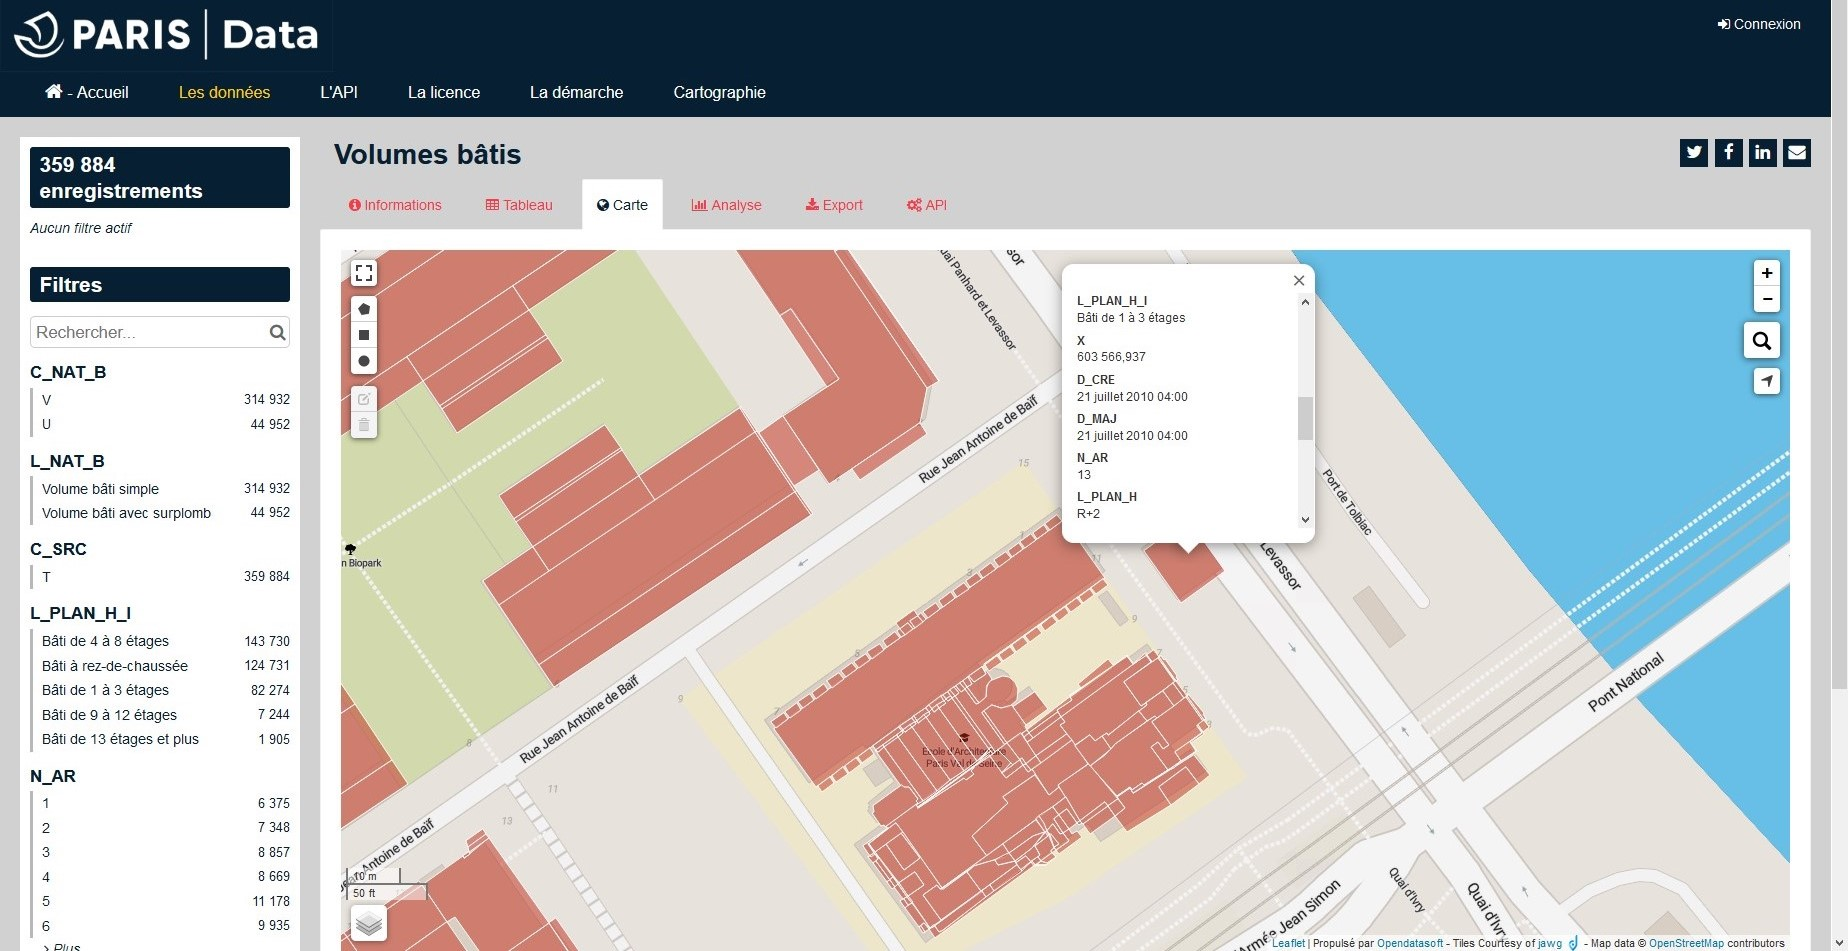
\includegraphics[width=0.9\linewidth]{__imgs/site_odp_carte} 

}

\caption[Prévisualisation cartographique du jeu de données des volumes bâtis.  -  https://opendata.paris.fr/]{Prévisualisation cartographique du jeu de données des volumes bâtis.}\label{fig:odp_carte}
\end{figure}
\end{tcolorbox}

\hfill\break

\hypertarget{variables-et-typologies-des-valeurs}{%
\subsubsection{Variables et typologies des
valeurs}\label{variables-et-typologies-des-valeurs}}

Le premier constat que l'on peut réaliser après avoir brièvement
interagi avec la carte est que le jeu de donnée associe un ensemble de
\textbf{variables} (dont la dénomination est commune à l'ensemble de ce
jeu) et leurs \textbf{valeurs} (possédant elles aussi une notation
spécifique) avec une \textbf{forme géométrique géolocalisée} sur un fond
de carte (en l'occurrence, ce sont des \textbf{polygones}, formes
géométriques les plus à même de représenter l'emprise en plan des
différents bâtiments).\\
~\\
Afin de permettre une lecture plus complémentaire, il paraît intéressant
de consulter le tableau fin d'avoir une vue plus ``centrée'' sur les
différentes variables et leurs valeurs.\\

\begin{tcolorbox}
\begin{figure}

{\centering 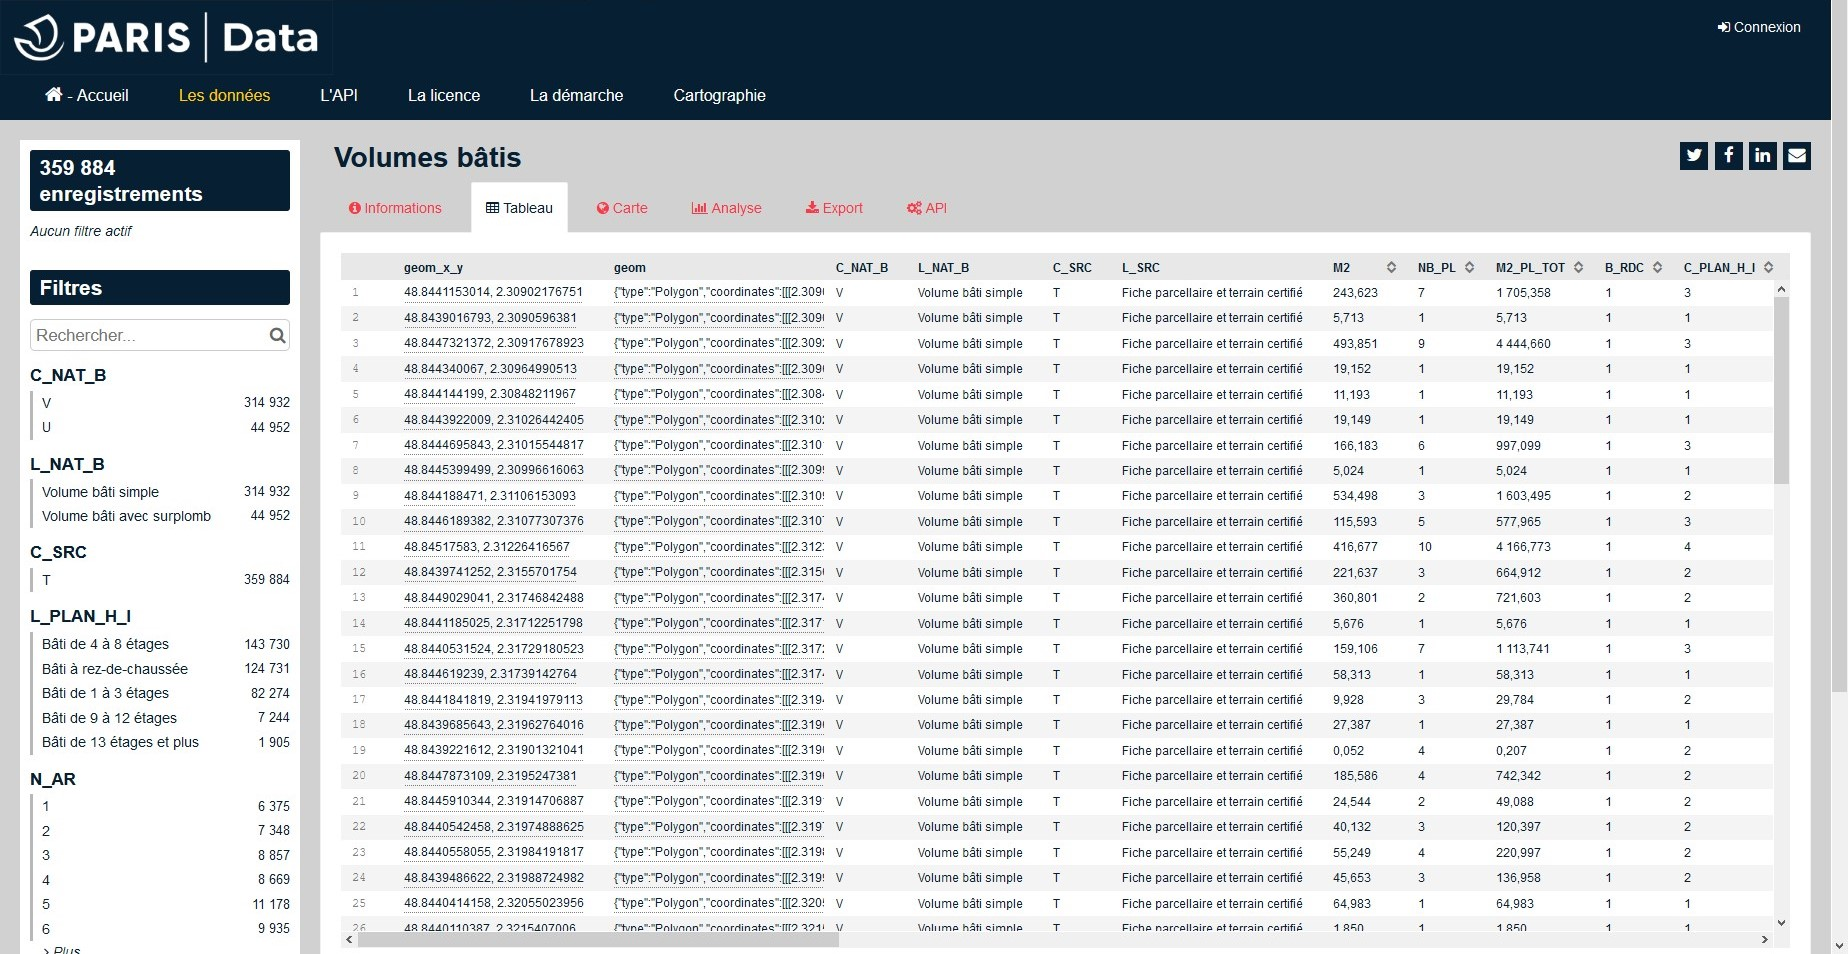
\includegraphics[width=0.9\linewidth]{__imgs/site_odp_tableau} 

}

\caption[Prévisualisation  du jeu de données des volumes bâtis sous forme de tableau.  -  https://opendata.paris.fr/]{Prévisualisation  du jeu de données des volumes bâtis sous forme de tableau.}\label{fig:odp_tbl}
\end{figure}
\end{tcolorbox}

\hfill\break
Chacune d'entre elles est ici représentée par une \textbf{colonne},
chaque ligne correspondant à un \textbf{volume bâti}. Tout d'abord, la
variable \emph{geom} est celle qui contient les informations
géométriques, nous renseignant sur le type de géométrie employée, ainsi
que les coordonnées des points qui la définissent. En l'occurence, la
typologie géométrique ``Polygon'' se base sur les types primitifs de
références des Systèmes d'Informations Géographiques (SIG), et ses
coordonnées sont définies en \textbf{latitude/longitude} (ce que
confirme la variable \emph{geom\_x\_y}).\\

\begin{tcolorbox}
\begin{figure}

{\centering 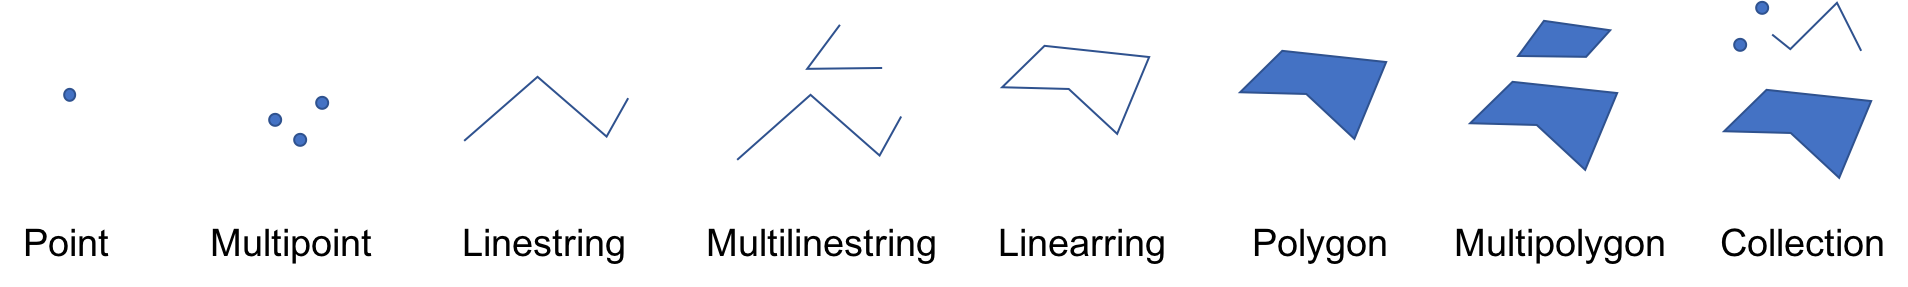
\includegraphics[width=0.9\linewidth]{__imgs/primitives_geometriques} 

}

\caption[Primitives géométriques des données géoréférencées  -  \url{https://github.com/ClementDelgrange/Cours_programmation_SIG/}]{Primitives géométriques des données géoréférencées}\label{fig:prim_geom}
\end{figure}
\end{tcolorbox}

\hfill\break
Nous pouvons également noter que certaines variables comme
\emph{L\_NAT\_B} ou \emph{L\_SRC} sont exprimées sous forme de texte,
qualifié alors de \textbf{``chaîne de caractères''} (``string'' ou
``str'' en anglais) d'un point de vue informatique. Elles semblent
également \textbf{catégoriques}, c'est à dire ne pouvant prendre qu'un
nombre défini de valeurs possibles. Bien que les noms de ces variables
ne soient pas explicites, leurs valeurs permettent d'avoir une première
idée de ce qu'elles renseignent.\\
~\\
A l'inverse, d'autres variables comme \emph{B\_RDC} ne possèdent ni un
nom explicite, ni une valeur permettant de suggérer sa signification,
étant catégorique mais notée sous forme d'\textbf{entiers}.\\
~\\
Enfin, d'autres variables comme \emph{M2} ou \emph{NB\_PL} sont notées
\textbf{numériquement}, pouvant à priori prendre une infinité de valeurs
, respectivement sous la forme de \textbf{réels} (ou nombres à virgule,
qualifiés de \emph{float} en anglais), et d'\textbf{entiers}
(\emph{int}). Bien que l'on puisse deviner que \emph{M2} semble
représenter la surface d'un volume bâti, cela reste une supposition.\\
~\\
Rappelons égalament que toutes ces observations sont faites sur un
échantillon visible d'un jeu de données massif. Certaines subtilités
présentes plus loin dans le tableau peuvent encore échapper à cette
lecture préliminaire.\\
~\\
Dès lors, chaque variable possédant sa \textbf{propre nomenclature}, et
étant plus ou moins explicite dans sa dénomination, une première
difficulté de lecture émerge. Heureusement, les jeux de données en Open
Data disposent généralement d'informations complémentaires capables de
renseigner l'utilisateur sur ces nomenclatures.\\

\hypertarget{les-muxe9tadonnuxe9es-cluxe9-de-compruxe9hension-des-donnuxe9es}{%
\subsubsection{Les métadonnées : clé de compréhension des
données}\label{les-muxe9tadonnuxe9es-cluxe9-de-compruxe9hension-des-donnuxe9es}}

Comme c'est le cas ici, la majorité des jeux de données accessibles en
Open Data disposent d'un document annexe de référence, dont le but est à
minima de fournir à l'utilisateur qui souhaite se saisir des données
contenues les explications nécessaires à la compréhension des variables
constituant le jeu de données en question. Ce sont \textbf{les
métadonnées}.\\
~\\
Elles peuvent également contenir des informations complémentaires
concernant le fournisseur, la manière dont les données ont été acquises
ou encore d'éventuelles limites de précision et recommandations
d'utilisation par exemple.\\

\begin{tcolorbox}
\begin{figure}

{\centering 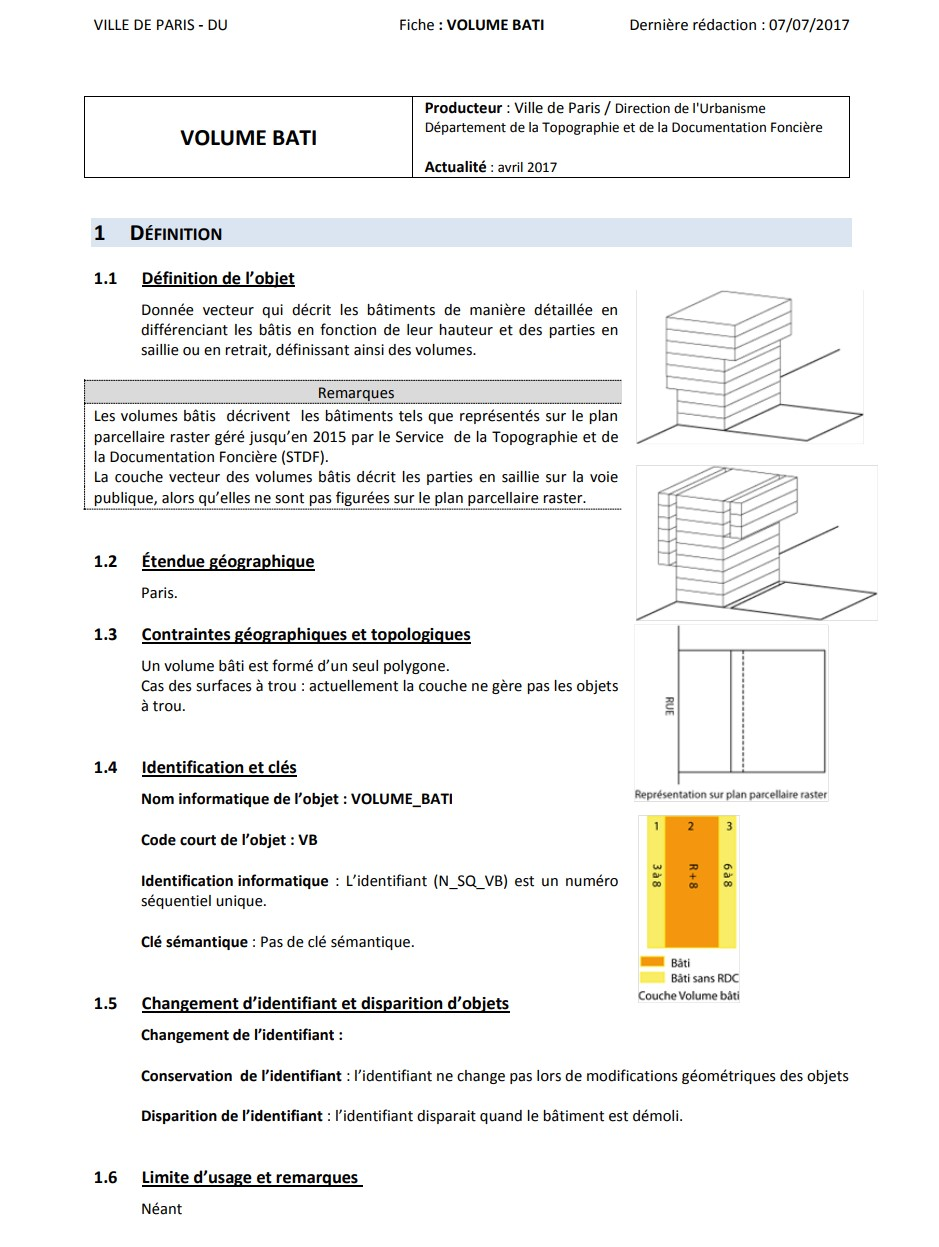
\includegraphics[width=0.9\linewidth]{__imgs/odp_meta1} 

}

\caption[Page descriptive issue des métadonnées  -  https://opendata.paris.fr/]{Page descriptive issue des métadonnées}\label{fig:odp_meta_1}
\end{figure}
\end{tcolorbox}

\hfill\break
En l'occurence, la première page nous renseigne de manière plus
exhaustive sur la manière dont ont été tracés les différents polygones,
à travers quelques schémas, ainsi qu'un paragraphe exprimant la source
de ces tracés. Premièrement, ce document explique sa logique de séparer
un bâtiment ``réel'' en plusieurs volumes fictifs, suivant s'ils sont en
porte à faux ou non, permettant d'apporter une certaine précision.\\
~\\
Dès lors, les deux informations primordiales associées à chaque polygone
sont sa \textbf{hauteur}, ainsi que ses différents \textbf{intervalles
de hauteur} s'il est en porte à faux. cette fiche indique également le
contexte géographique, ainsi que les limitations géométriques
(empêchants ici de représenter un polygone ``évidé'', obligeant à le
sectionner si l'on veut représenter de manière correcte un patio par
exemple).\\

\begin{tcolorbox}
\begin{figure}

{\centering 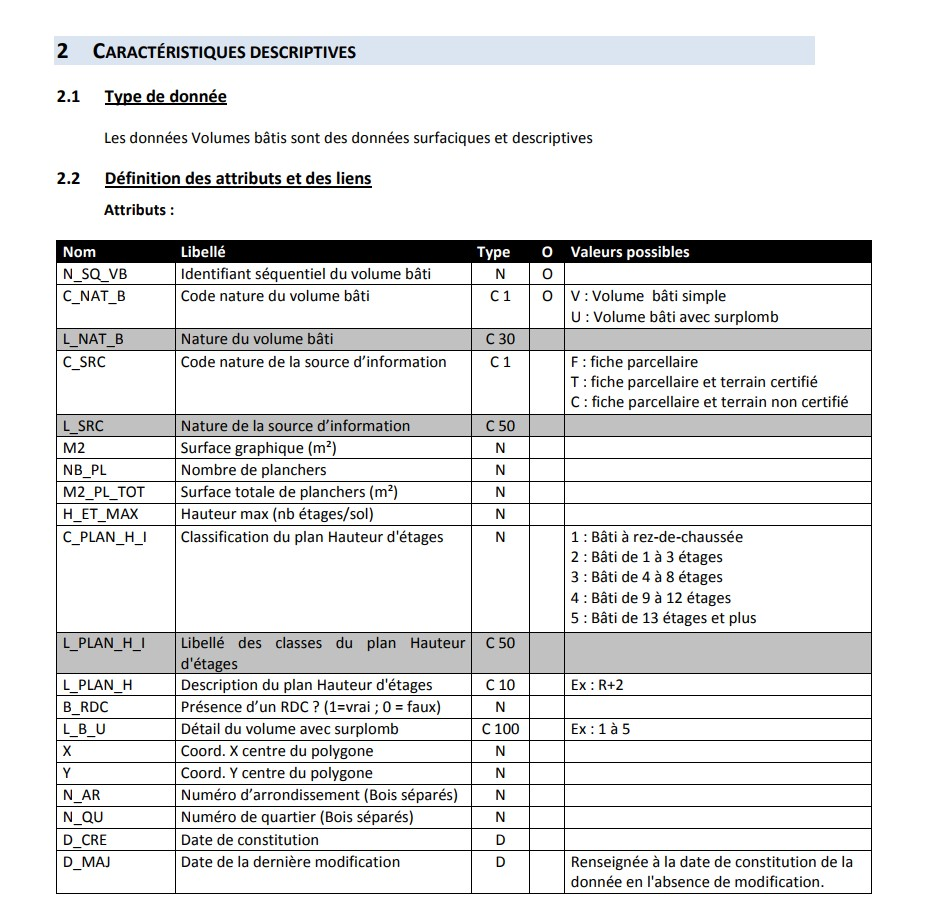
\includegraphics[width=0.9\linewidth]{__imgs/odp_meta2} 

}

\caption[Table descriptive des variables issue des métadonnées  -  https://opendata.paris.fr/]{Table descriptive des variables issue des métadonnées}\label{fig:odp_meta_2}
\end{figure}
\end{tcolorbox}

\hfill\break
Enfin, la seconde page contient les informations cruciales concernant
les données à exploiter.\\
En effet, le tableau-ci-dessus renseigne sur le \textbf{libellé} de
chaque variable (son contenu explicite), son \textbf{type} (ici,
\textbf{C\emph{n}} où \emph{n} est un entier signifie que les valeurs
sont sous forme textuelle de \emph{n} caractères de long, tandis que
\textbf{N} désigne simplement des valeurs numériques), ainsi que ses
valeurs possibles si ces dernières sont prédéfinies (servant à
distinguer les variables \textbf{catégoriques}).\\
Dès lors, il est possible de repérer les deux variables les plus
pertinentes si l'on souhaite extraire la hauteur des différents volumes.
En l'occurence, ce seront les variables \textbf{H\_ET\_MAX} ainsi que
\textbf{L\_B\_U} (pour les volumes en porte à faux), toutes deux
exprimées en nombre d'étages. La surface de plancher totale
\textbf{M2\_PL\_TOT} est également intéressante à extraire.\\
~\\
Ainsi, les métadonnées offrent les clés de compréhension nécessaires à
l'utilisateur afin de comprendre le contenu d'un jeu de données en
profondeur. Cette prise de connaissance permet désormais de manipuler
les données en elle-mêmes, au sein d'un script en Python.

\newpage

\hypertarget{le-langage-python-pour-sapproprier-aisuxe9ment-les-donnuxe9es-ouvertes}{%
\subsection{Le langage Python pour s'approprier aisément les données
ouvertes}\label{le-langage-python-pour-sapproprier-aisuxe9ment-les-donnuxe9es-ouvertes}}

Afin d'exploiter ce jeu de données constitué d'objets géolocalisées et
leurs données, le langage de programmation \textbf{Python} sera
exclusivement employé. Comme mentionné dans l'introduction, ce dernier
possède toutes les fonctionnalités nécessaires pour manipuler simplement
ce type de données.\\
~\\
La plateforme Open Data Paris permettant de définir un périmètre afin de
restreindre le jeu de données directement sur la carte, cette fonction
sera utilisée afin d'en télécharger un échantillon (en l'occurence
localisé autour de l'ENSAPVS).\\

\begin{tcolorbox}
\begin{figure}

{\centering 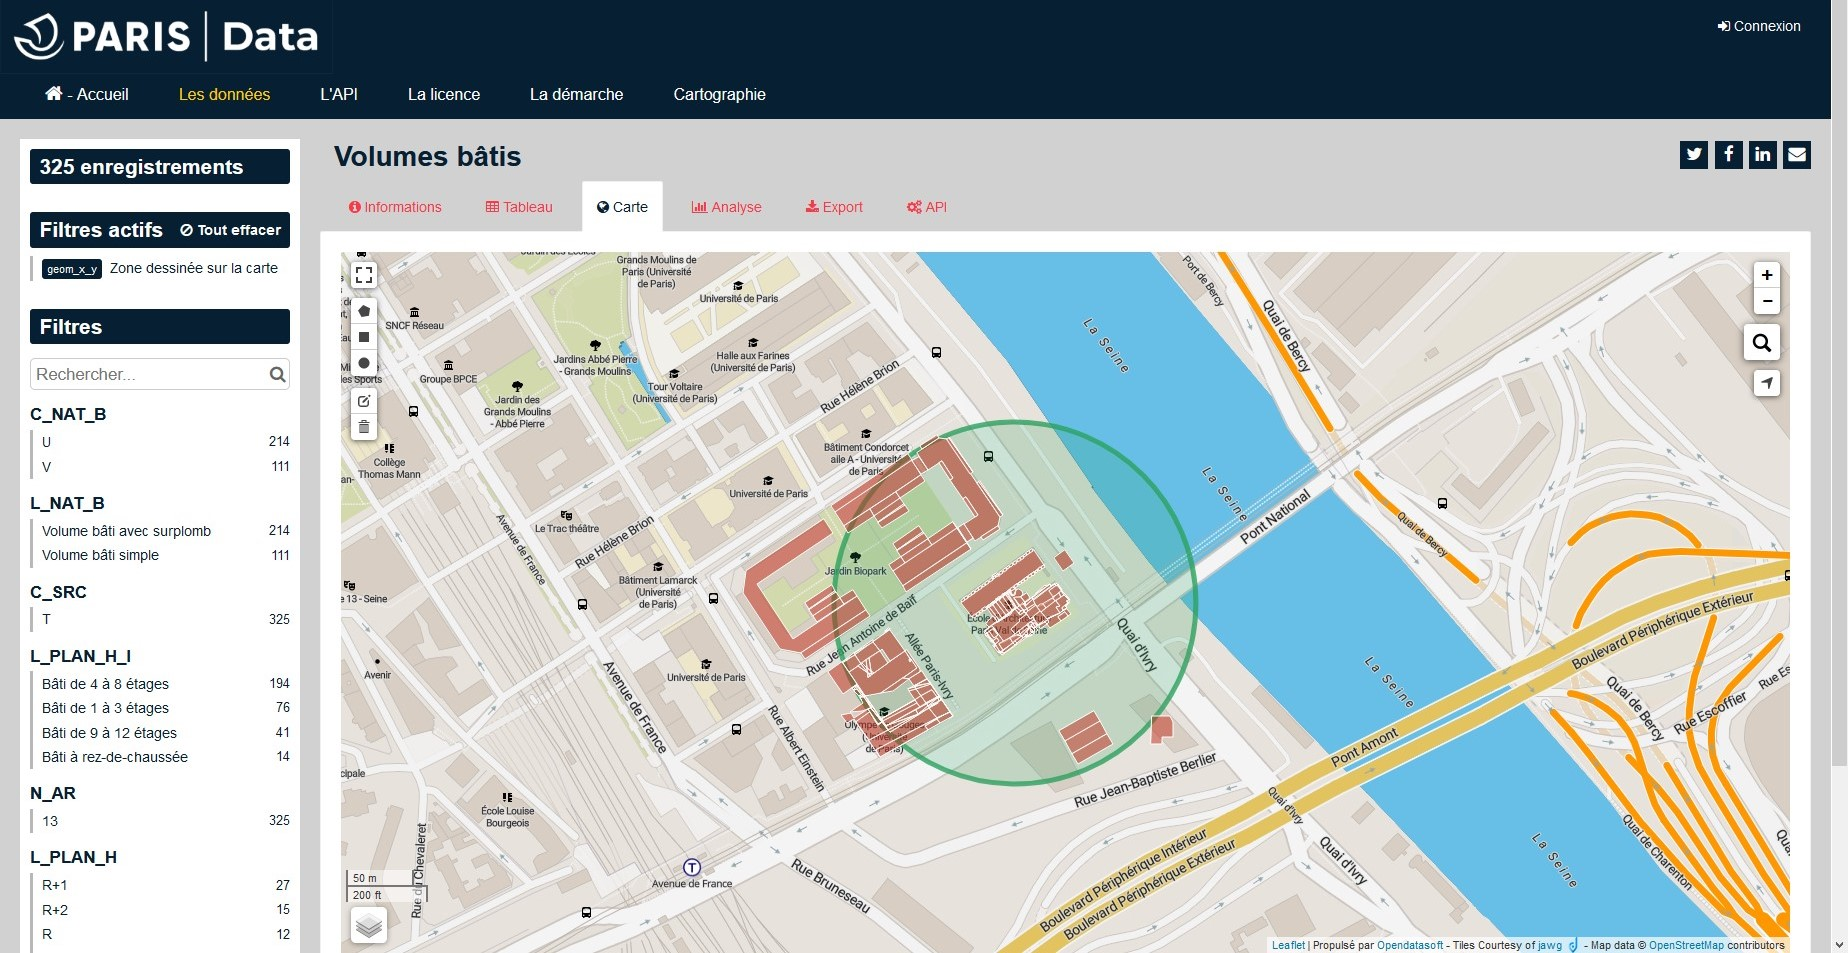
\includegraphics[width=0.9\linewidth]{__imgs/site_odp_carte_zone} 

}

\caption[Définition d'une zone d'extraction de données des volumes bâtis  -  https://opendata.paris.fr/]{Définition d'une zone d'extraction de données des volumes bâtis}\label{fig:odp_carte_zone}
\end{figure}
\end{tcolorbox}

\begin{tcolorbox}
\begin{figure}

{\centering 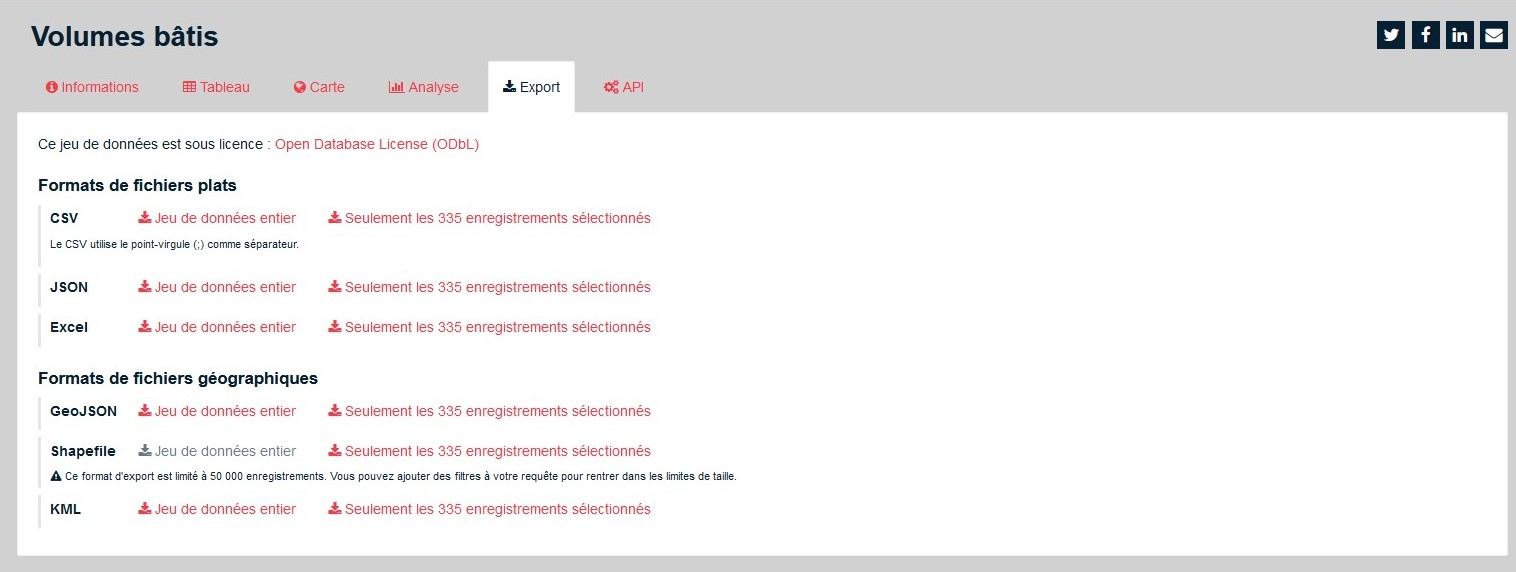
\includegraphics[width=0.9\linewidth]{__imgs/site_odp_formats} 

}

\caption[Un choix étendu de formats de fichiers  -  https://opendata.paris.fr/]{Un choix étendu de formats de fichiers}\label{fig:odp_formats}
\end{figure}
\end{tcolorbox}

A l'instar d'autres jeux de données, celui des ``volumes bâtis'' propose
\textbf{plusieurs formats} lors du téléchargement.\\
~\\
Dès lors, grâce à son large éventail de \textbf{bibliothèques}
(comparables à des ``extensions'') le langage Python se révèle ici
précieux car il est \textbf{capable de manipuler tous les formats de
fichiers proposés}. Or, le choix d'un format en particulier pourrait
alors être perçu comme un ``non-problème'', étant donné de telles
capacités. Ainsi, une \textbf{brève entrevue} sera apportée sur chacun
de ces formats grâce à Python, afin de déterminer lequel choisir.\\

\hypertarget{les-formats-tabulaires}{%
\subsubsection{Les formats tabulaires}\label{les-formats-tabulaires}}

\begin{tcolorbox}
\begin{figure}

{\centering 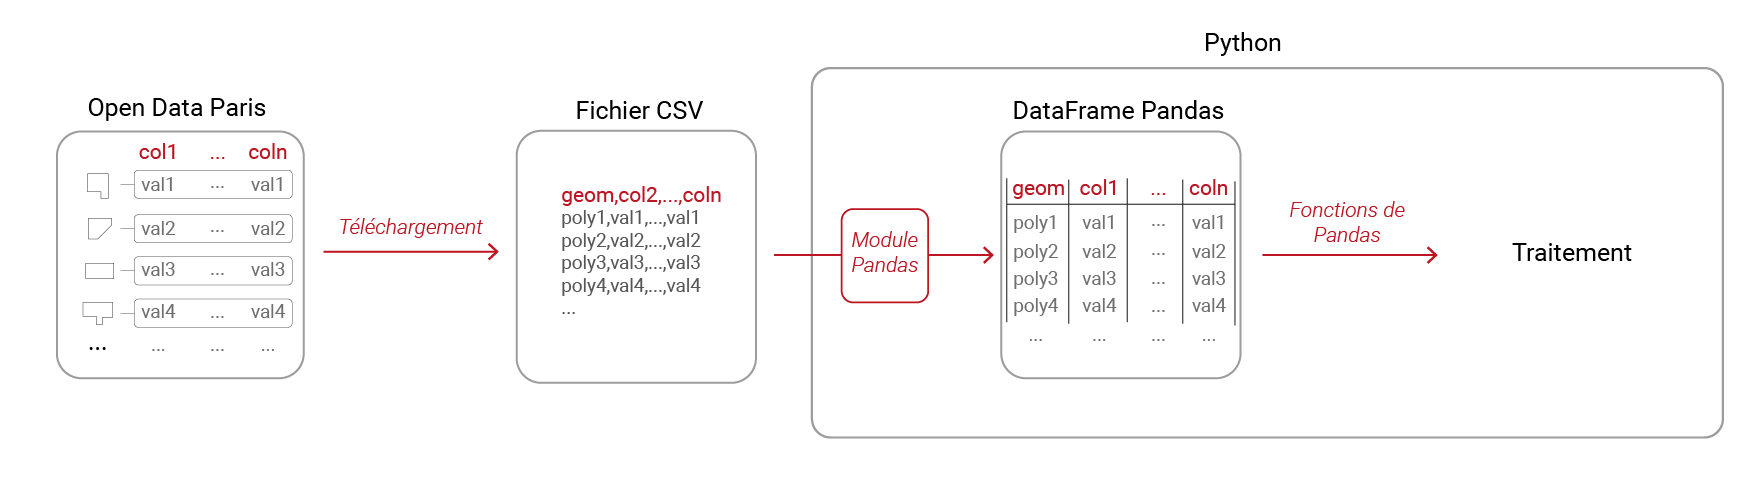
\includegraphics[width=0.9\linewidth]{__imgs/io_csv} 

}

\caption[Chargement du jeu de données sous un format tabulaire dans Python  -  réalisation personnelle]{Chargement du jeu de données sous un format tabulaire dans Python}\label{fig:io_csv}
\end{figure}
\end{tcolorbox}

\begin{tcolorbox}[title= Chargement du jeu de données sous un format tabulaire dans Python ,colback=boitecode]
\begin{lstlisting}[style=code]
# Import de la bibliothèque pandas
import pandas
# Lecture du fichier CSV
data = pandas.read_csv("DONNEES/volumesbatisparis.csv",sep=";")
# Affichage du premier élément de la colonne geom
geom = data["geom"][0]
print(type(geom))\end{lstlisting}

```
ttvar{#}ttvar{#} <class 'str'>
```

\end{tcolorbox}

Tout d'abord, les formats conventionnels de type tableur comme
\textbf{CSV} ou \textbf{Excel} représentent des choix inadaptés. En
effet, dû au fait que le tableur est limité à \textbf{un type de valeur
par colonne}, en l'occurence \textbf{soit du texte, soit des chiffres},
des variables telles que \textbf{GEOM}, d'une structure plus complexe
s'intègrent ici très mal. Cela peut être prouvé grâce à la bibliothèque
\textbf{Pandas}, spécialisée dans la manipulation de formats tableurs,
en recréant dans Python un objet nommé \emph{DataFrame}, composé de
lignes et de colonnes. En l'occurrence, la variable \textbf{GEOM} a
perdu sa structure, étant notée telle quelle sous forme de
\textbf{texte} (\emph{str}).

\hypertarget{les-formats-hiuxe9rarchisuxe9s}{%
\subsubsection{Les formats
hiérarchisés}\label{les-formats-hiuxe9rarchisuxe9s}}

\begin{tcolorbox}
\begin{figure}

{\centering 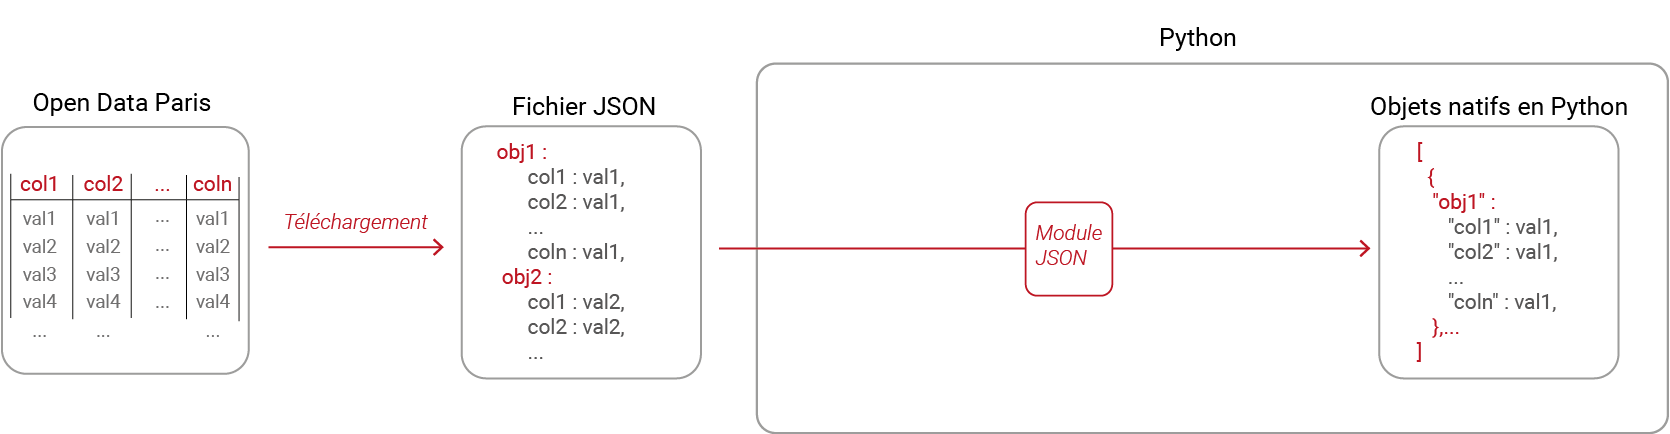
\includegraphics[width=0.9\linewidth]{__imgs/io_json} 

}

\caption[Chargement du jeu de données sous un format hiérarchisé dans Python  -  réalisation personnelle]{Chargement du jeu de données sous un format hiérarchisé dans Python}\label{fig:io_json}
\end{figure}
\end{tcolorbox}

\begin{tcolorbox}[title= Chargement du jeu de données sous un format hiérarchisé dans Python ,colback=boitecode]
\begin{lstlisting}[style=code]
# Import de la bibliothèque json
import json
# Lecture du fichier JSON
data = json.load(open("DONNEES/volumesbatisparis.json","r"))
# premier objet de la liste de volumes
print(data[0]["fields"]["geom"]["coordinates"])\end{lstlisting}

```
ttvar{#}ttvar{#} [[[2.38461935101913, 48.82753330722759], [2.384628217027156, 48.827532989502515], [2.3846363958367522, 48.82753065095026], [2.384645732926233, 48.82752608251942], [2.384652326040948, 48.82752179316423], [2.384656649382123, 48.827517191739766], [2.3846610231503442, 48.82751039520838], [2.38466170017297, 48.827501160346245], [2.3846595300456173, 48.827494714176034], [2.3846568869734233, 48.827489906925564], [2.384651922306437, 48.82748583150989], [2.384644105454289, 48.827480816864174], [2.384636766433263, 48.827477788690516], [2.384629481798523, 48.82747615392299], [2.384622830912725, 48.827475528812954], [2.3846147562394, 48.82747539282936], [2.384604096304909, 48.82747686151168], [2.384597659243542, 48.827478431967464], [2.384591275760087, 48.827481117919454], [2.384570429741702, 48.82747103121795], [2.384564292829435, 48.8274680613895], [2.384626028289865, 48.82741133372302], [2.384605980177239, 48.8274017376928], [2.384599619398239, 48.827398692965495], [2.384590133231389, 48.82740735276743], [2.384491575487986, 48.827497325948926], [2.384502471066941, 48.827502550714016], [2.384490396493715, 48.82751330891048], [2.384495045310945, 48.82751552280666], [2.38450719147041, 48.82750446998423], [2.3845183543743262, 48.82750978156396], [2.384548210954412, 48.827482266947136], [2.384554935749008, 48.82748540078928], [2.384576016445481, 48.82749522428569], [2.384573845038873, 48.827504696086415], [2.384575044805671, 48.82751060663542], [2.384577439054112, 48.82751606734975], [2.384581597086672, 48.82752085451733], [2.384586015415385, 48.827524477438544], [2.384592041213091, 48.827527975524475], [2.384603039948636, 48.827531501897994], [2.384612013974757, 48.82753299606446], [2.38461935101913, 48.82753330722759]]]
```

\end{tcolorbox}

Ensuite, le format \textbf{JSON} semble adapté à la structure de la
variable \textbf{GEOM}, permettant ici d'en extraire les
sous-informations. Cependant, il est nécessaire au préalable de
\textbf{lire le fichier en lui même} via un éditeur de texte, afin d'en
repérer la hiérarchie. Cette dernière se repose sur la \textbf{notation
objet}, une syntaxe commune à de nombreux langages de programmation
modernes comme le Python. Elle est constituée d'ensembles (listes) de
couples \textbf{attribut : valeur}, que l'on peut \textbf{hiérarchiser}
en les imbriquant.\\
~\\

\begin{tcolorbox}[title= Chargement du jeu de données sous un format hiérarchisé dans Python ,colback=boitecode]
\begin{lstlisting}[style=code]
expl = {\end{lstlisting}
\begin{lstlisting}[style=code]
        "datasetid": "volumesbatisparis",\end{lstlisting}
\begin{lstlisting}[style=code]
        "recordid": "9cb9b7143c595f9cd2b88e4d5bc588112fedc5a8",\end{lstlisting}
\begin{lstlisting}[style=code]
        "fields": {\end{lstlisting}
\begin{lstlisting}[style=code]
            "objectid": 536158,\end{lstlisting}
\begin{lstlisting}[style=code]
            "n_sq_pf": 750031416,\end{lstlisting}
\begin{lstlisting}[style=code]
            "d_maj": "2010-07-21T04:00:00+02:00",\end{lstlisting}
\begin{lstlisting}[style=code]
            "l_src": "Fiche parcellaire et terrain certifi\u00e9",\end{lstlisting}
\begin{lstlisting}[style=code]
            "l_b_u": "Ra1_et_encorbt_au_3",\end{lstlisting}
\begin{lstlisting}[style=code]
            "h_et_max": 3.0,\end{lstlisting}
\begin{lstlisting}[style=code]
            "b_rdc": 1.0,\end{lstlisting}
\begin{lstlisting}[style=code]
            "n_ar": 13,\end{lstlisting}
\begin{lstlisting}[style=code]
            "m2_pl_tot": 12.7752023,\end{lstlisting}
\begin{lstlisting}[style=code]
            "d_cre": "2010-07-21T04:00:00+02:00",\end{lstlisting}
\begin{lstlisting}[style=code]
            "m2": 4.2584008,\end{lstlisting}
\begin{lstlisting}[style=code]
            "l_plan_h_i": "B\u00e2ti de 1 \u00e0 3 \u00e9tages",\end{lstlisting}
\begin{lstlisting}[style=code]
            "n_sq_qu": 750000050,\end{lstlisting}
\begin{lstlisting}[style=code]
            "geom_x_y": [\end{lstlisting}
\begin{lstlisting}[style=code]
                48.8272714473,\end{lstlisting}
\begin{lstlisting}[style=code]
                2.38477660061\end{lstlisting}
\begin{lstlisting}[style=code]
            ],\end{lstlisting}
\begin{lstlisting}[style=code]
            "l_nat_b": "Volume b\u00e2ti avec surplomb",\end{lstlisting}
\begin{lstlisting}[style=code]
            "n_qu": 50.0,\end{lstlisting}
\begin{lstlisting}[style=code]
            "c_plan_h_i": 2.0,\end{lstlisting}
\begin{lstlisting}[style=code]
            "shape_area": 0.0,\end{lstlisting}
\begin{lstlisting}[style=code]
            "c_src": "T",\end{lstlisting}
\begin{lstlisting}[style=code]
            "nb_pl": 3.0,\end{lstlisting}
\begin{lstlisting}[style=code]
            "n_sq_vb": 750170119,\end{lstlisting}
\begin{lstlisting}[style=code]
            "shape_len": 0.0,\end{lstlisting}
\begin{lstlisting}[style=code]
            "c_nat_b": "U",\end{lstlisting}
\begin{lstlisting}[style=code]
            "geom": {\end{lstlisting}
\begin{lstlisting}[style=code]
                "type": "Polygon",\end{lstlisting}
\begin{lstlisting}[style=code]
                "coordinates": [\end{lstlisting}
\begin{lstlisting}[style=code]
                    [\end{lstlisting}
\begin{lstlisting}[style=code]
                        [\end{lstlisting}
\begin{lstlisting}[style=code]
                            2.384770481308271,\end{lstlisting}
\begin{lstlisting}[style=code]
                            48.827286816032526\end{lstlisting}
\begin{lstlisting}[style=code]
                        ],\end{lstlisting}
\begin{lstlisting}[style=code]
                        [\end{lstlisting}
\begin{lstlisting}[style=code]
                            2.384796971933453,\end{lstlisting}
\begin{lstlisting}[style=code]
                            48.82726286263405\end{lstlisting}
\begin{lstlisting}[style=code]
                        ],\end{lstlisting}
\begin{lstlisting}[style=code]
                        [\end{lstlisting}
\begin{lstlisting}[style=code]
                            2.384782602464847,\end{lstlisting}
\begin{lstlisting}[style=code]
                            48.8272560560162\end{lstlisting}
\begin{lstlisting}[style=code]
                        ],\end{lstlisting}
\begin{lstlisting}[style=code]
                        [\end{lstlisting}
\begin{lstlisting}[style=code]
                            2.384756236578184,\end{lstlisting}
\begin{lstlisting}[style=code]
                            48.82728017373901\end{lstlisting}
\begin{lstlisting}[style=code]
                        ],\end{lstlisting}
\begin{lstlisting}[style=code]
                        [\end{lstlisting}
\begin{lstlisting}[style=code]
                            2.384770481308271,\end{lstlisting}
\begin{lstlisting}[style=code]
                            48.827286816032526\end{lstlisting}
\begin{lstlisting}[style=code]
                        ]\end{lstlisting}
\begin{lstlisting}[style=code]
                    ]\end{lstlisting}
\begin{lstlisting}[style=code]
                ]\end{lstlisting}
\begin{lstlisting}[style=code]
            },\end{lstlisting}
\begin{lstlisting}[style=code]
            "n_sq_ar": 750000013,\end{lstlisting}
\begin{lstlisting}[style=code]
            "y": 125199.7506478,\end{lstlisting}
\begin{lstlisting}[style=code]
            "x": 603542.699385\end{lstlisting}
\begin{lstlisting}[style=code]
      }\end{lstlisting}
\begin{lstlisting}[style=code]
  }\end{lstlisting}
\end{tcolorbox}

\hfill\break
\hfill\break
Dès lors, une fois cette notation assimilée, ce format permet une
lecture relativement \textbf{aisée} pour l'utilisateur, tout en restant
\textbf{simple} à lire par la machine. Le code d'extraction découle donc
naturellement de la lecture humaine.

\hypertarget{les-formats-guxe9ographiques}{%
\subsubsection{Les formats
géographiques}\label{les-formats-guxe9ographiques}}

Enfin, puisque le jeu de données en question est constitué
\textbf{d'objets géoréférencés}, les formats \textbf{GeoJSON},
\textbf{Shapefile} et \textbf{KML} semblent être les formats les plus
adaptés. Or, chacun de ces formats possède \textbf{sa propre notation
normée pour les données géographiques}, ce qui nécessite habituellement
l'utilisation d'outils spécifiques comme \textbf{QGIS} afin de les
lire.\\
~\\
~\\
Cependant, le langage Python possède une bibliothèque nommée
\textbf{GeoPandas} spécialisée dans la \textbf{manipulation de données
géoréférencées}. De manière similaire à la bibliothèque \textbf{Pandas}
montrée plus haut, elle permet de traduire une collection
d'\textbf{objets géoréférencés} en un objet \emph{DataFrame} similaire à
un tableur, cette fois-ci sans limitations au niveau des types de
données. En outre, cette représentation prodigue un grand nombre de
\textbf{fonctions} appliquables aux lignes et aux colonnes permettant
par la suite d'opérer des transformations de manière aisée.

\begin{tcolorbox}
\begin{figure}

{\centering 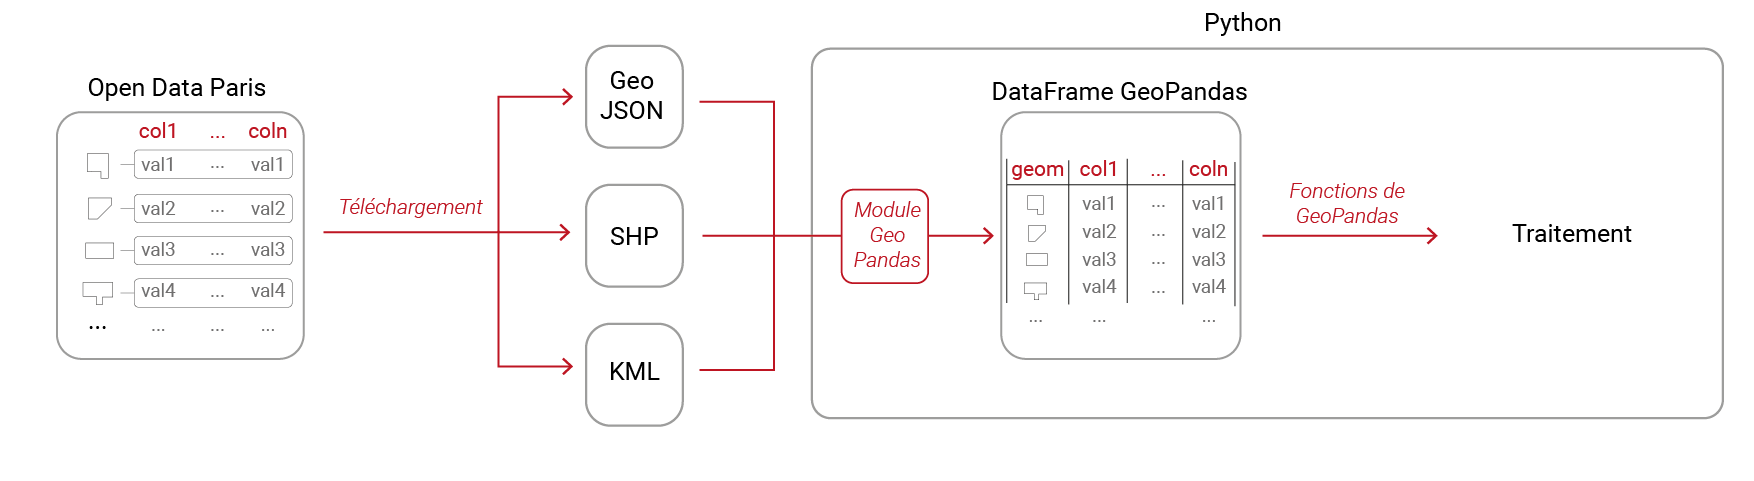
\includegraphics[width=0.9\linewidth]{__imgs/io_gpd} 

}

\caption[Chargement du jeu de données sous un format géographique dans Python  -  réalisation personnelle]{Chargement du jeu de données sous un format géographique dans Python}\label{fig:io_gpd}
\end{figure}
\end{tcolorbox}

\begin{tcolorbox}[title= Chargement du jeu de données sous un format géographique dans Python ,colback=boitecode]
\begin{lstlisting}[style=code]
# Import de géopandas sous l'acronyme gpd
import geopandas as gpd
# Spécification nécessaire à la lecture du KML
gpd.io.file.fiona.drvsupport.supported_drivers['KML'] = 'rw'
# Lecture du fichier KML et du premier objet de la colonne "geom"
data = gpd.read_file("DONNEES/volumesbatisparis.kml", driver='KML')
print(data.head(1))
# Lecture du fichier SHP et du premier objet de la colonne "geom"\end{lstlisting}

```
ttvar{#}ttvar{#}   Name Description                                           geometry
ttvar{#}ttvar{#} 0    V              POLYGON ((2.38462 48.82753, 2.38461 48.82753, ...
```

\begin{lstlisting}[style=code]
data = gpd.read_file("DONNEES/volumesbatisparis.shp")
print(data.head(1))
# Lecture du fichier GeoJSON et du premier objet de la colonne "geom"\end{lstlisting}

```
ttvar{#}ttvar{#}   c_nat_b              l_nat_b c_src                                   l_src         m2  nb_pl   m2_pl_tot  b_rdc  c_plan_h_i              y  ...  n_qu  objectid      n_sq_vb      n_sq_ar      n_sq_pf      n_sq_qu du_stdf_vol  shape_area  shape_len                                           geometry
ttvar{#}ttvar{#} 0       V  Volume bâti simple     T  Fiche parcellaire et terrain certifié  70.303737    4.0  281.214948    1.0         2.0  125224.417845  ...  50.0  536092.0  750169268.0  750000013.0  750031416.0  750000050.0        None         0.0        0.0  POLYGON ((2.38462 48.82753, 2.38463 48.82753, ...
ttvar{#}ttvar{#} 
ttvar{#}ttvar{#} [1 rows x 28 columns]
```

\begin{lstlisting}[style=code]
data = gpd.read_file("DONNEES/volumesbatisparis.geojson")
print(data.head(1))\end{lstlisting}

```
ttvar{#}ttvar{#}    objectid      n_sq_pf                d_maj                                  l_src l_plan_h  h_et_max  b_rdc  n_ar   m2_pl_tot                d_cre  ...  c_src nb_pl    n_sq_vb shape_len  c_nat_b    n_sq_ar              y              x  l_b_u                                           geometry
ttvar{#}ttvar{#} 0    536092  750031416.0  2010-07-21T04:00:00  Fiche parcellaire et terrain certifié      R+3       3.0    1.0    13  281.214948  2010-07-21T04:00:00  ...      T   4.0  750169268       0.0        V  750000013  125224.417845  603527.957994   None  POLYGON ((2.38462 48.82753, 2.38463 48.82753, ...
ttvar{#}ttvar{#} 
ttvar{#}ttvar{#} [1 rows x 27 columns]
```

\end{tcolorbox}

De plus, \textbf{les objets géoréférencés} sont automatiquement
convertis en formes géométriques, permettant d'y appliquer des
manipulations géométriques spécifiques.

\begin{tcolorbox}[title= Chargement du jeu de données sous un format géographique dans Python ,colback=boitecode]
\begin{lstlisting}[style=code]
# Calcul du centroide pour le premier objet en une seule ligne
print(data["geometry"][0].centroid)\end{lstlisting}

```
ttvar{#}ttvar{#} POINT (2.384586335419862 48.82747966979255)
```

\end{tcolorbox}

Pour toutes ses qualités, cette approche avec \textbf{GeoPandas} sera
privilégiée à travers les chapitres suivants. Enfin, quant au format de
fichier en lui-même, le \textbf{GeoJSON} sera ici arbitrairement
choisi.\\
~\\
Ainsi, grâce à une \textbf{immense compatibilité} avec la majorité des
types de formats courants en Open Data (prodiguée par ses nombreuses
bibliothèques), le langage Python constitue d'ores-et-déjà un formidable
outil d'extraction, permettant de \textbf{s'approprier facilement} des
jeux de données à la \textbf{structure complexe}. Cependant, son
véritable intérêt réside dans son statut de langage de programmation,
étant alors capable de traitements automatiques avancés.

\newpage

\hypertarget{aperuxe7u-de-la-souplesse-des-fonctions-de-manipulation-de-donnuxe9es}{%
\subsection{Aperçu de la souplesse des fonctions de manipulation de
données}\label{aperuxe7u-de-la-souplesse-des-fonctions-de-manipulation-de-donnuxe9es}}

Après la phase d'extraction précédente, il est nécessaire que les
données etraites en l'état soient exploitables pour la suite.

Premièrement, le jeu de données sera réduit aux variables identifiées
lors de la lecture des métadonnées (à savoir
\textbf{GEOM},\textbf{M2\_PL\_TOT},\textbf{H\_ET\_MAX} ainsi que
\textbf{L\_B\_U}), et seront renommées afin d'être plus facilement
lisible par la suite.

\begin{tcolorbox}[title= Chargement du jeu de données sous un format géographique dans Python ,colback=boitecode]
\begin{lstlisting}[style=code]
data = data[["geometry","m2_pl_tot","h_et_max","l_b_u"]]
data = data.rename(columns={
    "m2_pl_tot" : "surface",
    "h_et_max" : "hauteur",
    "l_b_u" : "hauteur_paf"
    })
print(data)\end{lstlisting}

```
ttvar{#}ttvar{#}                                               geometry      surface  hauteur          hauteur_paf
ttvar{#}ttvar{#} 0    POLYGON ((2.38462 48.82753, 2.38463 48.82753, ...   281.214948      3.0                 None
ttvar{#}ttvar{#} 1    POLYGON ((2.38475 48.82722, 2.38476 48.82721, ...     9.842935      8.0                  5a8
ttvar{#}ttvar{#} 2    POLYGON ((2.38493 48.82732, 2.38495 48.82730, ...    52.982843      9.0           Ra1_et_3a9
ttvar{#}ttvar{#} 3    POLYGON ((2.38354 48.82665, 2.38323 48.82652, ...   229.771164      8.0                  2a8
ttvar{#}ttvar{#} 4    POLYGON ((2.38304 48.82670, 2.38315 48.82659, ...   310.513295      9.0                  3a9
ttvar{#}ttvar{#} ..                                                 ...          ...      ...                  ...
ttvar{#}ttvar{#} 330  POLYGON ((2.38469 48.82720, 2.38469 48.82720, ...     1.632114      4.0                  2a4
ttvar{#}ttvar{#} 331  POLYGON ((2.38451 48.82752, 2.38452 48.82751, ...     3.082522      3.0    R_et_encorbt_au_3
ttvar{#}ttvar{#} 332  POLYGON ((2.38453 48.82753, 2.38454 48.82752, ...     5.338095      5.0  Ra1_et_encorbt_au_5
....

```

\end{tcolorbox}

Dès lors, il serait souhaitable d'exprimer les hauteurs en
\textbf{mètres} plutôt qu'en nombre de niveaux.

\begin{tcolorbox}[title= Chargement du jeu de données sous un format géographique dans Python ,colback=boitecode]
\begin{lstlisting}[style=code]
h_etage = 3
print(data["hauteur"][0] * h_etage)\end{lstlisting}

```
ttvar{#}ttvar{#} 9.0
```

\end{tcolorbox}

Cette opération est triviale pour l'attribut \textbf{hauteur}, étant
exprimé numériquement. Il suffit alors de définir une \textbf{hauteur
d'étage type} et d'effectuer une multiplication.\\
Cependant, l'attribut \textbf{hauteur\_paf} étant exprimé sous la forme
de \textbf{texte} (chaînes de caractères) décrivant les plages de
hauteur, il est nécessaire de convertir cette notation numériquement
afin d'effectuer cette multiplication.

\hypertarget{approche-compruxe9hensive-des-diffuxe9rentes-notations-gruxe2ce-uxe0-python}{%
\subsubsection{Approche compréhensive des différentes notations grâce à
Python}\label{approche-compruxe9hensive-des-diffuxe9rentes-notations-gruxe2ce-uxe0-python}}

Heureusement, Python est capable de reconnaître des morceaux de texte au
sein de chaînes de caractères, permettant ainsi de les remplacer par
leur équivalent numérique.

\begin{tcolorbox}[title= Chargement du jeu de données sous un format géographique dans Python ,colback=boitecode]
\begin{lstlisting}[style=code]
if "da" in "data":
  print(1)
else:
  print(0)\end{lstlisting}

```
ttvar{#}ttvar{#} 1
```

\end{tcolorbox}

Dès lors, afin de comprendre les différentes manières d'exprimer les
hauteurs en porte à faux, il est possible de les énumérer par la
\textbf{longueur de leur texte} de chacune des notations.\\
~\\
Pour ce faire, un \textbf{dictionnaire} vide sera préalablement créé.
C'est le type de donnée utilisé en Python afin de représenter la
notation objet, en associant un \textbf{attribut} (sous forme de texte
ou d'entiers) avec une \textbf{valeur} (pouvant être de type varié).

\begin{tcolorbox}[title= Chargement du jeu de données sous un format géographique dans Python ,colback=boitecode]
\begin{lstlisting}[style=code]
# Dictionnaire à deux objets
d = {"A" : 10, "B" : 15}
# Récupération de la valeur associée à "A"
print(d["A"])
# Changement de la valeur associée à "B"\end{lstlisting}

```
ttvar{#}ttvar{#} 10
```

\begin{lstlisting}[style=code]
d["B"] = 30
print(d["B"])\end{lstlisting}

```
ttvar{#}ttvar{#} 30
```

\end{tcolorbox}

Une \textbf{boucle} avec \textbf{for} servira ensuite à itérer à travers
les différentes notations de la variable \textbf{l\_b\_u}.

\begin{tcolorbox}[title= Chargement du jeu de données sous un format géographique dans Python ,colback=boitecode]
\begin{lstlisting}[style=code]
# Liste de valeurs
l = [0,1,2,"trois"]

for item in l:
  print(item)\end{lstlisting}

```
ttvar{#}ttvar{#} 0
ttvar{#}ttvar{#} 1
ttvar{#}ttvar{#} 2
ttvar{#}ttvar{#} trois
```

\end{tcolorbox}

Comme le montre le code ci-dessous, pour chaque objet (\textbf{for}
\emph{objet}) contenu dans la liste l (\emph{in} \emph{l}), la boucle
affecte un nom de variable défini (ici, \textbf{item}), permettant
d'opérér sur chaque objet individuellement.\\
~\\

Ainsi, en itérant à travers chaque notation contenue dans la colonne
\textbf{hauteur\_paf}, un \textbf{exemple de notation} sera affecté au
dictionnaire vide créé précédemment en prennant comme attribut sa
\textbf{longueur}. En réalité, pour chaque longueur, c'est la dernière
notation qui sera conservée, chacune d'elle écrasant la précédente.
Enfin, la fonction \emph{dropna()} est employée ici pour supprimer les
valeurs nulles pour les volumes non-concernés.

\begin{tcolorbox}[title= Chargement du jeu de données sous un format géographique dans Python ,colback=boitecode]
\begin{lstlisting}[style=code]
# Création d'un dictionnaire vide
notations = {}
# Itération à travers la colonne "l_b_u"
for txt in data["hauteur_paf"].dropna():
  notations[len(txt)] = txt
print(notations)\end{lstlisting}

```
ttvar{#}ttvar{#} {3: '2a4', 10: '2a4_et_7a8', 12: 'encorbt_au_5', 19: 'Ra1_et_encorbt_au_5', 8: 'R_et_3a9', 9: 'Auvent_n1', 4: '4a11', 17: 'R_et_encorbt_au_3', 15: 'Ra1_et_3_et_5a8'}
```

\end{tcolorbox}

Dès lors, certains éléments constituants peuvent être notés :

\begin{itemize}
\tightlist
\item
  Une plage de hauteur est principalement renseignée par ses
  \textbf{deux niveaux de hauteur} séparées par un \emph{a}
\item
  \emph{\emph{et}} est utilisé pour renseigner \textbf{plusieurs plages
  de hauteur}.
\item
  \emph{``encorbt\_au\_N''} désigne une plage de hauteur du niveau
  \textbf{N} au niveau maximal (exprimé par la variable ``hauteur'').
  S'ils désignent le même niveau, la plage sera du niveau
  \textbf{N\textsuperscript{-1}} au niveau maximal.
\item
  \emph{auvent} désigne une plage du niveau \textbf{N} à
  \textbf{N\textsuperscript{+1}}.
\item
  Enfin, la présence de \emph{R} exprimé seul suggère que \textbf{R}
  désigne une plage d'une \textbf{seule hauteur d'étage partant du sol},
  tandis que \textbf{Ra1} désigne \textbf{deux hauteurs d'étages partant
  du sol}.
\end{itemize}

\begin{tcolorbox}
\begin{figure}

{\centering 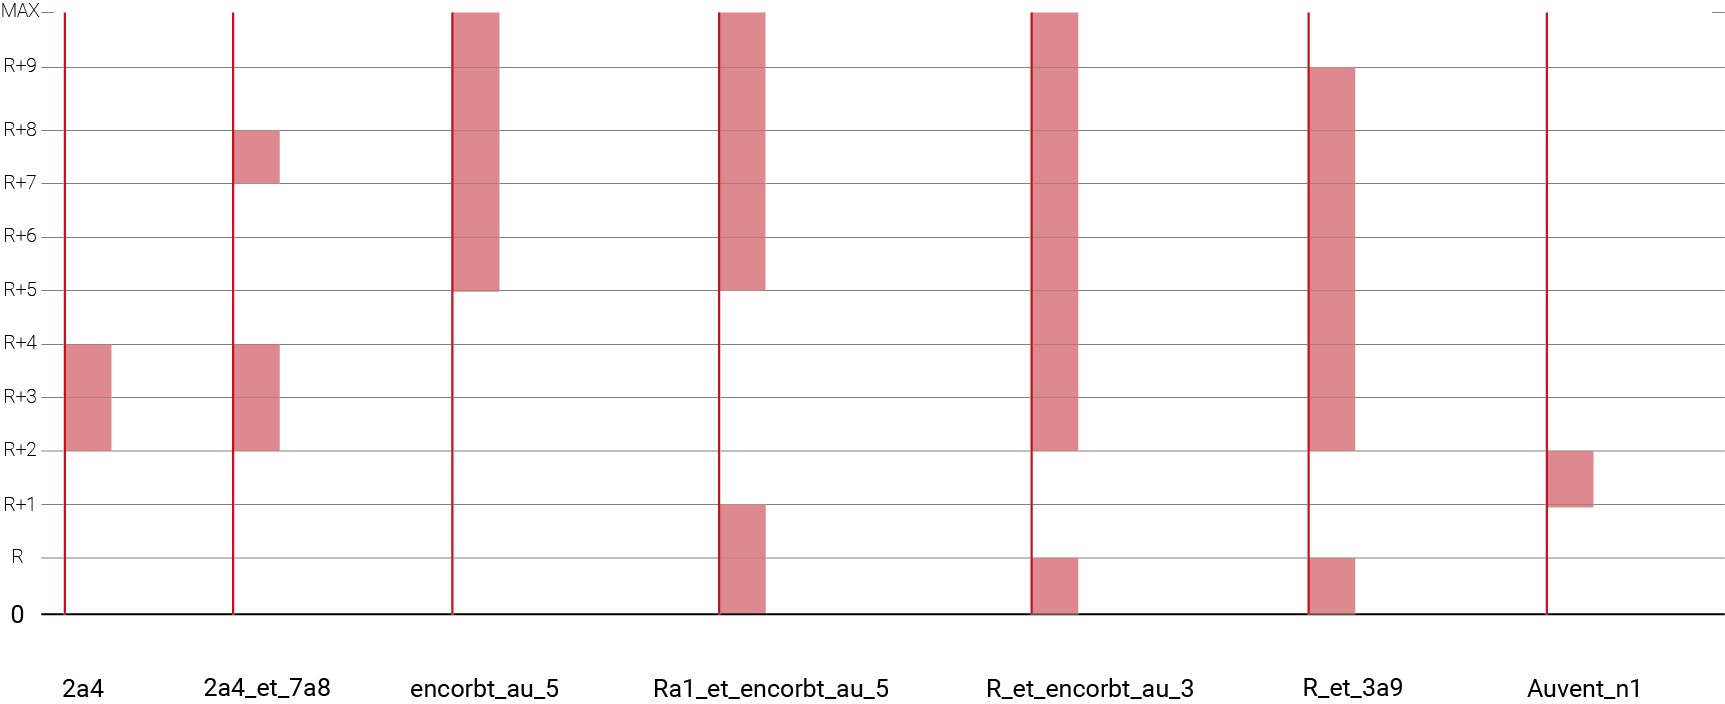
\includegraphics[width=0.9\linewidth]{__imgs/hpaf} 

}

\caption[Aperçu des différentes notations caractérisant les porte à faux  -  Réalisation personnelle]{Aperçu des différentes notations caractérisant les porte à faux}\label{fig:hpaf}
\end{figure}
\end{tcolorbox}

Cette dernière observation est cruciale : si l'on fixe \textbf{R = 0},
alors la plage \textbf{Ra1} devient \textbf{0a1}. Or, si l'on multiplie
ces deux bornes par la hauteur d'étage type de 3 mètres, le volume aura
une plage de hauteur de \textbf{0 à 3m}, tandis qu'il faudrait obtenir
\textbf{0 à 6m}. Dès lors, il faut \textbf{ajouter 1 à tout nombre de
niveau sauf R} avant multiplication par la hauteur d'étage type.

\hypertarget{de-la-chauxeene-de-caractuxe8re-uxe0-la-valeur-numuxe9rique}{%
\subsubsection{De la chaîne de caractère à la valeur
numérique}\label{de-la-chauxeene-de-caractuxe8re-uxe0-la-valeur-numuxe9rique}}

A la lumière de toutes ces subtilités, il est désormais possible de
créer une fonction capable de \textbf{transformer des chaînes de
caractères} en \textbf{valeurs numériques}. Le code ci-dessous illustre
la transformation d'une notation
\textbf{N\textsuperscript{1}aN\textsuperscript{2}}. Après s'être assuré
que la notation contient bien un \emph{a}, le code sépare les deux
bornes à cet endroit, puis les convertit en \textbf{entiers}. Enfin,
chaque borne est incrémentée de \textbf{1} avant multiplication par la
hauteur d'étage type, sauf \emph{R} qui prend la valeur 0.

\begin{tcolorbox}[title= Aperçu des différentes notations caractérisant les porte à faux ,colback=boitecode]
\begin{lstlisting}[style=code]
# Rappel : h_etage = 3 mètres
h_paf =  "Ra8"
if "a" in h_paf:
  # Séparation des deux chiffres au niveau du "a"
  hauteur = h_paf.split("a")
  # Conversion de chaque chiffre en entier, puis multiplication par la hauteur d'étage type
  # Si "R" est présent, il prend la valeur 0
  hauteur = [(int(h)+1)*h_etage if h != "R" else 0 for h in hauteur]

print(hauteur)\end{lstlisting}

```
ttvar{#}ttvar{#} [0, 27]
```

\end{tcolorbox}

Suivant ce principe, la \textbf{fonction} suivante opèrera ce type de
transformation suivant les différents notations relevées précédemment
sur l'ensemble des volumes. Une \textbf{fonction} est un bloc de code
que l'on définit \textbf{une seule fois} dans un script avec un
\textbf{nom} et éventuellement des \textbf{arguments} (paramètres), et
que l'on peut exécuter autant de fois que l'on souhaite par la suite en
l'appelant par son nom. Ici, cette fonction sera appelée
\textbf{texte\_to\_num}, et prendra pour argument chaque volume, afin de
convertir la notation caractérisant son porte à faux en expression
numérique. Elle appliquera également la transformation de la variable
\textbf{hauteur} (à savoir un incrément de 1 suivi d'une multiplication
par la hauteur d'étage type).

\begin{tcolorbox}[title= Aperçu des différentes notations caractérisant les porte à faux ,colback=boitecode]
\begin{lstlisting}[style=code]
# Rappel : h_etage = 3 mètres
def texte_to_num(volume):
     # Si le volume n'est pas en porte à faux
    if volume["hauteur_paf"] == None:
        # Affecter une valeur nulle
        volume["hauteur_paf"] = None
    else:
        # Liste vide pour contenir les notations numériques
        output = []
        # Séparation des sous-notations au niveau du "_et_"
        # Si absent, la notation sera conservée telle quelle
        intervalles = volume["hauteur_paf"].split("_et_")
        # Itération à travers les sous-notations
        for interv in intervalles:
            # filtrage par syntaxe
            if "encorbt_au_" in interv:
                n = int(interv.strip("encorbt_au_"))
                if n == volume["hauteur"]:
                    output.append([n*h_etage,(n+1)*h_etage])
                else:
                    output.append([(n+1)*h_etage,(volume["hauteur"]+1)*h_etage])
            elif "auvent_n" in interv:
                n = int(interv.strip("auvent_n"))
                output.append([n*h_etage,(n+1)*h_etage])
            elif "a" in interv:
                if "R" in interv:
                    output.append([0,(int(interv.strip("Ra"))+1)*h_etage])
                else:
                    output.append([(int(h)+1)*h_etage for h in interv.split("a")])
            elif interv == "R":
                output.append([0,h_etage])
            # Remplacement par la notation numérique
            volume["hauteur_paf"] = output

    volume["hauteur"] = (volume["hauteur"] + 1)*h_etage
    return volume\end{lstlisting}
\end{tcolorbox}

Enfin, cette fonction peut-être appliquée automatiquement à l'ensemble
du jeu.

\begin{tcolorbox}[title= Aperçu des différentes notations caractérisant les porte à faux ,colback=boitecode]
\begin{lstlisting}[style=code]
# Application à chaque volume avec .apply()
data = data.apply(lambda volume : texte_to_num(volume),axis=1)
# Affichage des 3 premiers volumes
print(data.head(3))\end{lstlisting}

```
ttvar{#}ttvar{#}                                             geometry     surface  hauteur         hauteur_paf
ttvar{#}ttvar{#} 0  POLYGON ((2.38462 48.82753, 2.38463 48.82753, ...  281.214948     12.0                None
ttvar{#}ttvar{#} 1  POLYGON ((2.38475 48.82722, 2.38476 48.82721, ...    9.842935     27.0          [[18, 27]]
ttvar{#}ttvar{#} 2  POLYGON ((2.38493 48.82732, 2.38495 48.82730, ...   52.982843     30.0  [[0, 6], [12, 30]]
```

\end{tcolorbox}

Comme démontré au cours de ce chapitre, le langage de programmation
Python possède une souplesse lui permettant d'extraire et de manipuler
facilement les formats de données courants en Open Data, et de palier
aux éventuelles difficultés posées par la structure ou encore le
formatage des jeux de données, le tout bénéficiant d'une syntaxe claire
tout au long du code. \textbf{Ainsi, à la fois outil de compréhension et
de traitement, il se révèle extrêmement précieux lorsque l'on souhaite
exploiter des jeux de données en Open Data.}\\
~\\
Dans le contexte de la profession architecturale, l'obtention de ces
données n'a cependant que peu de valeur si l'architecte ne peut
l'intégrer dans son environnement de travail, ce à quoi le prochain
chapitre est dédié.

\newpage

\hypertarget{intuxe9grer-des-donnuxe9es-ouvertes-au-sein-du-workflow-de-larchitecte}{%
\section{Intégrer des données ouvertes au sein du ``workflow'' de
l'architecte}\label{intuxe9grer-des-donnuxe9es-ouvertes-au-sein-du-workflow-de-larchitecte}}

La production de documents synthétiques, en particulier les éléments
graphiques faisant partie intégrante du « workflow » de l'architecte, il
est primordial de s'y intéresser au sein de ce mémoire.\\
~\\
En effet, c'est via ce type de document que l'architecte est capable de
non seulement communiquer sa production ou encore sa démarche de
conception, mais également de se documenter au cours de sa démarche.\\
~\\
Or, il s'avère que le langage Python regorge de bibliothèques
spécialisées dans la datavisualisation tel que
\emph{Matplotlib}\footnote{\emph{Matplotlib : Python plotting}
  {[}en~ligne{]}. {[}s.~d.{]}. {[}Consulté~le~16~janvier~2021{]}.
  Disponible à l'adresse\,: \url{https://matplotlib.org/}.} ou encore
\emph{Seaborn},\footnote{\emph{Seaborn : statistical data visualization}
  {[}en~ligne{]}. {[}s.~d.{]}. {[}Consulté~le~28~janvier~2021{]}.
  Disponible à l'adresse\,: \url{https://seaborn.pydata.org/}.} comme le
montre la plateforme \emph{The Python Graph Gallery}\footnote{\emph{The
  Python Graph Gallery : Visualizing data with Python} {[}en~ligne{]}.
  {[}s.~d.{]}. {[}Consulté~le~28~janvier~2021{]}. Disponible à
  l'adresse\,: \url{https://python-graph-gallery.com/}.} offrant
énormément de possibilités de représentation, du graphique statistique
au modèle 3D.\\
~\\
\textbf{Ce chapitre présentera ainsi plusieurs variantes d'exploitation
du script obtenu à la fin du chapitre précédent dans le but d'obtenir
des documents synthétiques à partir des données des bâtiments obtenues.
Elles seront respectivement consacrées à l'élaboration de graphiques
statistiques, puis d'une carte interactive, d'un dessin vectorisé avec
gestion des calques, puis aboutir à un modèle 3D du contexte bâti.}

\begin{tcolorbox}
\begin{figure}

{\centering 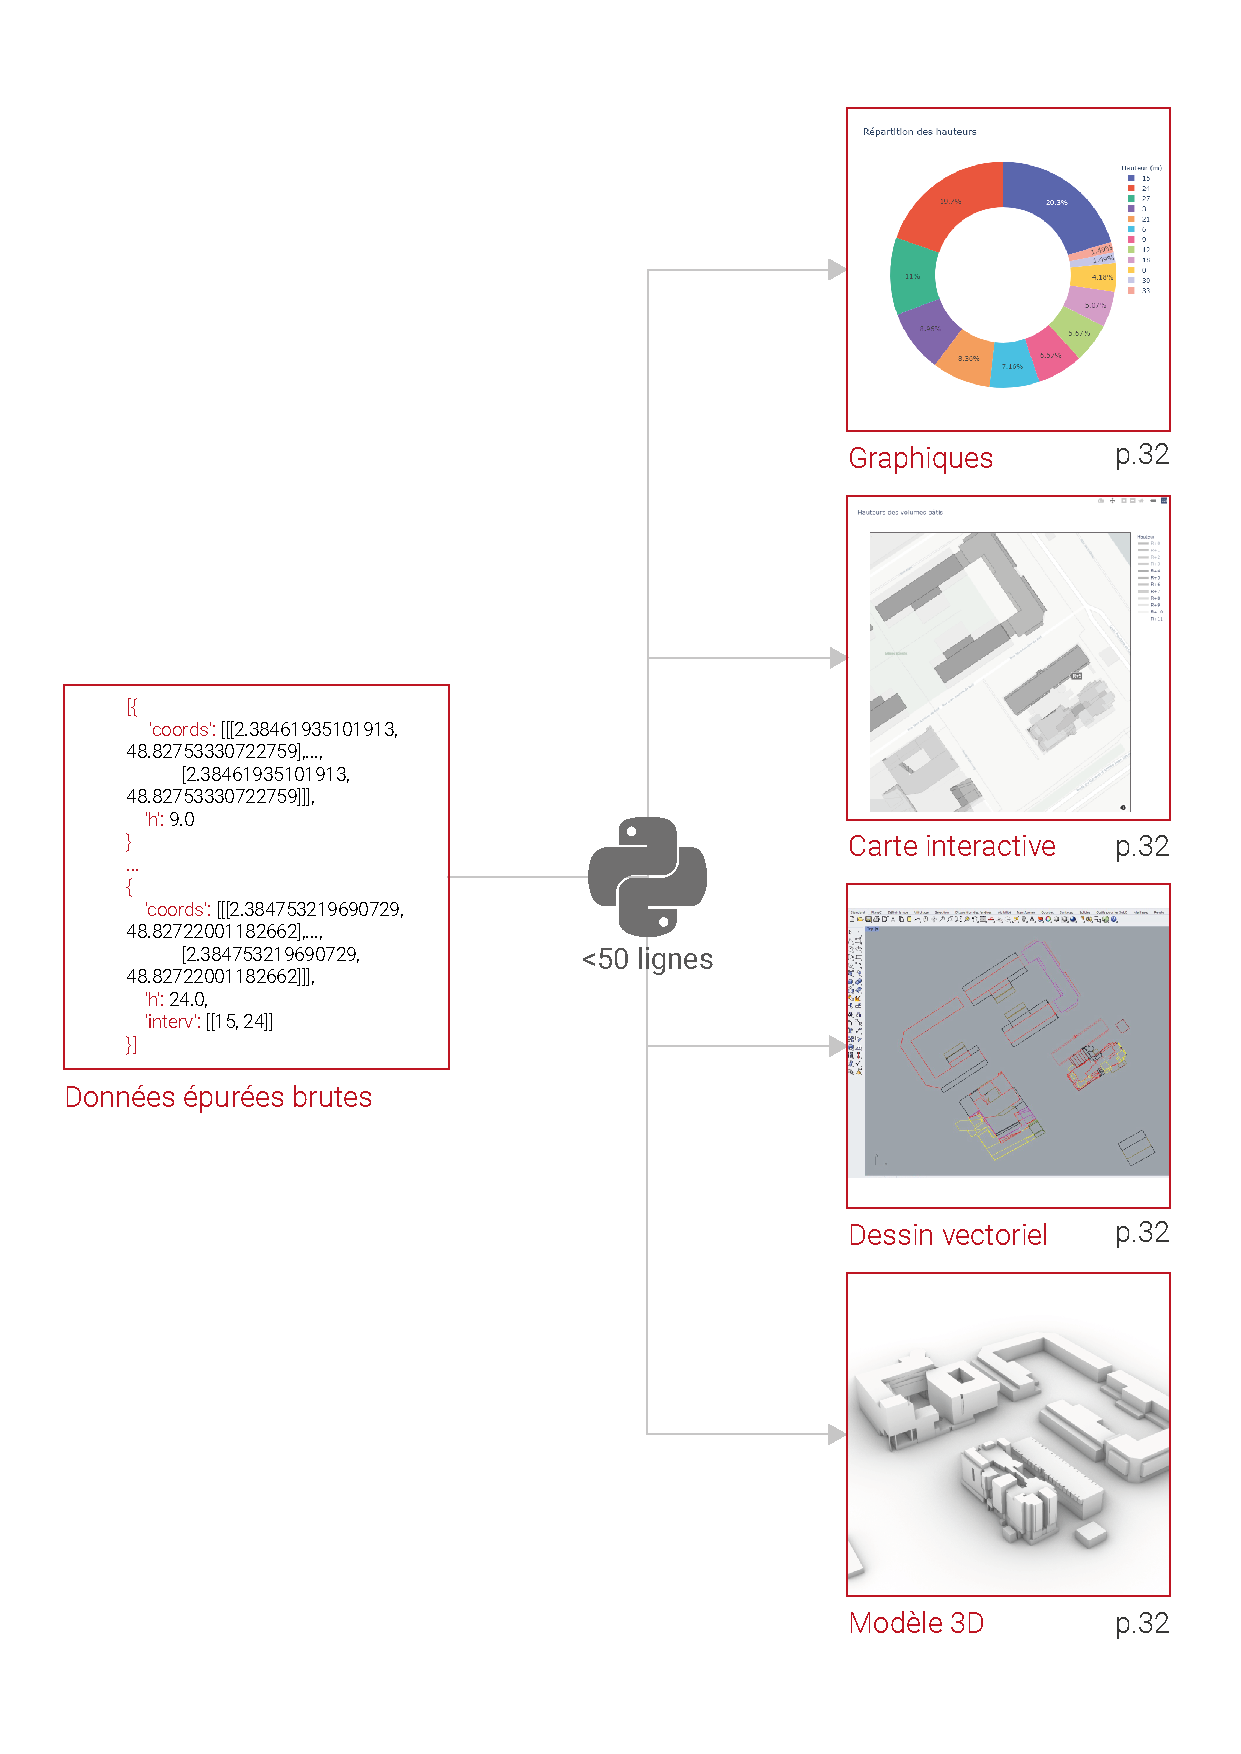
\includegraphics[height=1\textheight]{__imgs/p2} 

}

\caption[Moyens d'export et de synthèse des données récoltées  -  Réalisation personnelle]{Moyens d'export et de synthèse des données récoltées}\label{fig:p2_sommaire}
\end{figure}
\end{tcolorbox}

\newpage

\hypertarget{production-de-documents-synthuxe9tiques-interactifs}{%
\subsection{Production de documents synthétiques
interactifs}\label{production-de-documents-synthuxe9tiques-interactifs}}

Cette section présentera deux méthodes afin de visualiser les données
extraites. Au sein de cette section, la bibliothèque \emph{Plotly} sera
employée, possédant davantage d'options graphiques ainsi que de
possibilités d'export (dont des options d'interactivité) que son
concurrent plus répandu \emph{Matplotlib} mentionné précédemment.

\hypertarget{visualisation-statistique-des-donnuxe9es}{%
\subsubsection{Visualisation statistique des
données}\label{visualisation-statistique-des-donnuxe9es}}

Lorsque l'on aborde la question de la synthèse de données quelles
qu'elles soient, la représentation statistique par des graphiques semble
représenter l'approche la plus intuitive et la plus directe. Le premier
graphique créé sera un histogramme de \textbf{répartition du nombre de
volumes par hauteur}.

\begin{tcolorbox}[title= Moyens d'export et de synthèse des données récoltées ,colback=boitecode]
\begin{lstlisting}[style=code]
import plotly.graph_objects as go
n_par_hauteur = data["hauteur"].value_counts().to_dict()
print(n_par_hauteur)\end{lstlisting}

```
ttvar{#}ttvar{#} {18.0: 68, 27.0: 66, 30.0: 37, 6.0: 30, 24.0: 28, 9.0: 24, 12.0: 22, 15.0: 19, 21.0: 17, 3.0: 14, 33.0: 5, 36.0: 5}
```

\end{tcolorbox}

Le code ci-dessus permet d'importer la bibliothèque \emph{Plotly} (par
l'intermédiaire d'un de ses « sous-module » nommé « graph\_objects »,
que nous appellerons ici avec « go » tout au long du script). Après cet
import, la fonction \emph{value\_counts()} de \emph{GeoPandas} permet
ici de récupérer le \textbf{nombre de volumes par hauteur}
automatiquement (en énumérant chaque valeur possible et le nombre
d'occurrences dans la colonne), puis ajoute le tout dans un dictionnaire
nommé \textbf{n\_par\_hauteur}.\\
~\\
Enfin, quelques lignes de codes permettent à la fois la construction du
graphique, ainsi que son export. La \textbf{liste des différentes
hauteurs} (soit celle des \emph{attributs} du dictionnaire
\textbf{n\_par\_hauteur}) représentera l'axe \emph{x}, tandis que les
différents \textbf{nombres de volumes} associés formeront les valeurs à
renseigner pour l'axe \emph{y}. Quelques paramètres graphiques servent à
définir un titre général, des libellés pour les deux axes ainsi qu'une
résolution d'export. Ici, deux exports possibles seront montrés, à
savoir un export \textbf{statique} sous forme d'image au format PNG,
ainsi qu'un export \textbf{interactif} au sein d'une page web au format
HTML.

\begin{tcolorbox}[title= Moyens d'export et de synthèse des données récoltées ,colback=boitecode]
\begin{lstlisting}[style=code]
fig = go.Figure([go.Bar(x=list(n_par_hauteur.keys()), y=list(n_par_hauteur.values()),opacity=0.8,marker_color='rgb(200,0,0)')])
fig.update_xaxes(categoryorder='category ascending',tickvals=sorted(list(n_par_hauteur.keys())))\end{lstlisting}
\begin{lstlisting}[style=code]
fig.update_layout(title="Répartition des hauteurs",xaxis_title="hauteur (m)",yaxis_title="nombre de volumes",width=600,height=600)\end{lstlisting}
\begin{lstlisting}[style=code]
fig.write_image("OUTPUT/graphique_hauteurs.png")
fig.write_html("OUTPUT/graphique_hauteurs.html")\end{lstlisting}
\end{tcolorbox}

\begin{tcolorbox}
\begin{figure}

{\centering 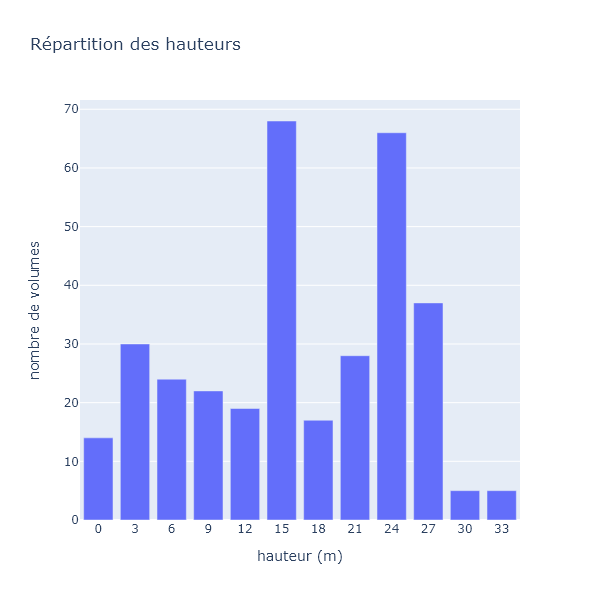
\includegraphics[width=0.45\linewidth]{OUTPUT/graphique_hauteurs} 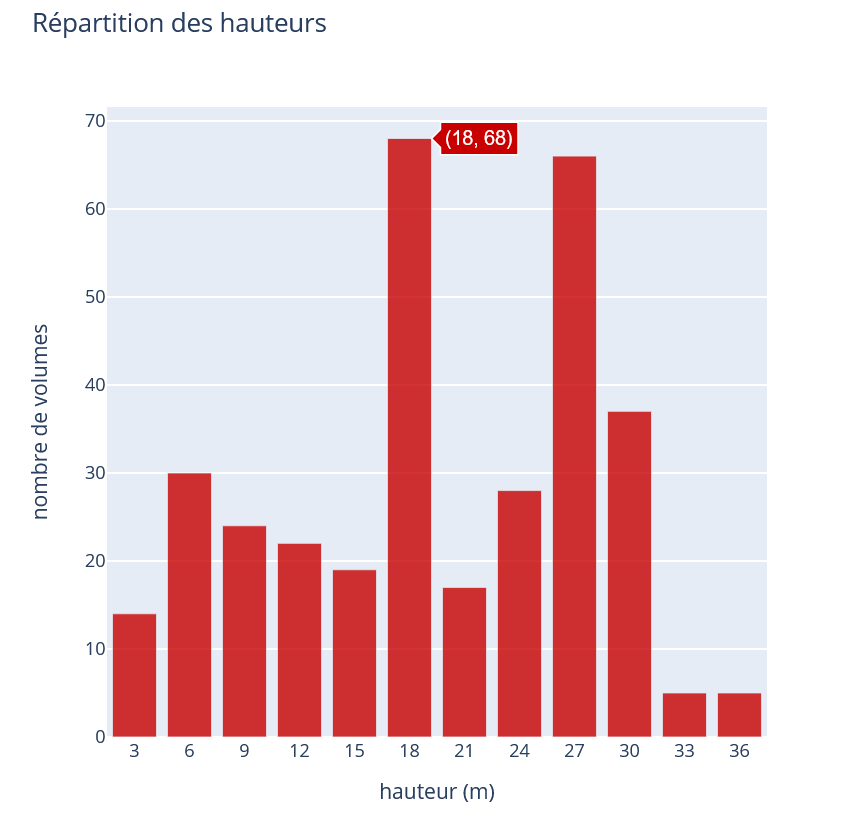
\includegraphics[width=0.45\linewidth]{__imgs/graphique_hauteurs_int} 

}

\caption[Nombre de volumes par hauteur  -  Réalisation personnelle]{Nombre de volumes par hauteur}\label{fig:graph_h}
\end{figure}
\end{tcolorbox}

Il est également possible de créer de la même manière une multitude
d'autres graphiques que \emph{Plotly} permet de construire. Un second
graphique plus complet peut être construit, en s'intéressant cette
fois-ci à une répartition \textbf{des volumes suivant leur hauteur, leur
surface et s'ils sont en porte à faux}. Ici, le sous-module
\emph{express} de \emph{Plotly} sera employé permettant une mise en
forme plus condensée. L'objectif est donc ici de se baser directement
sur le jeu de données des volumes. Cependant, une nouvelle colonne devra
être ajoutée, spécifiant si chaque volume est en porte à faux ou pas,
afin de pouvoir ajouter cette valeur dans \emph{Plotly}.

\begin{tcolorbox}[title= Nombre de volumes par hauteur ,colback=boitecode]
\begin{lstlisting}[style=code]
import plotly.express as px
# Fonction permettant de déterminer
# si un volume est en porte à faux
def is_paf(volume):
    if volume["hauteur_paf"] == None:
        return 0
    else:
        return 1

# Suppression de la colonne "geometry"
df = data.drop("geometry",axis=1)
# Création de la nouvelle colonne grâce à .apply()
df["is_paf"] = df.apply(lambda row : is_paf(row), axis=1)
# Génération du graphique et export
fig2 = px.parallel_coordinates(df, color="hauteur",color_continuous_scale=px.colors.sequential.amp)
fig2.update_layout(font={"size":20},width=1800,height=800)\end{lstlisting}
\begin{lstlisting}[style=code]
fig2.write_image("OUTPUT/graphique_repart.png")
fig2.write_html("OUTPUT/graphique_repart.html")\end{lstlisting}
\end{tcolorbox}

\begin{tcolorbox}
\begin{figure}

{\centering 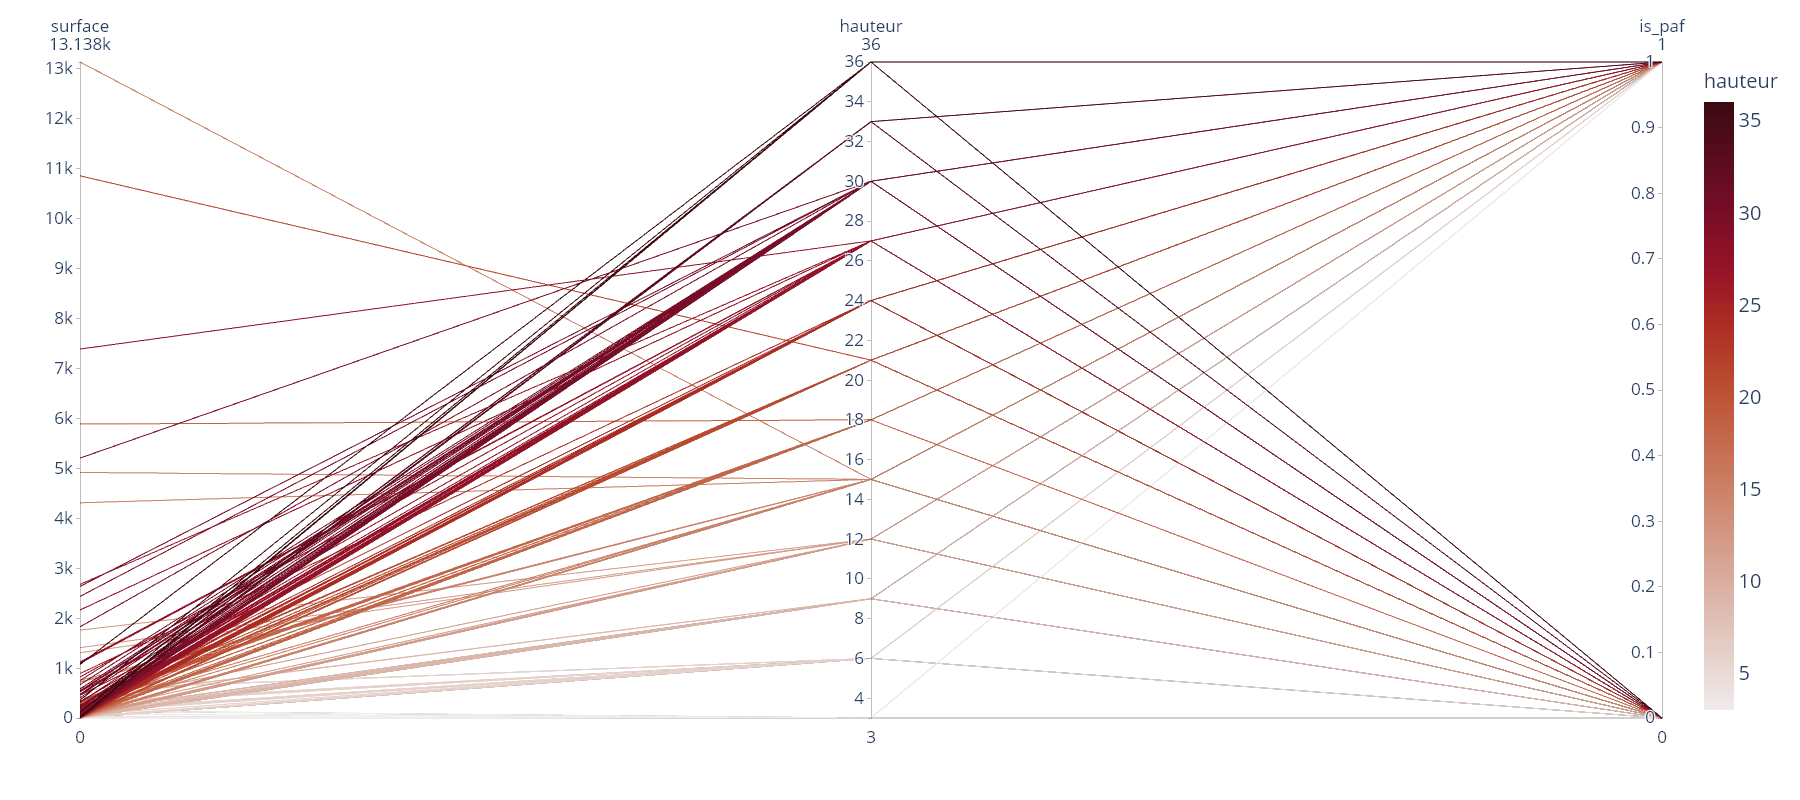
\includegraphics[width=0.9\linewidth]{OUTPUT/graphique_repart} 

}

\caption[Répartition des volumes selon leurs caractéristiques  -  Réalisation personnelle]{Répartition des volumes selon leurs caractéristiques}\label{fig:graph_repart}
\end{figure}
\end{tcolorbox}

En l'occurrence, le jeu de données extrait contient davantage de petites
surfaces ainsi qu'un nombre équlibré de volumes en porte à faux.
Cependant, cette souplesse dans la création de représentations
graphiques que permet \emph{Plotly} rend également possible de dessiner
les \textbf{emprises des volumes en eux-mêmes}, qui sera également
augmentée avec de l'interactivité.

\hypertarget{cartographier-de-maniuxe8re-interactive}{%
\subsubsection{Cartographier de manière
interactive}\label{cartographier-de-maniuxe8re-interactive}}

Cette sous-section a pour but de présenter une fonctionnalité
particulièrement utile pour la profession architecturale. En effet,
\emph{Plotly} est capable de créer de représenter des \textbf{formes
géométriques sur un fond de carte} (d'une manière similaire aux
solutions de SIG sans avoir besoin de convertir les coordonnées en
latitude/longitude), avec laquelle il est possible d'\textbf{interagir},
à travers notamment des fonctionnalités telles que le \textbf{zoom},
l'\textbf{affichage/masquage} d'élements légendés ainsi que l'affichage
de caractéristiques au \textbf{survol avec le curseur}. Ainsi,
l'objectif sera ici de générer une \textbf{carte interactive des volumes
par hauteur}.

\begin{tcolorbox}[title= Répartition des volumes selon leurs caractéristiques ,colback=boitecode]
\begin{lstlisting}[style=code]
import plotly.graph_objects as go
# Création de sous-groupes de volumes par hauteur
volumes_par_hauteur = data.groupby("hauteur")\end{lstlisting}
\end{tcolorbox}

Après avoir chargé le jeu de données de base, la première étape est de
\textbf{grouper les volumes par hauteur}. Ceci sera effectué grâce à la
fonction \emph{groupby()} de \emph{GeoPandas}. Le tout sera trié selon
la hauteur par \textbf{ordre croissant}.

Ensuite, une \textbf{boucle} en \textbf{for} permet d'itérer à travers
chaque groupe de \textbf{hauteur et ses volumes} afin de les tracer. Une
\textbf{couleur} sera préalablement attribuée pour chacune d'entre
elles, calculées selon une échelle de gris en RGB (plus le volume est
\textbf{haut}, plus il sera \textbf{clair}). La seule subtilité ici est
de devoir traiter \textbf{les listes de coordonnées latitude/longitude}
en \textbf{deux listes séparées}, et ainsi avoir une liste pour les
valeurs de \textbf{latitude} et une autre pour les valeurs de
\textbf{longitude}, contenant des valeurs \textbf{nulles} pour séparer
les volumes lors du traçage.\\

\begin{tcolorbox}[title= Répartition des volumes selon leurs caractéristiques ,colback=boitecode]
\begin{lstlisting}[style=code]
# Liste accueillant les couches de la carte
traces = []
for h,volumes in volumes_par_hauteur:
  couleur = "rgb(" + ",".join([str(h/max(data["hauteur"])*255)]*3) +")"
  X = []
  Y = []
  for geom in volumes["geometry"]:
    coords = geom.exterior.coords.xy
    X += list(coords[0][:-1])+[None] # longitude
    Y += list(coords[1][:-1])+[None] # latitude
    # Traçage des volumes
  print(X)
  traces.append(go.Scattermapbox(
    name=str(h) +"m",
    mode="lines",
    line = {"width" : 0.5, "color" : couleur},
    lon=X,
    lat=Y,
    opacity=1.0,
    hoverinfo="name",
    fill="toself"))\end{lstlisting}

```
ttvar{#}ttvar{#} [2.38359472591027, 2.383599407822562, 2.383314638116635, 2.383309851405566, None, 2.383130187598818, 2.383219065127394, 2.383064546641335, 2.383037750380318, 2.3830180134881322, None, 2.383373999467965, 2.3834458434070243, 2.38336763938613, 2.38326914275586, 2.383139956813265, 2.383343089516914, None, 2.383553338542729, 2.38359472591027, 2.383309851405566, 2.383268247172884, None, 2.383394344653911, 2.383399642873991, 2.383114982278648, 2.383109634847652, None, 2.383053285571433, 2.383061439915417, 2.382860958017709, 2.382852755378957, None, 2.382612428131992, 2.382653720199511, 2.3823657252506, 2.382324157221448, None, 2.385491575743618, 2.385569027588909, 2.385193405815913, 2.385115953543015, None, 2.382653720199511, 2.382658210783651, 2.382369499139243, 2.3823657252506, None, 2.384706806445656, 2.384740958806962, 2.384682795582728, 2.384648307654812, None, 2.385133069049484, 2.385144622244565, 2.385146850499722, 2.38517596420945, 2.385146747838012, 2.385112237722281, 2.385037743759729, 2.385070878083894, 2.384953293985822, 2.384920814855553, 2.384948817338635, 2.38493013983904, 2.384927324107389, 2.384960225463158, 2.384969185375871, 2.385063949715531, 2.385079311746132, 2.385100990200574, 2.385103233870903, None, 2.383399642873991, 2.383441502159596, 2.38315713460345, 2.383114982278648, None, 2.386052357186005, 2.386240262879141, 2.38627980451916, 2.386277017050273, 2.386160019293605, 2.386157996953355, 2.386116105304226, 2.386110060026099, 2.3860978642359543, 2.38609590265644, 2.3860447459333702, None, 2.382981647751976, 2.382992626663833, 2.382936058517719, None]
ttvar{#}ttvar{#} [2.38351222440612, 2.383527749099538, 2.383165045737739, 2.383149529111281, None, 2.3835074646454872, 2.38351222440612, 2.383149529111281, 2.383144772055544, None, 2.384793138774722, 2.384819249502677, 2.384796971933453, 2.384770481308271, None, 2.38447966711214, 2.384487634491064, 2.384491575487986, 2.384484774564641, 2.384480825171988, 2.384472872701151, None, 2.382852755378957, 2.382860958017709, 2.382772819795223, 2.382768801443258, 2.382758597346497, None, 2.384345535850388, 2.384353569470516, 2.384349127917778, 2.384341172862691, None, 2.385024389584457, 2.385037872116996, 2.385035387981625, 2.385020911192861, 2.385007479473476, None, 2.385160753936447, 2.385174401636668, 2.385156579986841, 2.385143057055164, 2.385157753204874, None, 2.382837184858754, 2.382882167483829, 2.382749461588344, 2.3827045846637143, None, 2.38357810709207, 2.383637277091971, 2.383498247318974, 2.383448092442052, 2.383563150985368, None, 2.38456873270404, 2.384553506023605, 2.384391371394361, 2.384388178992803, 2.384405302707107, 2.384442505685409, 2.384479558347809, 2.3845163997295202, 2.384552118245864, None, 2.383576229825127, 2.383619021266707, 2.383617114397362, 2.383349583935744, 2.383306315872272, None, 2.383599407822562, 2.383644567365891, 2.383359916720667, 2.383314638116635, None, 2.385430403330743, 2.385491575743618, 2.385115953543015, 2.385054780792404, None, 2.384575654685379, 2.384592041213091, 2.384586015415385, 2.384581597086672, 2.384577439054112, 2.384575044805671, 2.384573845038873, 2.384576016445481, 2.384554935749008, 2.384524821022413, 2.384537906035579, 2.384525472540164, 2.384530155210721, 2.38454240310143, 2.384575456845994, 2.384571024584386, None, 2.3845126856021253, 2.384524821022413, 2.3845183543743262, 2.384506304318764, None, 2.382658210783651, 2.3827045846637143, 2.382415987747675, 2.382369499139243, None, 2.384380749961067, 2.384388744344044, 2.384384151074258, 2.384376185146007, None, 2.384459896135067, 2.384468034160981, 2.38446318758718, 2.384455244607229, None, 2.383918111832674, 2.383961321237744, 2.383956745150472, 2.383913883984746, None, 2.382723372291977, 2.382731582272882, 2.382783687081833, 2.382800331545297, 2.3828892079809663, 2.382881039898677, 2.382832802026658, 2.38279386647823, 2.382737921495009, 2.382711719476917, 2.382632760642688, 2.382571608110008, None, 2.384591275760087, 2.384597659243542, 2.384604096304909, 2.3846147562394, 2.384622830912725, 2.384629481798523, 2.384636766433263, 2.384644105454289, 2.384648307654812, 2.384682795582728, 2.384678279706455, 2.3846856046224643, 2.384671033497087, 2.384669042167505, 2.384632412100034, 2.384570429741702, None, 2.383349583935744, 2.383394344653911, 2.383109634847652, 2.383064721909355, None, 2.383020921093123, 2.383064721909355, 2.382793264264163, 2.382790951264449, 2.38274956243521, None, 2.383359916720667, 2.383403039646997, 2.383268846948252, 2.383225799515196, None, 2.383913883984746, 2.383956745150472, 2.383687670510199, 2.383644567365891, None, 2.3834219386721163, 2.383562572673297, 2.383547627811939, 2.383563150985368, 2.383448092442052, 2.3834458434070243, 2.383373999467965, 2.383525544462175, 2.383471416748627, 2.383457343016415, 2.383401667956741, None, 2.384422326404447, 2.384430285604047, 2.38442184947827, 2.384413707426916, None, 2.385569027588909, 2.385630199628913, 2.385254578193654, 2.385193405815913, None, 2.385084569352983, 2.385114270227686, 2.385111357913541, 2.385106894616643, 2.385077653322637, 2.385081991754463, None]
ttvar{#}ttvar{#} [2.384339374613817, 2.38436317076471, 2.384354616621883, 2.38435287869225, 2.384329056412861, 2.384330650600268, None, 2.384799823694364, 2.384804777119808, 2.384765083435587, 2.384767561203148, 2.3846906191480333, 2.3846856046224643, 2.3847522915575903, 2.384749621781722, None, 2.384750690625121, 2.384769676371753, 2.384757010854756, 2.384751917314584, 2.384748259198208, 2.384745757323124, None, 2.384695771780973, 2.384702507681742, 2.384707146202921, 2.384438357897507, 2.384421287166987, 2.3844241303670453, 2.384426095462247, 2.384437534538122, 2.384448066458244, 2.384457581915215, 2.384458906619311, 2.384493300954779, 2.3845760612940152, 2.384597148193879, 2.384670736411505, 2.384693506417872, 2.384691603834422, None, 2.384484774564641, 2.384584367034765, 2.38456873270404, 2.384552118245864, 2.384449021957285, 2.384467430353121, 2.38446318758718, 2.384468034160981, 2.384472105950347, None, 2.3847885280801, 2.384827301163695, 2.384819249502677, 2.384793138774722, 2.384770481308271, 2.384753693359777, None, 2.384354616621883, 2.384366938720035, 2.384357745769514, 2.384345229414283, 2.38435287869225, None, 2.384435547915448, 2.384437534538122, 2.384426095462247, 2.3844241303670453, None, 2.384449021957285, 2.384552118245864, 2.3845163997295202, 2.384413806812996, 2.384426142815591, 2.38442184947827, 2.384430285604047, 2.384434379514246, None, 2.3843178794105873, 2.384330650600268, 2.384329056412861, 2.384321837201008, 2.384308693011729, None, 2.384669042167505, 2.384671033497087, 2.384676042093934, 2.384673792276123, 2.384709856371621, 2.384682097365824, 2.384671978633884, 2.384665028054613, 2.384632412100034, None, 2.384413806812996, 2.3845163997295202, 2.384479558347809, 2.384376415412893, 2.384388342638891, 2.384384151074258, 2.384388744344044, 2.38439293842034, None, 2.384376415412893, 2.384479558347809, 2.384442505685409, 2.384339470384334, 2.38435313230774, 2.384349127917778, 2.384353569470516, 2.384357727411771, None, 2.385116034407233, 2.385215915296804, 2.385098320466351, 2.384998439467982, None, 2.384339470384334, 2.384442505685409, 2.384405302707107, 2.384302044396005, None, 2.3846856046224643, 2.3846906191480333, 2.384676042093934, 2.384671033497087, None, 2.385077653322637, 2.385106894616643, 2.385078318681242, 2.385048676681234, None, 2.384827301163695, 2.3848314162145012, 2.384823342166308, 2.384819249502677, None, 2.383637277091971, 2.383637945254208, 2.383498915471622, 2.383498247318974, None, 2.384302044396005, 2.384405302707107, 2.384388178992803, 2.384386577960863, 2.384391899895742, 2.384388135312407, 2.384393244756017, 2.384368225956252, 2.384363077441777, 2.384359073038587, 2.384354002988808, 2.3843489323828, 2.384345821050986, 2.384278018365455, 2.384280873742134, 2.38428489047819, None, 2.384758393289523, 2.384762919592936, 2.384753219690729, 2.38474889473712, None, 2.383527749099538, 2.383561294748624, 2.383198575252582, 2.383165045737739, None, 2.384342055068027, 2.384366027565814, 2.38436317076471, 2.384339374613817, None, 2.385112237722281, 2.385146747838012, 2.385134837066289, 2.385123788871553, 2.385110819455202, 2.385093407539174, 2.385070878083894, 2.385037743759729, None]
ttvar{#}ttvar{#} [2.38461935101913, 2.384628217027156, 2.3846363958367522, 2.384645732926233, 2.384652326040948, 2.384656649382123, 2.3846610231503442, 2.38466170017297, 2.3846595300456173, 2.3846568869734233, 2.384651922306437, 2.384644105454289, 2.384636766433263, 2.384629481798523, 2.384622830912725, 2.3846147562394, 2.384604096304909, 2.384597659243542, 2.384591275760087, 2.384570429741702, 2.384564292829435, 2.384626028289865, 2.384605980177239, 2.384599619398239, 2.384590133231389, 2.384491575487986, 2.384502471066941, 2.384490396493715, 2.384495045310945, 2.38450719147041, 2.3845183543743262, 2.384548210954412, 2.384554935749008, 2.384576016445481, 2.384573845038873, 2.384575044805671, 2.384577439054112, 2.384581597086672, 2.384586015415385, 2.384592041213091, 2.384603039948636, 2.384612013974757, None, 2.384632412100034, 2.384665028054613, 2.384646985809988, 2.384642599218182, 2.384605980177239, 2.384626028289865, None, 2.384770481308271, 2.384796971933453, 2.384782602464847, 2.384756236578184, None, 2.384069000600689, 2.3841101866456382, 2.384104421076627, 2.384063553219252, None, 2.3847772780421073, 2.384786061081445, 2.384774750962177, 2.384792460243811, 2.384709856371621, 2.384673792276123, 2.384676042093934, 2.384685659918919, 2.384700376947829, None, 2.384524821022413, 2.384554935749008, 2.384548210954412, 2.3845183543743262, None, 2.383457343016415, 2.383471416748627, 2.38346805263632, 2.383453909799568, None, 2.384570429741702, 2.384632412100034, 2.384626028289865, 2.384564292829435, None, 2.384490396493715, 2.384502471066941, 2.384491575487986, 2.384487634491064, 2.38447966711214, None, 2.384753693359777, 2.384770481308271, 2.384756236578184, 2.384782602464847, 2.384777832964309, 2.384776165069041, 2.384773740921274, 2.384755025302945, 2.384739325132708, 2.384730213469595, 2.38471745135964, None, 2.3830180134881322, 2.383037750380318, 2.382992626663833, 2.382981647751976, None, 2.3846906191480333, 2.384700376947829, 2.384685659918919, 2.384676042093934, None, 2.384063553219252, 2.384104421076627, 2.38341606121346, 2.38337592773961, None, 2.384796971933453, 2.384805644256796, 2.38481845937626, 2.384831452192506, 2.384770285503551, 2.384762919592936, 2.384798454750741, 2.384782602464847, None, 2.382982249009329, 2.383025468598765, 2.382329784196446, 2.382285859369545, None, 2.384767561203148, 2.3847772780421073, 2.384700376947829, 2.3846906191480333, None, 2.384491575487986, 2.384590133231389, 2.384584367034765, 2.384484774564641, None, 2.383001384700814, 2.383019920729644, 2.3830065853845213, None, 2.383001384700814, 2.383028180962984, 2.383019920729644, None, 2.384755025302945, 2.384773740921274, 2.384776165069041, 2.384777832964309, 2.384782602464847, 2.384798454750741, 2.384762919592936, 2.384758393289523, 2.384757010854756, 2.384769676371753, 2.384750690625121, 2.384745757323124, 2.384742770046282, 2.384739325132708, None, 2.384506304318764, 2.3845183543743262, 2.38450719147041, 2.384495045310945, None, 2.383429522701743, 2.383474270291981, 2.3826484968823243, 2.382602927603132, None]
ttvar{#}ttvar{#} [2.384546063428376, 2.384535168124212, 2.384542511367397, 2.384520482801822, 2.384516295838293, 2.384392922817853, None, 2.384553506023605, 2.384546063428376, 2.384392922817853, 2.384391371394361, None, 2.383956745150472, 2.384063553219252, 2.38337592773961, 2.383268846948252, 2.383403039646997, 2.383687670510199, None, 2.3827045846637143, 2.382749461588344, 2.382460844346099, 2.382415987747675, None, 2.384261183236321, 2.384277662936312, 2.384274891604106, 2.38425825710247, None, 2.384382277674946, 2.384392952879501, 2.384371090979606, 2.384383387169934, 2.3843787410512, 2.384366274668431, 2.384344465292466, 2.384333277962699, None, 2.383498915471622, 2.38350598832206, 2.383505750460362, 2.383498096788995, 2.383490440298251, 2.383482782371383, 2.383475120273679, 2.383467455377756, 2.383459787662446, 2.383455530350949, None, 2.382758597346497, 2.382768801443258, 2.382731582272882, 2.382723372291977, None, 2.383306315872272, 2.383349583935744, 2.383064721909355, 2.383020921093123, None, 2.38350598832206, 2.383521854698119, 2.38344511780431, 2.383431049252724, 2.383455530350949, 2.383459787662446, 2.383467455377756, 2.383475120273679, 2.383482782371383, 2.383490440298251, 2.383498096788995, 2.383505750460362, None, 2.383961321237744, 2.38396505054181, 2.384060934283225, 2.384069000600689, 2.384063553219252, 2.383956745150472, None, 2.384200695408299, 2.384447775991725, 2.384197245709779, None, 2.384311187884772, 2.384312401981532, 2.384261183236321, 2.38425825710247, 2.384274891604106, 2.384263975580174, 2.384245152238602, None, 2.382531951724662, 2.38263236015402, 2.382362867784657, 2.382075710455427, 2.381813974367699, 2.381859404586527, 2.382155867152994, 2.382200822656329, 2.382460844346099, 2.382749461588344, 2.382882167483829, 2.382982249009329, 2.382285859369545, 2.382280166169525, 2.382062501902879, 2.382058124944137, 2.3816582866463323, 2.381702403587981, 2.381698170300775, None, 2.383474270291981, 2.383478597008037, 2.383573481355076, 2.383576229825127, 2.383306315872272, 2.383020921093123, 2.38274956243521, 2.3826484968823243, None, 2.383575111760181, 2.383628941822758, 2.383561294748624, 2.383527749099538, 2.38351222440612, 2.3835074646454872, None, 2.383521854698119, 2.383575111760181, 2.3835074646454872, 2.38344511780431, None, 2.383644567365891, 2.383687670510199, 2.383403039646997, 2.383359916720667, None, 2.384691603834422, 2.384693506417872, 2.384670736411505, 2.384668525078728, None]
ttvar{#}ttvar{#} [2.384181633062092, 2.384194331499211, 2.384161356434451, 2.38414952242287, None, 2.384550966464224, 2.384563343579427, 2.384532866095999, 2.384520565555205, None, 2.384263760668778, 2.3842755980438213, 2.3842428289333473, 2.384230945525621, None, 2.384887948508663, 2.384889393768994, 2.384857687625145, 2.384853816296832, 2.384824393961787, 2.384819761376712, 2.384790773870481, 2.38478620495611, 2.384757268940267, 2.384752802974218, 2.384721542563063, 2.384712392551165, 2.384679422710442, 2.3846750380194432, 2.384644282908237, 2.384639766830195, 2.384609152599459, 2.384604503783152, 2.3845716667591272, 2.38457016906715, None, 2.383188696114628, 2.383189752219737, 2.3831746474096, 2.383172317773195, None, 2.384140299619068, 2.384152224089871, 2.3841193018954803, 2.384107084050585, None, 2.384032387882543, 2.384044765440499, 2.384011687521417, 2.384003506909771, 2.383999426238666, None, 2.384413707426916, 2.38442184947827, 2.384409634169658, 2.384388744344044, 2.384380749961067, None, 2.384216934261485, 2.38422947113855, 2.384198789313575, 2.384186537328904, None, 2.384376185146007, 2.384384151074258, 2.384372252738265, 2.384353569470516, 2.384345535850388, None, 2.383745823060639, 2.3837667644205, 2.383583825933569, 2.383564041340075, None, 2.382936058517719, 2.382992626663833, 2.383001384700814, 2.382931043032187, None, 2.384472872701151, 2.384480825171988, 2.384468034160981, 2.384459896135067, None, 2.384480947159016, 2.384492916244591, 2.384459927463976, 2.384447975205223, None, 2.384853816296832, 2.384865722505464, 2.384836431535653, 2.384824393961787, None, 2.384712392551165, 2.384724477281595, 2.384691758219886, 2.384679422710442, None, 2.384298035822527, 2.384302044396005, 2.38428489047819, 2.384280873742134, None, 2.384515767184888, 2.38452820914221, 2.384497429620997, 2.384485284272853, None, 2.384804919669021, 2.384814352008841, 2.384813222252019, 2.384848973460015, 2.3847692387780253, 2.384771826863573, 2.384743357630168, 2.384705373250871, 2.384707902115854, 2.384697900612702, 2.384722451532606, None, 2.382992626663833, 2.383037750380318, 2.383042951048965, 2.383028180962984, 2.383001384700814, None, 2.383037750380318, 2.383064546641335, 2.383042951048965, None, 2.384480825171988, 2.384484774564641, 2.384472105950347, 2.384468034160981, None, 2.384031573914393, 2.384127694135401, 2.384060934283225, 2.38396505054181, None, 2.384639766830195, 2.38465175932092, 2.384621266587493, 2.384609152599459, None, 2.384729235306871, 2.384741691374475, 2.3847127403872213, 2.384700337930158, None, 2.384752802974218, 2.384764701915612, 2.384733682076653, 2.384721542563063, None, 2.384197245709779, 2.384447775991725, 2.384417147518882, 2.384170734809704, None, 2.384331363101974, 2.384343514620379, 2.384310623458348, 2.384298699288176, None, 2.3846750380194432, 2.384686640996144, 2.384656747468889, 2.384644282908237, None, 2.384156537869262, 2.384168384907048, 2.384135717065859, 2.384123641511803, None, 2.384409634169658, 2.384413806812996, 2.38439293842034, 2.384388744344044, None, 2.384392952879501, 2.3844047701093842, 2.384383387169934, 2.384371090979606, None, 2.384455244607229, 2.38446318758718, 2.38444485105956, 2.384430285604047, 2.384422326404447, None, 2.384589120538808, 2.384600638564825, 2.384567714727955, 2.384555836709897, None, 2.38478620495611, 2.384798276949755, 2.384769549488314, 2.384757268940267, None, 2.384819761376712, 2.38483174125145, 2.384803062506585, 2.384790773870481, None, 2.382931043032187, 2.383001384700814, 2.38289969283395, 2.38292970583262, None, 2.383884933045907, 2.384132682184153, 2.38412768471406, 2.383875361860307, None, 2.383875361860307, 2.38412768471406, 2.38410212283339, 2.383853675936881, 2.38387213396469, None, 2.384782968891893, 2.384891964425352, 2.384894721249127, 2.384889393768994, 2.384887948508663, 2.38457016906715, 2.3845716667591272, 2.384562952932372, 2.384530155210721, 2.384525472540164, 2.3845126856021253, 2.384506304318764, 2.384495045310945, 2.384490396493715, 2.38447966711214, 2.384472872701151, 2.384459896135067, 2.384455244607229, 2.384422326404447, 2.384413707426916, 2.384380749961067, 2.384376185146007, 2.384345535850388, 2.384341172862691, 2.384272917384115, 2.384263760668778, 2.384230945525621, 2.384226616407837, 2.384195990223859, 2.384191879192763, 2.384161189361091, 2.384156537869262, 2.384123641511803, 2.384118012041759, 2.384006246334049, 2.384011687521417, 2.384044765440499, 2.384049078296857, 2.384079811531379, 2.384084198890629, 2.384114754689446, 2.3841193018954803, 2.384152224089871, 2.384161356434451, 2.384194331499211, 2.384198789313575, 2.38422947113855, 2.384233859871906, 2.384264423873618, 2.384268701545519, 2.384301596747337, 2.384310623458348, 2.384343514620379, 2.384348106550041, 2.384356488505315, 2.3843787410512, 2.384383387169934, 2.3844047701093842, 2.384414052848854, 2.384418387410861, 2.384451498085272, 2.384459927463976, 2.384492916244591, 2.384497429620997, 2.38452820914221, 2.384532866095999, 2.384563343579427, 2.384567714727955, 2.384600638564825, 2.384609613852328, 2.384640849934489, 2.384645483869733, 2.3846745323612, 2.38467915275267, 2.384708145724072, 2.3847127403872213, 2.384741691374475, 2.384746038157575, 2.384777652239684, 2.384781396237968, None, 2.3843969807179732, 2.384417576744092, 2.384235922517688, 2.384215145990781, None, 2.384366274668431, 2.3843787410512, 2.384356488505315, 2.384344465292466, None, 2.384103115427916, 2.384114754689446, 2.384084198890629, 2.384071957194108, None, 2.383549292385752, 2.38364502890231, 2.383573481355076, 2.383478597008037, None, 2.384344465292466, 2.384356488505315, 2.384348106550041, 2.384336027883727, None, 2.38444485105956, 2.384449021957285, 2.384434379514246, 2.384430285604047, None, 2.384341172862691, 2.384349127917778, 2.384335472740511, 2.384298035822527, 2.384280873742134, 2.384272917384115, None, 2.384349127917778, 2.38435313230774, 2.384339470384334, 2.384335472740511, None, 2.384191879192763, 2.384203857124744, 2.384172916208472, 2.384161189361091, None, 2.384067021231738, 2.384079811531379, 2.384049078296857, 2.3840367388604102, None, 2.3846622256857, 2.3846745323612, 2.384645483869733, 2.384633053824722, None, 2.384765456848367, 2.384777652239684, 2.384746038157575, 2.38473398774957, None, 2.38446318758718, 2.384467430353121, 2.384449021957285, 2.38444485105956, None, 2.384562952932372, 2.384571024584386, 2.384575456845994, 2.38454240310143, 2.384530155210721, None, 2.384695911603372, 2.384708145724072, 2.38467915275267, 2.384667145818654, None, 2.38442184947827, 2.384426142815591, 2.384413806812996, 2.384409634169658, None, 2.384226616407837, 2.384238951102482, 2.384207571745325, 2.384195990223859, None, 2.384439621915035, 2.384451498085272, 2.384418387410861, 2.384406322122525, None, 2.384251949926268, 2.384264423873618, 2.384233859871906, 2.384221218719346, None, 2.384289488089232, 2.384301596747337, 2.384268701545519, 2.384256412536554, None, 2.384335472740511, 2.384339470384334, 2.384302044396005, 2.384298035822527, None, 2.384384151074258, 2.384388342638891, 2.384376415412893, 2.384372252738265, None, 2.384372252738265, 2.384376415412893, 2.384357727411771, 2.384353569470516, None, 2.384604503783152, 2.384616635871397, 2.384583869880597, 2.3845716667591272, None, 2.384889393768994, 2.384901769289657, 2.384878760474949, 2.384869980125149, 2.384857687625145, None, 2.384401402885024, 2.384414052848854, 2.3844047701093842, 2.384392952879501, None, 2.384525472540164, 2.384537906035579, 2.384524821022413, 2.3845126856021253, None, 2.384628900176, 2.384640849934489, 2.384609613852328, 2.384597408594293, None]
ttvar{#}ttvar{#} [2.383058687224778, 2.383144772055544, 2.383149529111281, 2.383145945988593, 2.383054705950134, None, 2.382984494208129, 2.382997591727526, 2.383058687224778, 2.383054705950134, 2.382979919153169, None, 2.3837667644205, 2.383852432931372, 2.383853675936881, 2.38410212283339, 2.384170734809704, 2.384417147518882, 2.3843969807179732, 2.384215145990781, 2.384165437028186, 2.384154133440184, 2.384127694135401, 2.384031573914393, 2.384149332037207, 2.384179787930417, 2.3840532860167603, 2.384022288216069, 2.383884149462545, 2.383914575113517, 2.383792295604149, 2.383760560858792, 2.38364502890231, 2.383549292385752, 2.383523908956134, 2.383536359581687, 2.383583825933569, None, 2.3840532860167603, 2.384179787930417, 2.384149332037207, 2.384022288216069, None, 2.382881039898677, 2.382883368158811, 2.382835141290822, 2.382832802026658, None, 2.382974390433356, 2.382984494208129, 2.382979919153169, 2.382971033162084, None, 2.382832802026658, 2.382835141290822, 2.382801185929213, 2.382731672547854, 2.38272934427373, 2.38273270146399, 2.382737921495009, 2.38279386647823, None, 2.383792295604149, 2.383914575113517, 2.383884149462545, 2.383760560858792, None, 2.383637945254208, 2.383665758552279, 2.3836581706222413, 2.383650579883418, 2.383642984973819, 2.383635388628153, 2.383627786749616, 2.383620183424374, 2.383612575928345, 2.383604965623514, 2.383597352520614, 2.383589735246817, 2.383582115164313, 2.383574492273098, 2.3835668665837, 2.383559238085485, 2.383551605416459, 2.383543969938612, 2.383536333024761, 2.383528691929358, 2.383521046673769, 2.383513399971434, 2.38350598832206, 2.383498915471622, None, 2.3828892079809663, 2.382934112450155, 2.3829727647095362, 2.382974390433356, 2.382971033162084, 2.382928987956231, 2.3828879690602323, 2.382883368158811, 2.382881039898677, None, 2.383149529111281, 2.383165045737739, 2.383161463967014, 2.383145945988593, None, 2.383679058337889, 2.383767522287959, 2.383744949262097, 2.383691119269245, 2.383575111760181, 2.383521854698119, None, 2.383665758552279, 2.383679058337889, 2.383521854698119, 2.38350598832206, 2.383513399971434, 2.383521046673769, 2.383528691929358, 2.383536333024761, 2.383543969938612, 2.383551605416459, 2.383559238085485, 2.3835668665837, 2.383574492273098, 2.383582115164313, 2.383589735246817, 2.383597352520614, 2.383604965623514, 2.383612575928345, 2.383620183424374, 2.383627786749616, 2.383635388628153, 2.383642984973819, 2.383650579883418, 2.3836581706222413, None, 2.383668440308428, 2.383769911966136, 2.383767522287959, 2.383679058337889, 2.383665758552279, None, 2.38364034183125, 2.383668440308428, 2.383665758552279, 2.383637945254208, None, 2.383628941822758, 2.383631282431362, 2.3835137223140013, 2.383197331400254, 2.383162359456629, 2.383161463967014, 2.383165045737739, 2.383198575252582, 2.383561294748624, None, 2.383691119269245, 2.383744949262097, 2.383628941822758, 2.383575111760181, None]
ttvar{#}ttvar{#} [2.3828879690602323, 2.382884727932288, 2.382883368158811, None, 2.383631282431362, 2.383649595432706, 2.383573502167259, 2.383540486577307, 2.3835137223140013, None, 2.383453909799568, 2.38346805263632, 2.383453477074585, 2.383439403339944, None, 2.384328985176413, 2.384342055068027, 2.384339374613817, 2.384326383127431, None, 2.382979919153169, 2.383054705950134, 2.383038822949116, 2.383031577109533, 2.382977788098112, None, 2.383162359456629, 2.383197331400254, 2.3831588833415083, None, 2.383054705950134, 2.383145945988593, 2.383161463967014, 2.383157907969227, 2.383038822949116, None, 2.384642599218182, 2.384646985809988, 2.384618480444647, None, 2.384854650885232, 2.384866601675864, 2.384885465101338, 2.384909938740101, 2.384893814076154, 2.38485481620255, 2.384850126212675, 2.384848973460015, 2.384813222252019, 2.384814352008841, None, 2.385048676681234, 2.385078318681242, 2.385032848613459, 2.385027663806182, 2.385006424510293, 2.384986424406501, 2.38500796730982, 2.385003499000548, None, 2.384665028054613, 2.384675067209857, 2.384628852354815, 2.384618480444647, 2.384646985809988, None, 2.383573502167259, 2.383544389293664, 2.383540486577307, None, 2.3829527622865703, 2.382966675389694, 2.382948051624978, None, 2.382835141290822, 2.382850770815224, 2.382850509821516, 2.382844799851887, 2.382731672547854, 2.382801185929213, None, 2.383161463967014, 2.383162359456629, 2.3831588833415083, 2.383157907969227, None, 2.3828879690602323, 2.382928987956231, 2.382971033162084, 2.382966675389694, 2.3829527622865703, 2.382927308402034, 2.382894289665835, 2.3828908200115873, 2.382887136107441, None, 2.382883368158811, 2.382884727932288, 2.382850770815224, 2.382835141290822, None, 2.384671978633884, 2.384682097365824, 2.384675067209857, 2.384665028054613, None, 2.384705373250871, 2.384743357630168, 2.384771826863573, 2.3847885280801, 2.384753693359777, 2.38471745135964, 2.3847082977459, 2.384710329513138, 2.384619552091428, 2.384576505868194, 2.3845373712546323, 2.384594019139818, 2.38459119330945, 2.384632826284968, 2.384621445262769, None, 2.382887136107441, 2.3828908200115873, 2.382894289665835, 2.382927308402034, 2.3829527622865703, 2.382948051624978, 2.382903541224776, 2.382883964431776, None, 2.382971033162084, 2.382979919153169, 2.382977788098112, None, 2.384366027565814, 2.384378466803838, 2.384375537034999, 2.38436317076471, None, 2.384682959163031, 2.384695771780973, 2.384691603834422, 2.384668525078728, 2.384659106934159, 2.384655901471765, None, 2.3835137223140013, 2.383540486577307, 2.383509868778753, 2.383498424610402, 2.383197331400254, None, 2.384326383127431, 2.384339374613817, 2.384330650600268, 2.3843178794105873, None, 2.384383532409021, 2.384407841976056, 2.384366027565814, 2.384342055068027, None, 2.38436317076471, 2.384375537034999, 2.384366938720035, 2.384354616621883, None, 2.383540486577307, 2.383544389293664, 2.383498424610402, 2.383509868778753, None]
ttvar{#}ttvar{#} [2.384753219690729, 2.384761632106771, 2.384739182508318, 2.3847246454617173, 2.384721921583155, None, 2.383544389293664, 2.38323499859472, 2.383220170085687, 2.383498424610402, None, 2.383038822949116, 2.383157907969227, 2.383153687424757, 2.3830385512817402, None, 2.385004697826526, 2.385007479473476, 2.385004759545134, 2.385003607417802, 2.384969997321697, 2.384953662980202, 2.384799823694364, 2.384798411768039, 2.384829778604734, 2.384822549336548, 2.384868785492021, 2.384878437072628, 2.384890050069025, 2.384902915781311, 2.384914979717119, 2.384953439030514, 2.384969966084438, 2.385000255287443, None, 2.382966675389694, 2.382971033162084, 2.382969901905299, None, 2.384710329513138, 2.384733123337365, 2.384702955946621, 2.384701340360203, 2.384651905233463, 2.384636957772319, 2.384619552091428, None, 2.384587728413743, 2.384592594894788, 2.38458547288516, 2.384583861957639, 2.384553506023605, 2.38456873270404, None, 2.383220170085687, 2.38323499859472, 2.3832179493656582, None, 2.383157907969227, 2.3831588833415083, 2.383154617859806, 2.383153687424757, None, 2.384739325132708, 2.384742770046282, 2.384745757323124, 2.384748259198208, 2.384751917314584, 2.384757010854756, 2.384758393289523, 2.38474889473712, 2.384753219690729, 2.384721921583155, 2.384714194969687, 2.3847206900263203, 2.384705785702895, 2.384742342482762, 2.3847348404737803, 2.384733123337365, None, 2.382884727932288, 2.382887136107441, 2.382883964431776, 2.382858028123528, 2.382853280900827, 2.382851054626304, 2.382850770815224, None, 2.385027663806182, 2.385032848613459, 2.3850202768895032, 2.385065240198556, 2.385050657615511, 2.385036794283895, 2.385016864656022, 2.385062462598631, 2.384998111955309, 2.384994258437001, 2.384966586940065, 2.384961044949733, 2.384925714492705, 2.38485481620255, 2.384893814076154, 2.384909938740101, 2.384922324640852, 2.384919813089585, 2.385006424510293, None, 2.383649595432706, 2.383652679973638, 2.383660910004358, 2.383573502167259, None, 2.382844799851887, 2.382730451654201, 2.382731672547854, None, 2.384280716430014, 2.3843178794105873, 2.384308693011729, 2.384271698994899, None, 2.384682097365824, 2.38469475539779, 2.384687606175627, 2.384675067209857, None, 2.385004759545134, 2.385018531355278, 2.384944983957099, 2.384991526672414, 2.385003499000548, 2.38500796730982, 2.384986424406501, 2.384902491699703, 2.3848996129960343, 2.384885465101338, 2.384866601675864, 2.384854650885232, 2.384814352008841, 2.384804919669021, 2.384792460243811, 2.384774750962177, 2.384786061081445, 2.3847772780421073, None, 2.3847101898680743, 2.384735218322596, 2.384707146202921, None, 2.385062462598631, 2.385063949715531, 2.384969185375871, 2.384960225463158, 2.384927324107389, 2.384925714492705, 2.384961044949733, 2.384966586940065, 2.384994258437001, 2.384998111955309, None, 2.384699359975486, 2.384706045712843, 2.3847101898680743, 2.384707146202921, 2.384702507681742, 2.384695771780973, None, 2.383744949262097, 2.383747289867669, 2.383631282431362, 2.383628941822758, None, 2.38458547288516, 2.384618480444647, 2.384628852354815, 2.384675067209857, 2.384687606175627, 2.38469475539779, 2.384697900612702, 2.384707902115854, 2.384705373250871, 2.384621445262769, 2.384632826284968, 2.38459119330945, 2.384594019139818, 2.3845373712546323, 2.384576505868194, 2.384457472315915, 2.384389069692458, 2.384391001975321, 2.384351863880341, 2.384333945120368, 2.384312401981532, 2.384311187884772, 2.384306744870711, 2.384386577960863, 2.384388178992803, 2.384391371394361, 2.384392922817853, 2.384516295838293, 2.384520482801822, 2.384542511367397, 2.384535168124212, 2.384546063428376, None, 2.382977788098112, 2.383031577109533, 2.382955015330078, 2.382968871859004, None, 2.384584367034765, 2.384587728413743, 2.38456873270404, None, 2.384583861957639, 2.38458547288516, 2.384546063428376, 2.384553506023605, None, 2.3847348404737803, 2.384742342482762, 2.384705785702895, 2.3847206900263203, 2.384714194969687, 2.384699359975486, 2.384695771780973, 2.384682959163031, 2.384655901471765, 2.384651898748117, 2.384698150534603, None, 2.384792460243811, 2.384804919669021, 2.384722451532606, 2.384709856371621, None, 2.383498424610402, 2.383220170085687, 2.383197331400254, None, 2.3831588833415083, 2.383197331400254, 2.383220170085687, 2.3832179493656582, 2.383154617859806, None, 2.383061439915417, 2.383130187598818, 2.3830180134881322, 2.382981647751976, 2.382936058517719, 2.382931043032187, 2.38292970583262, 2.382860958017709, None, 2.383227066033084, 2.383234905875429, 2.383185011882298, 2.383181472443268, None, 2.3828879690602323, 2.382887136107441, 2.382884727932288, None, 2.38471745135964, 2.384730213469595, 2.384739325132708, 2.384733123337365, 2.384710329513138, 2.3847082977459, None, 2.383401667956741, 2.383457343016415, 2.383453909799568, 2.383439403339944, 2.383453477074585, 2.38346805263632, 2.383471416748627, 2.383525544462175, 2.383373999467965, 2.383343089516914, 2.383139956813265, 2.383035545732246, 2.3829727647095362, 2.382934112450155, 2.3828892079809663, 2.382800331545297, 2.38289969283395, 2.383001384700814, 2.3830065853845213, 2.383019920729644, 2.383028180962984, 2.383042951048965, 2.383064546641335, 2.383219065127394, 2.38324066891642, None, 2.382772819795223, 2.382774651819936, 2.382771976231742, 2.382768801443258, None, 2.384289209876643, 2.384326383127431, 2.3843178794105873, 2.384280716430014, 2.384286650869136, None, 2.384277738838744, 2.384286650869136, 2.384280716430014, 2.384271698994899, 2.384259638430551, 2.384263975580174, 2.384266742144638, None, 2.384274891604106, 2.384277738838744, 2.384266742144638, 2.384263975580174, None, 2.382883964431776, 2.382903541224776, 2.382948051624978, 2.382934544211888, 2.382897243907446, None, 2.384351863880341, 2.384391001975321, 2.384389069692458, 2.384457472315915, 2.384452682640871, 2.384443536077009, 2.384405028667808, 2.384453638757334, 2.384560940854232, 2.384563065253601, 2.384437534538122, 2.384435547915448, 2.3844241303670453, 2.384375537034999, 2.384378466803838, 2.384366027565814, 2.384407841976056, 2.384383532409021, 2.384342055068027, 2.384328985176413, 2.384326383127431, 2.384289209876643, 2.384277662936312, 2.384306740304559, 2.384355760278301, 2.384397238294007, 2.384347875574703, None, 2.384400397118816, 2.384411267528411, 2.384406617338294, 2.384395424238907, None, 2.383234905875429, 2.383243035028508, 2.383188696114628, 2.383185011882298, None, 2.384605980177239, 2.384642599218182, 2.384618480444647, 2.38458547288516, 2.384592594894788, 2.384599619398239, None, 2.385003607417802, 2.385004759545134, 2.3847772780421073, 2.384767561203148, 2.384765083435587, 2.384804777119808, 2.384799823694364, 2.384953662980202, 2.384969997321697, None, 2.384986424406501, 2.385006424510293, 2.384919813089585, 2.384922324640852, 2.384909938740101, 2.384885465101338, 2.3848996129960343, 2.384902491699703, None, 2.385007479473476, 2.385020911192861, 2.385018531355278, 2.385004759545134, None, 2.383660910004358, 2.383662751908928, 2.383544389293664, 2.383573502167259, None, 2.384590133231389, 2.384599619398239, 2.384592594894788, 2.384587728413743, 2.384584367034765, None, 2.383769911966136, 2.383772251219597, 2.383769862903572, 2.383767522287959, None, 2.383243035028508, 2.383401667956741, 2.38324066891642, 2.38315152044932, 2.383130187598818, 2.383061439915417, 2.383172317773195, 2.3831746474096, 2.383189752219737, 2.383188696114628, None, 2.383767522287959, 2.383769862903572, 2.383747289867669, 2.383744949262097, None, 2.382860958017709, 2.38292970583262, 2.38289969283395, 2.382800331545297, 2.382783687081833, 2.382731582272882, 2.382768801443258, 2.382771976231742, 2.382774651819936, 2.382772819795223, None, 2.384409996185968, 2.384421287166987, 2.384411267528411, 2.384400397118816, None, 2.384277662936312, 2.384289209876643, 2.384286650869136, 2.384277738838744, 2.384274891604106, None, 2.384333945120368, 2.384351863880341, 2.384347875574703, 2.384306740304559, 2.384277662936312, 2.384261183236321, 2.384312401981532, None, 2.384709856371621, 2.384722451532606, 2.384697900612702, 2.38469475539779, 2.384682097365824, None, 2.384761632106771, 2.384735218322596, 2.3847101898680743, 2.384721921583155, 2.3847246454617173, 2.384739182508318, None, 2.382850770815224, 2.382851054626304, 2.382853280900827, 2.382844799851887, 2.382850509821516, None, 2.384375537034999, 2.3844241303670453, 2.384421287166987, 2.384409996185968, 2.384400397118816, 2.384395424238907, 2.384357745769514, 2.384366938720035, None, 2.384584932088219, 2.384597148193879, 2.3845760612940152, 2.384563285536042, None, 2.384733123337365, 2.3847348404737803, 2.384698150534603, 2.384651898748117, 2.384636957772319, 2.384651905233463, 2.384701340360203, 2.384702955946621, None, 2.384659106934159, 2.384668525078728, 2.384670736411505, 2.384597148193879, 2.384584932088219, None, 2.384714194969687, 2.384721921583155, 2.3847101898680743, 2.384706045712843, 2.384699359975486, None, 2.382948051624978, 2.382966675389694, 2.382969901905299, 2.382971033162084, 2.382977788098112, 2.382968871859004, 2.382955015330078, 2.382934544211888, None, 2.383031577109533, 2.383038822949116, 2.3830385512817402, None, 2.384563285536042, 2.3845760612940152, 2.384493300954779, 2.384458906619311, 2.384457581915215, 2.384448066458244, 2.384437534538122, 2.384563065253601, 2.384560940854232, None]
ttvar{#}ttvar{#} [2.38493013983904, 2.384948817338635, 2.384920814855553, 2.384902291531706, None, 2.3830385512817402, 2.383153687424757, 2.383112960264251, 2.38303589641302, 2.383025496400361, 2.383000808615801, None, 2.385143057055164, 2.385156579986841, 2.385153934520368, 2.385140216007902, None, 2.382921195270158, 2.382937421271572, 2.382934765837276, 2.382917547695962, None, 2.385111357913541, 2.385157753204874, 2.385143057055164, 2.385140216007902, 2.385153934520368, 2.385082220047104, 2.385099358071726, 2.385076523970035, 2.385062462598631, 2.385016864656022, 2.385036794283895, 2.385050657615511, 2.385065240198556, 2.3850202768895032, 2.385032848613459, 2.385078318681242, 2.385106894616643, None, 2.385043212871743, 2.385052150651797, 2.3850561138229143, 2.385088255609511, 2.385085241880296, 2.385089736745405, 2.385084569352983, 2.385037872116996, None, 2.384850126212675, 2.38485481620255, 2.384925714492705, 2.384927324107389, 2.38493013983904, 2.384902291531706, 2.384895114647184, 2.384827301163695, 2.3847885280801, 2.384771826863573, 2.3847692387780253, 2.384848973460015, None, 2.385156579986841, 2.385159991026567, 2.385140623087957, 2.385124828565754, 2.385140670844038, 2.385100990200574, 2.385099358071726, 2.385137033901434, 2.385121852562682, 2.385138270410085, 2.385155522876268, 2.385153934520368, None, 2.383025496400361, 2.38303589641302, 2.3830291901410092, 2.38310655844922, 2.383154617859806, 2.3832179493656582, 2.383010296257277, 2.382875862207319, None, 2.383769862903572, 2.383750532829906, 2.383747289867669, None, 2.382911069510599, 2.382921195270158, 2.382917547695962, 2.382908435762182, None, 2.384522781691381, 2.384560940854232, 2.384453638757334, 2.384405028667808, 2.384443536077009, 2.384452682640871, 2.384457472315915, 2.384459518454519, None, 2.382745928750635, 2.382812764363174, 2.382934765837276, 2.382952675578751, 2.382811553599126, 2.382822380715083, 2.382798665929599, 2.382716464624358, 2.382711037973594, 2.382699065617759, 2.382587501461813, 2.382580878982319, 2.382516283857298, 2.382595382484098, 2.382607713990731, 2.38262345436962, 2.382639195482413, 2.382654934594132, 2.382670673077766, 2.38268640819844, 2.382702142691024, 2.382717873831391, 2.382733602971131, None, 2.383739841828442, 2.383745819405394, 2.383615322389187, 2.383642982537308, 2.383133580269852, 2.383086434065315, None, 2.382883964431776, 2.382897243907446, 2.382934544211888, 2.382911069510599, 2.382887579104583, 2.382877621347121, 2.382853280900827, 2.382858028123528, None, 2.384619552091428, 2.384636957772319, 2.384624809155782, 2.384598101296117, 2.384543485694366, 2.384522781691381, 2.384459518454519, 2.384457472315915, 2.384576505868194, None, 2.384347875574703, 2.384397238294007, 2.384355760278301, 2.384306740304559, None, 2.385099358071726, 2.385100990200574, 2.385079311746132, 2.385063949715531, 2.385062462598631, 2.385076523970035, None, 2.385035387981625, 2.385081991754463, 2.385077653322637, 2.385048676681234, 2.385003499000548, 2.384991526672414, 2.384944983957099, 2.385018531355278, 2.385020911192861, None, 2.384895114647184, 2.384902291531706, 2.384834724237414, 2.3848314162145012, 2.384827301163695, None, 2.382934544211888, 2.382955015330078, 2.38295323934804, 2.3829375980269383, 2.382921947916635, 2.382921195270158, 2.382911069510599, None, 2.384636957772319, 2.384651898748117, 2.384647892285012, 2.384633068217078, 2.384628994773446, 2.384606788261898, 2.384598101296117, 2.384624809155782, None, 2.385153934520368, 2.385155522876268, 2.385138270410085, 2.385121852562682, 2.385137033901434, 2.385099358071726, 2.385082220047104, None, 2.385114270227686, 2.385160753936447, 2.385157753204874, 2.385111357913541, None, 2.385037872116996, 2.385084569352983, 2.385081991754463, 2.385035387981625, None, 2.382984804718459, 2.382857190362492, 2.382822380715083, 2.382933518136674, None, 2.383662751908928, 2.383739841828442, 2.383086434065315, 2.383133580269852, 2.383642982537308, 2.383615322389187, 2.383745819405394, 2.383777212966556, 2.383165634142395, 2.383131693453617, 2.382879831854726, 2.382847854759972, 2.382774605318275, 2.382709631664428, 2.38271903260676, 2.382716464624358, 2.382798665929599, 2.382822380715083, 2.382857190362492, 2.382984804718459, 2.383000808615801, 2.383025496400361, 2.382875862207319, 2.383010296257277, 2.3832179493656582, 2.38323499859472, 2.383544389293664, None, 2.382853280900827, 2.382877621347121, 2.382887579104583, 2.382911069510599, 2.382908435762182, 2.382917547695962, 2.382906289006641, 2.38289062264825, 2.38287494885206, 2.382859266256037, 2.3828435775841053, 2.382827882825774, 2.382812181991437, 2.382796476443235, 2.382780764808389, 2.382765047097496, 2.382749327396665, 2.382745928750635, 2.382718228153403, 2.382722647504804, 2.382730451654201, 2.382844799851887, None, 2.384902291531706, 2.384920814855553, 2.384852923857392, 2.384834724237414, None, 2.382998312280834, 2.383000808615801, 2.382984804718459, None, 2.385119383718883, 2.385123685765449, 2.385126544460164, 2.38515939790318, 2.385156214161013, 2.385165609314984, 2.385160753936447, 2.385114270227686, None, 2.382917547695962, 2.382934765837276, 2.382812764363174, 2.382745928750635, 2.382749327396665, 2.382765047097496, 2.382780764808389, 2.382796476443235, 2.382812181991437, 2.382827882825774, 2.3828435775841053, 2.382859266256037, 2.38287494885206, 2.38289062264825, 2.382906289006641, None, 2.38303589641302, 2.383112960264251, 2.383153687424757, 2.383154617859806, 2.38310655844922, 2.3830291901410092, None, 2.3843489323828, 2.384354002988808, 2.384359073038587, 2.384363077441777, 2.384368225956252, 2.384393244756017, 2.384388135312407, 2.384391899895742, 2.384386577960863, 2.384306744870711, 2.384304150958422, 2.384300100089247, 2.38429454472445, 2.384269015770139, 2.38427442177231, 2.384270595686606, 2.384275656969887, 2.384270691190279, 2.384345821050986, None, 2.384598101296117, 2.384606788261898, 2.384628994773446, 2.384633068217078, 2.384647892285012, 2.384651898748117, 2.384655901471765, 2.384659106934159, 2.384584932088219, 2.384563285536042, 2.384560940854232, 2.384522781691381, 2.384543485694366, None, 2.382955015330078, 2.383031577109533, 2.3830385512817402, 2.383000808615801, 2.382998312280834, 2.382984804718459, 2.382933518136674, 2.382822380715083, 2.382811553599126, 2.382952675578751, 2.382934765837276, 2.382937421271572, 2.382921195270158, 2.382921947916635, 2.3829375980269383, 2.38295323934804, None, 2.383747289867669, 2.383750532829906, 2.383649595432706, 2.383631282431362, None]
....

```

\end{tcolorbox}

Enfin, la carte complète (avec chaque couche de volumes pour chaque
hauteur) est créée à partir de la liste \emph{traces}, en configurant le
titre, la légende ainsi que le style de fond de carte. Le tout est
sauvegardé au format .HTML, permettant de l'ouvrir dans un navigateur
afin de permettre l'interactivité et la \textbf{navigation libre} dans
le fond de carte.

\begin{tcolorbox}[title= Répartition des volumes selon leurs caractéristiques ,colback=boitecode]
\begin{lstlisting}[style=code]
fig = go.Figure(traces)
fig.update_layout(title="Hauteurs des volumes bâtis",legend_title="Hauteur", autosize=True,
    mapbox = {'style':"carto-positron",'center': {'lon': 2.3848515, 'lat': 48.8272092}, "zoom" : 16.6})
# Export sous forme d'une page web interactive\end{lstlisting}
\begin{lstlisting}[style=code]
fig.write_html("OUTPUT/carte_des_hauteurs.html")\end{lstlisting}
\end{tcolorbox}

\begin{tcolorbox}
\begin{figure}

{\centering 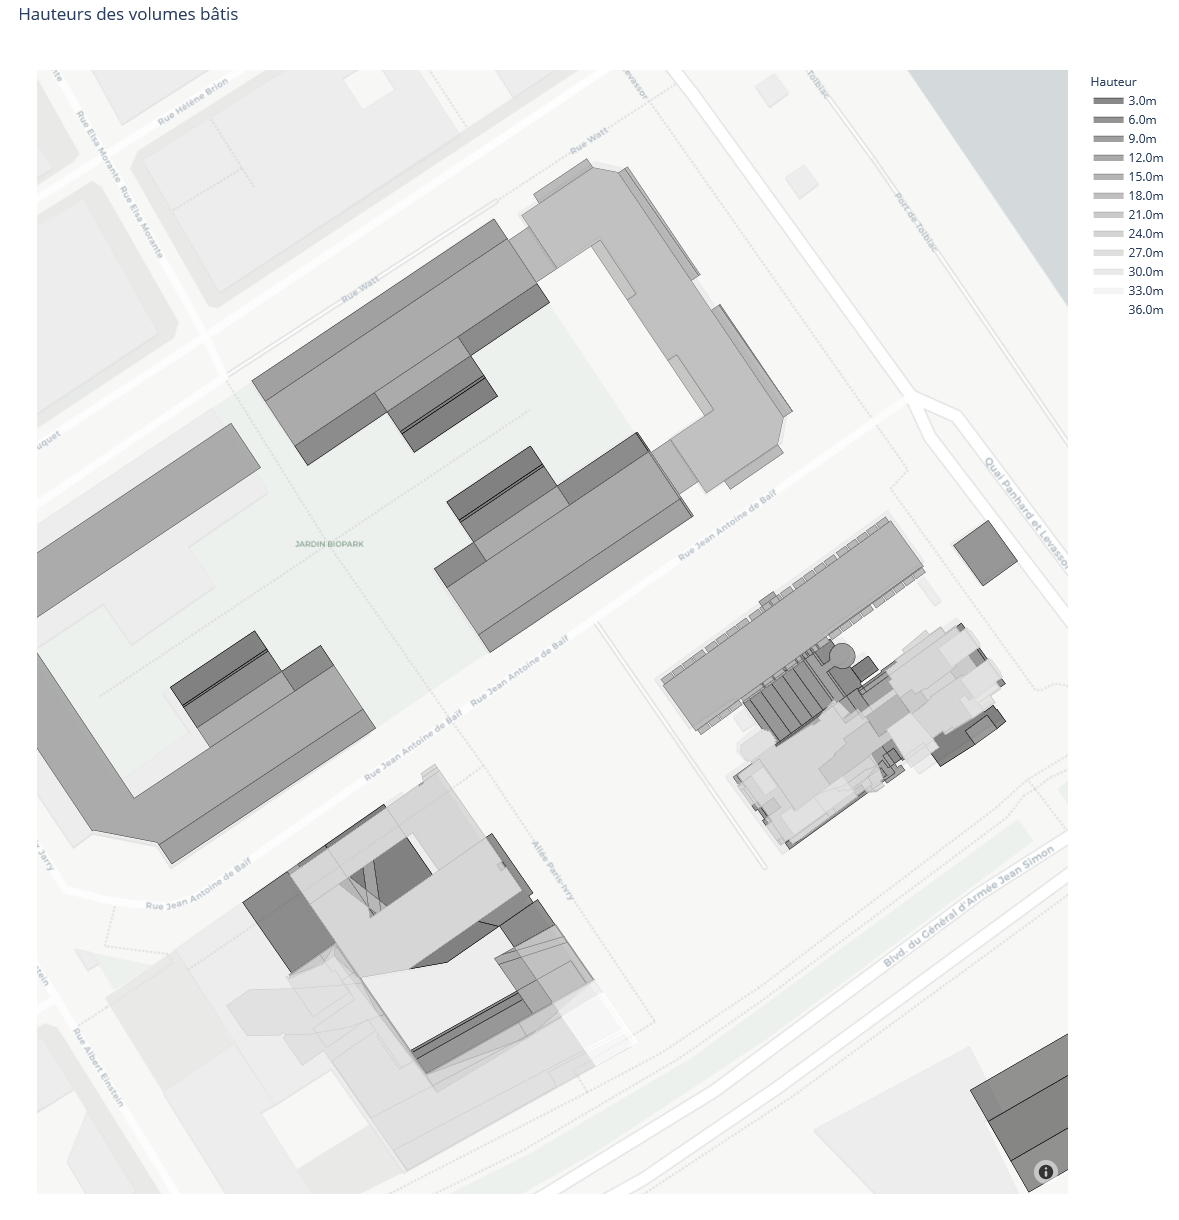
\includegraphics[width=0.45\linewidth]{__imgs/carte_hauteurs_1} 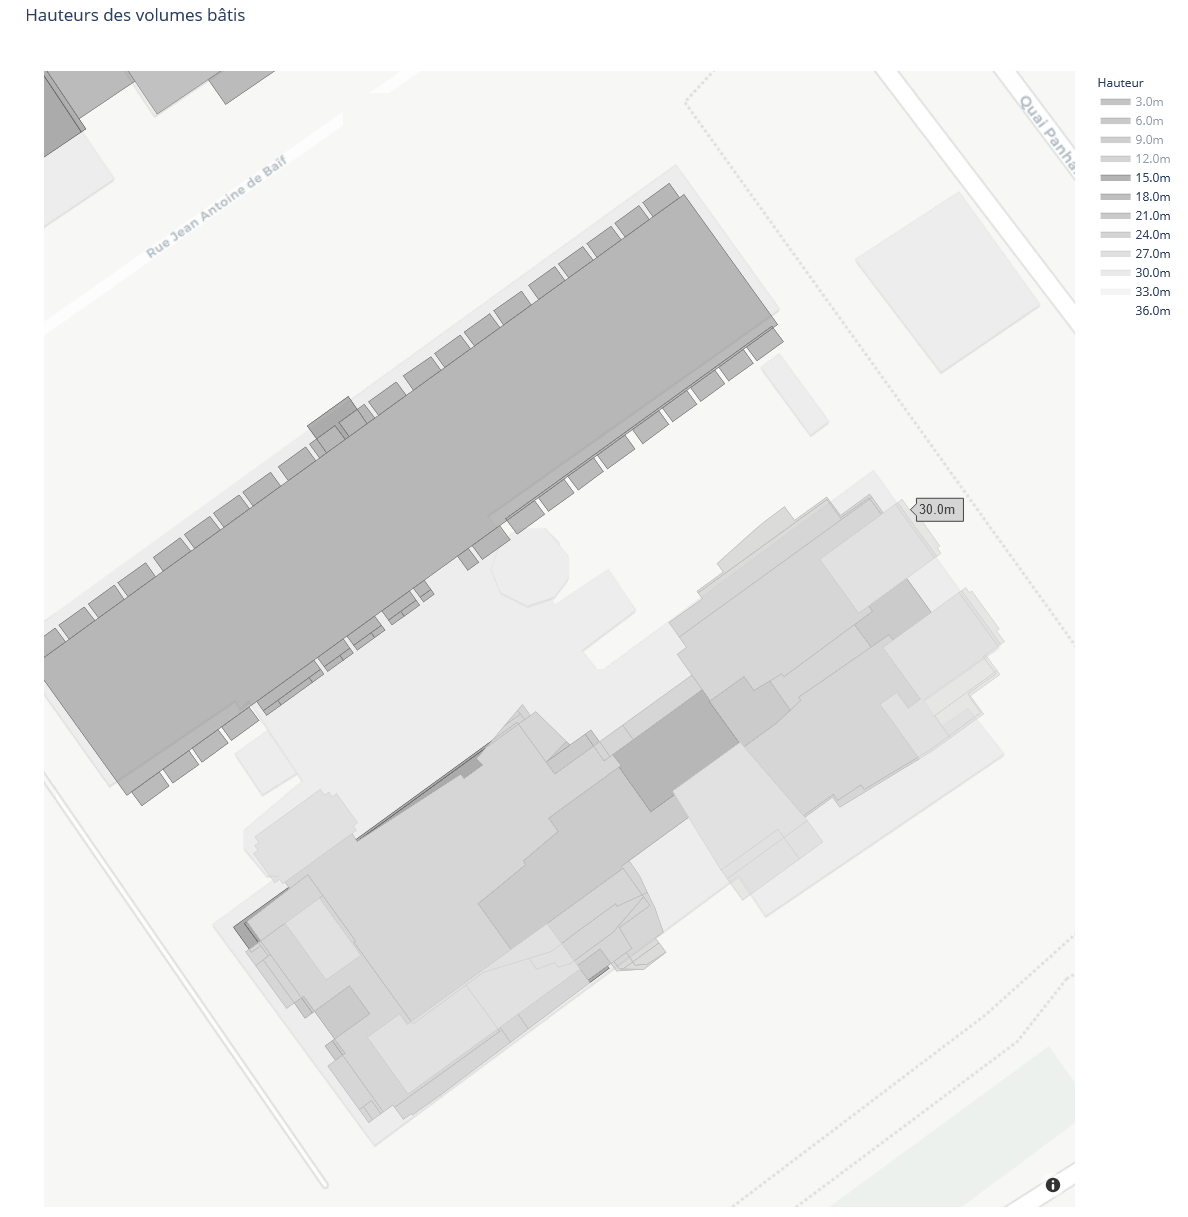
\includegraphics[width=0.45\linewidth]{__imgs/carte_hauteurs_2} 

}

\caption[Carte des volumes par hauteur avec de l'interactivité  -  Réalisation personnelle]{Carte des volumes par hauteur avec de l'interactivité}\label{fig:carte_inter}
\end{figure}
\end{tcolorbox}

Dès lors, une telle capacité à cartographier avec souplesse des données
brutes présente un intérêt certain au sein de la pratique
architecturale.

\textbf{Ainsi, ces aperçus attestent de la capacité du langage Python à
produire facilement de multiples représentations graphiques synthétiques
à partir de données brutes, du graphique statistique aux cartes
interactives, renforcant ainsi la pertinence de son utilisation dans le
cadre de l'exploitation de données issues de l'Open Data pour les
architectes.}

\newpage

\hypertarget{guxe9nuxe9ration-automatique-de-documents-techniques.}{%
\subsection{Génération automatique de documents
techniques.}\label{guxe9nuxe9ration-automatique-de-documents-techniques.}}

Les capacités de synthèse graphique et de cartographie des données
montrées précédemment sont certes intéressantes, mais le domaine de la
conception architecturale est surtout concerné par la production de
dessins, modèles 3D et autres représentations techniques à l'échelle
dans le cadre d'un projet. Cette section permettra de répondre à cet
enjeu grâce à Python.

\hypertarget{fichier-cad-vectorisuxe9-et-hiuxe9rarchisuxe9}{%
\subsubsection{Fichier CAD vectorisé et
hiérarchisé}\label{fichier-cad-vectorisuxe9-et-hiuxe9rarchisuxe9}}

Le premier aperçu livré dans cette section, sera de \textbf{produire un
document vectorisé au format .DXF} (format d'échange de dessin vectorisé
similaire au .DWG, répandu en CAO), où seront tracés les
\textbf{différents volumes sous forme de polylignes}. Chacun d'entre eux
sera également classé dans un \textbf{calque correspondant à sa
hauteur}, avec pour chaque calque une couleur différente. Pour ce faire,
le module \textbf{ezdxf} sera employé. Ce dernier permet la plupart des
fonctions de dessin vectoriel que propose d'autres outils de CAD tels
qu'\emph{AutoCAD}, dont la création de calques entre autres.\\
~\\
Cependant, il est ici indispensable de convertir les \textbf{coordonnées
géodésiques} exprimées en \emph{degrés de latitude/longitude} en
\textbf{coordonnées cartésiennes} exprimées en unités de grandeur
terrestres. Pour cela, la projection \emph{Lambert93} sera utilisée car
exprimée en \textbf{mètres} et étant \textbf{orthonormée} (son calcul
prenant en compte la rotondité de la Terre), Elle se révèle donc
essentielle pour pouvoir dessiner dans un repère tel qu'un dessin
vectorisé. Heureusement, \emph{GeoPandas} permet cette conversion, en
référençant le code du système de coordonnées de référence (crs) par
défaut (ici, le système latitude/longitude \emph{WGS84}), puis celui de
la projection \emph{Lambert93}.

\begin{tcolorbox}[title= Carte des volumes par hauteur avec de l'interactivité ,colback=boitecode]
\begin{lstlisting}[style=code]
# Coordonnées latitude/longitude (WGS84)
data.crs = 4326
# Coordonnées X/Y (Lambert93)
data = data.to_crs(2154)
# Affichage d'un exemple de coordonnées
print(data.head(1))\end{lstlisting}

```
ttvar{#}ttvar{#}                                             geometry     surface  hauteur hauteur_paf
ttvar{#}ttvar{#} 0  POLYGON ((654822.488 6858784.302, 654823.138 6...  281.214948     12.0        None
```

\end{tcolorbox}

Après l'import du module \emph{ezdxf}, un nouveau dessin est initialisé.
Ensuite, \textbf{un calque par hauteur} sera créé en amont des tracés
des volumes, de sorte à ce qu'ils apparaîssent dans un ordre croissant
au sein du futur fichier. Tout comme dans la carte interactive présentée
dans la session 2.1.2, une \textbf{teinte de couleur proportionnelle à
chaque hauteur} sera créée (en l'occurence, sur du rouge).

\begin{tcolorbox}[title= Carte des volumes par hauteur avec de l'interactivité ,colback=boitecode]
\begin{lstlisting}[style=code]
import ezdxf
# initialisation d'un nouveau dessin
doc = ezdxf.new(dxfversion='R2010')
msp = doc.modelspace()
# Récupération et tri des différentes hauteurs
hauteurs = sorted(data["hauteur"].unique())
# Itération à travers les différentes hauteurs
for h in hauteurs:
  # Création d'un nouveau calque nommé
  calque = doc.layers.new(str(h) + "m")
  # Affectation d'une couleur suivant la hauteur
  calque.rgb = (255*(h/hauteurs[-1]),0,0)\end{lstlisting}
\end{tcolorbox}

Ceci effectué, une boucle itèrera à travers chaque volume du jeu de
données (grâce à la fonction \emph{iterrows()} de \emph{GeoPandas}).
Pour chacun d'entre eux, une \textbf{polyligne} peut être tracée à
partir des coordonnées des points pour représenter l'emprise de chaque
volume, puis être affectée au calque correspondant à la hauteur du
volume.

\begin{tcolorbox}[title= Carte des volumes par hauteur avec de l'interactivité ,colback=boitecode]
\begin{lstlisting}[style=code]
for row,volume in data.iterrows():
    # Extraction des coordonnées des points du polygone
    coords = list(zip(*volume["geometry"].exterior.coords.xy))
    # Affectation au sein du calque correspondant à sa hauteur
    calque = str(volume["hauteur"]) + "m"
    msp.add_polyline2d(coords, dxfattribs={'layer': calque})\end{lstlisting}
\begin{lstlisting}[style=code]
doc.saveas("OUTPUT/plan_bati.dxf")\end{lstlisting}
\end{tcolorbox}

\begin{tcolorbox}
\begin{figure}

{\centering 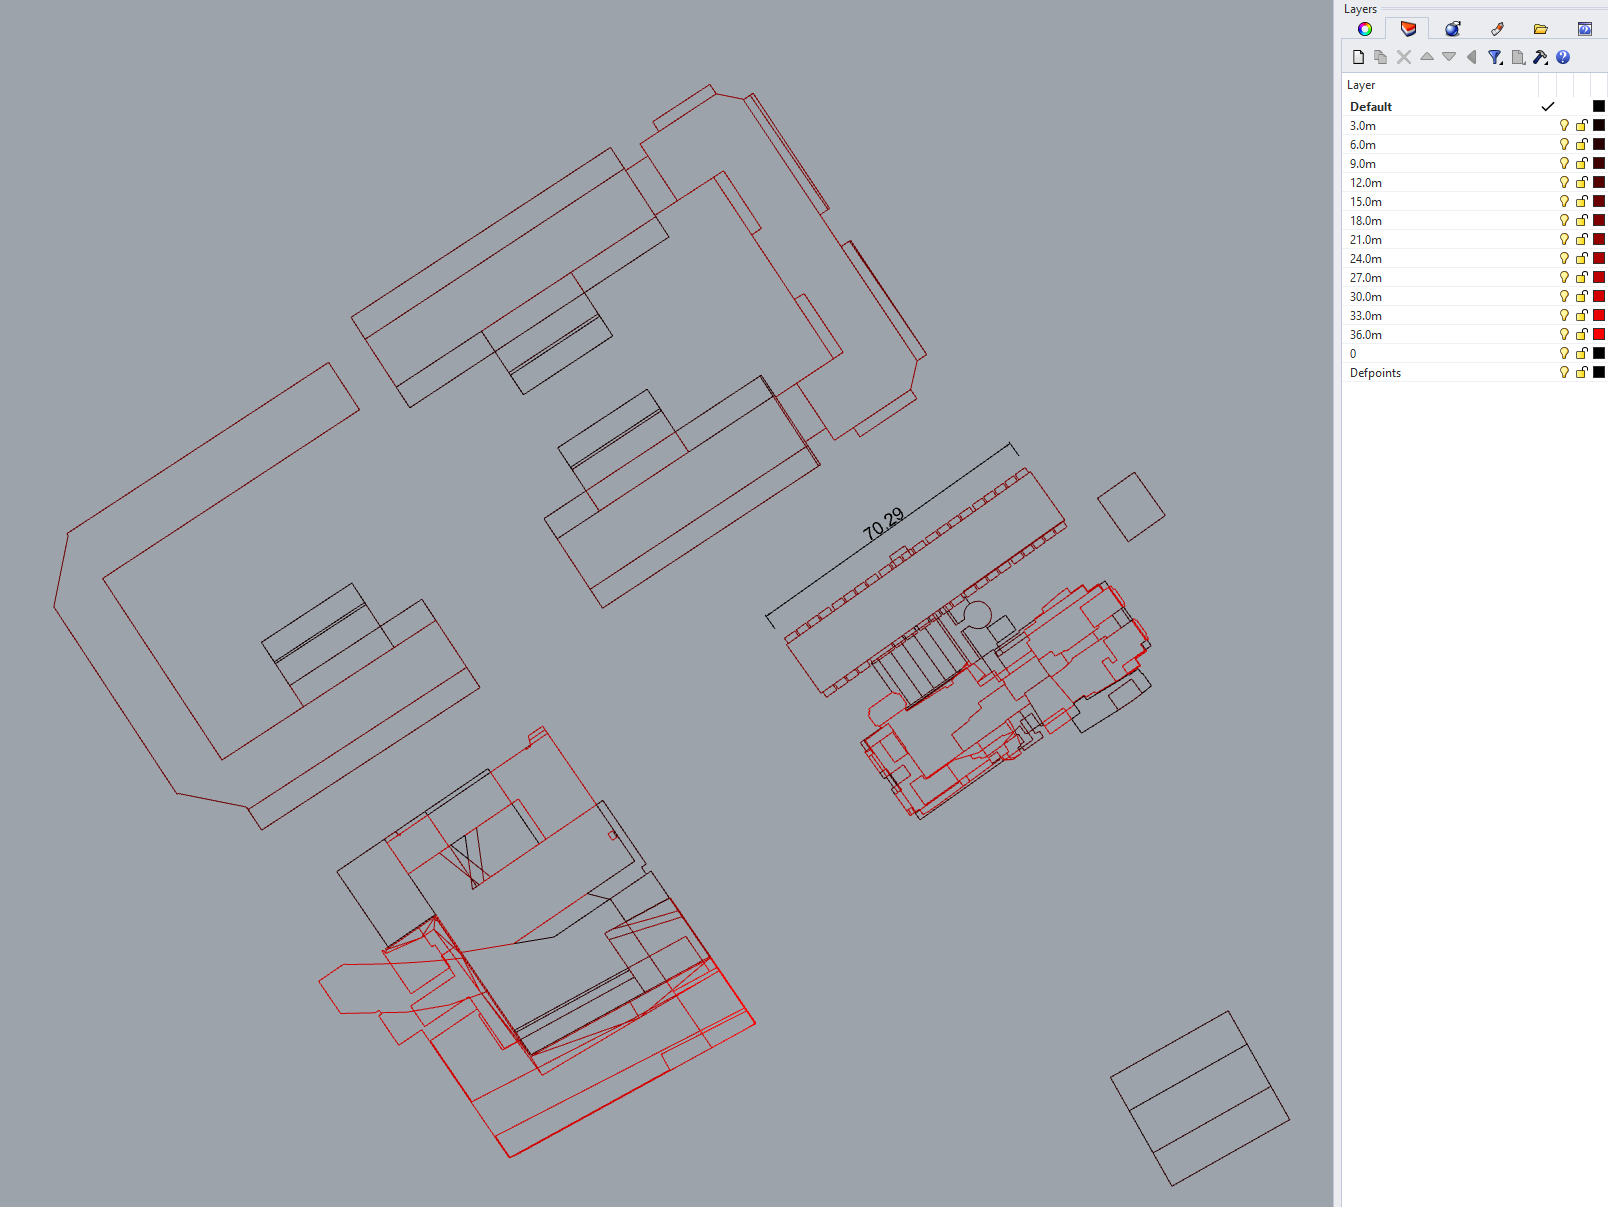
\includegraphics[width=0.9\linewidth]{__imgs/cad_1} 

}

\caption[Fichier vectoriel organisé des emprises des volumes  -  Réalisation personnelle]{Fichier vectoriel organisé des emprises des volumes}\label{fig:dessin_cad}
\end{figure}
\end{tcolorbox}

Le document fourni en sortie peut ensuite être importé dans n'importe
quel logiciel supportant le format DXF, ce qui est le cas pour la
majorité des outils de dessin vectoriel des agences d'architecture. Ce
document est d'autant plus exploitable qu'il reste \textbf{géoréférencé}
(les volumes conservent leurs coordonnées \emph{Lambert93} dans le
dessin), et \textbf{à l'échelle} (puisque ces coordonnées sont exprimés
en mètres).\\
De plus, les options de \textbf{personnalisation} des calques permettent
de hiérarchiser les données dont on dispose en amont d'une exploitation
``manuelle''.

Ainsi, le langage Python prouve également son efficacité lorsqu'il est
question de générer des documents vectoriels graphiques, pleinement
exploitables comme support de travail.

\hypertarget{construction-dun-moduxe8le-3d}{%
\subsubsection{Construction d'un modèle
3D}\label{construction-dun-moduxe8le-3d}}

Cette sous-section aura pour but de clore le chapitre en exploitant à
son plein potentiel le jeu de donné extrait. En effet, puisque l'on
dispose à la fois d'\textbf{emprises géométriques traçables} ainsi que
de \textbf{hauteurs}, construire un \textbf{modèle 3D} automatiquement
se présente comme un aboutissement certain, d'autant plus qu'il
représente tout naturellement une forte utilité pour l'architecte.\\
~\\
Bien que Python possède des bibliothèques permettant de manipuler de la
3D telles que \textbf{PyOpenGL}\footnote{\emph{PyOpenGL -- The Python
  OpenGL Binding} {[}en~ligne{]}. 24 janvier 2021. Disponible à
  l'adresse\,: \url{http://pyopengl.sourceforge.net/}.} ou
\textbf{Open3D},\footnote{ZHOU, Qian-Yi, PARK, Jaesik et KOLTUN,
  Vladlen. {Open3D}: {A} Modern Library for {3D} Data Processing.
  \emph{arXiv:1801.09847}. 2018.} ces dernières sont plutôt orientées
pour effectuer des rendu en images de synthèses ou de la reconstruction
sur des maillages. Or, ces fonctionnalités sont assez éloignées de
l'usage souhaité, où l'on cherche plutôt à \textbf{construire un modèle
3D} à partir de données brutes puis les exporter dans des formats
possédant des \textbf{capacités d'organisation du modèle} (comme des
calques par exemple) et en évitant le \textbf{maillage}, afin de les
rendre compatibles avec l'usage qu'en feraient un architecte. Ce n'est
pas le cas ici, les bibliothèques citées privilégiant les formats
d'échange maillés comme le format OBJ.\\
De plus, même si ce retard a tendance à diminuer avec leur évolution, la
quasi-totalité des bibliothèques orientées 3D pour Python sont basées
sur des versions codées dans des langages de programmation plus
complexes comme le \emph{C++} pour des raisons de performances, ce qui
fait qu'il persiste toujours un ``retard'' entre le moteur natif et son
intégration destinée à Python, comme le présente plus en détail
l'ouvrage \emph{Python \& OpenGL for Scientific Visualization}
(P.ROUGIER,2018).\footnote{P.ROUGIER, Nicolas. \emph{Python \& OpenGL
  for Scientific Visualization}. Bordeaux\,: {[}s.~n.{]}, 2018.
  Disponible à l'adresse\,:
  \url{https://www.labri.fr/perso/nrougier/python-opengl/}.}\\
C'est pourquoi la bibliothèque \textbf{RhinoInside}\footnote{\emph{Rhino
  - Rhino.Inside} {[}en~ligne{]}. 25 janvier 2021. Disponible à
  l'adresse\,: \url{https://www.rhino3d.com/features/rhino-inside/}.}
sera ici utilisée. C'est un outil Open Source développé sous
l'initiative de la société Mcneel, intégré au logiciel de modélisation
3D \textbf{Rhinoceros} depuis la version 7. Il a en effet pour but de
\textbf{connecter Rhinoceros à un autre programme éxecuté en parallèle},
afin de mettre en place un moyen d'échange direct de données.\\
La version Python de cette bibliothèque permet en l'occurrence de
connecter une instance de Rhinoceros sans interface graphique à un
script (mais permettant tout de même toute opération possible
manuellement dans le logiciel). Autrement dit, il sera possible
directement dans un même script de créer un fichier au format natif de
Rhinoceros (.3DM), puis y dessiner et extruder des tracés pour enfin le
sauvegarder sur son disque dur.\\

\begin{tcolorbox}[title= Fichier vectoriel organisé des emprises des volumes ,colback=boitecode]
\begin{lstlisting}[style=code]
import rhinoinside
from pathlib import Path
rhino_path = Path("C:/Program Files/Rhino 7/System")
rhinocore_path = Path("C:/Program Files/Rhino 7/System/RhinoCore.dll")
rhinoinside.load(str(rhino_path))
import System
import Rhino\end{lstlisting}
\end{tcolorbox}

La séquence d'import ci-dessus est plus conséquente, puisqu'il faut ici
spécifier le chemin d'installation de Rhino 7.

\begin{tcolorbox}[title= Fichier vectoriel organisé des emprises des volumes ,colback=boitecode]
\begin{lstlisting}[style=code]
# Création du document
DOC = Rhino.RhinoDoc.Create("")
DOC.ModelUnitSystem = Rhino.UnitSystem.Meters
# Création d'un calque principal
calque_bati =  Rhino.DocObjects.Layer()
calque_bati.Color = System.Drawing.Color.FromArgb(255,0,0,0)
calque_bati.Name = 'batiments'
DOC.Layers.Add(calque_bati)
# Définition de ce calque comme actuel\end{lstlisting}
\begin{lstlisting}[style=code]
c_actuel = DOC.Layers.FindByFullPath("calque_bati",-1)
DOC.Layers.SetCurrentLayerIndex(c_actuel,False)\end{lstlisting}
\end{tcolorbox}

Une première étape consiste à créer un \textbf{nouveau document rhino},
spécifier ses unités (ici, en accord avec les unités des coordonnées
\emph{Lambert93}, soit le \emph{mètre}), ainsi que créer un calque dans
lequel seront dessinés les volumes. Ce dernier se verra attribuer un
\textbf{nom} et une \textbf{couleur}.

\begin{tcolorbox}[title= Fichier vectoriel organisé des emprises des volumes ,colback=boitecode]
\begin{lstlisting}[style=code]
for row,volume in data.iterrows():
  # Liste de points vide pour créer une polyligne
  pts = System.Collections.Generic.List[Rhino.Geometry.Point3d]()
  # Extraction des coordonnées des points du polygone
  coords = list(zip(*volume["geometry"].exterior.coords.xy))
  for c in coords:
    # Ajout des points du polygone
    pts.Add(Rhino.Geometry.Point3d(c[0],c[1],0.0))
  # Création de la polyligne
  poly = Rhino.Geometry.Polyline(pts)
  if volume["hauteur_paf"] == None:
    # Si le volume repose au rdc
    polyz = poly.ToPolylineCurve()
    # Création de l'extrusion
    extr = Rhino.Geometry.Extrusion.Create(polyz,-1*float(volume["hauteur"]),True)
    DOC.Objects.AddExtrusion(extr)
  else:
    # Si le volume est en porte à faux
    # Itération à travers les intervalles
    for intervalle in volume['hauteur_paf']:
      poly.SetAllZ(float(intervalle[0]))
      polyz = poly.ToPolylineCurve()
      h_cible = float(intervalle[1])-float(intervalle[0])
      # Création de l'extrusion entre les limites de l'intervalle
      extr = Rhino.Geometry.Extrusion.Create(polyz,-1*h_cible,True)
      DOC.Objects.AddExtrusion(extr)
  \end{lstlisting}
\begin{lstlisting}[style=code]
success = DOC.SaveAs('OUTPUT/modele.3dm')\end{lstlisting}
\end{tcolorbox}

La boucle ci-dessus effectue deux opérations distinctes sur chaque
volume.\\
La première étape consiste à \textbf{extraire les points de chaque
polygone} et de les grouper au sein d'une liste (nommée \emph{pts}) afin
d'en générer une \textbf{polyligne}.\\
Ensuite, si le volume repose simplement en rez-de-chaussée, une seule
extrusion sera créée afin d'atteindre la hauteur définie par l'attribut
\emph{hauteur}, puis sera écrite dans le fichier. En revanche, si le
volume est en \textbf{porte à faux}, les différents \textbf{intervalles
de hauteur} qu'il occupe dans son emprise en plan (exemple : 6 à 15
mètres) sont traités à travers une boucle. Pour chacun d'entre eux, la
polyligne créée précédemment sera déplacée en hauteur pour atteindre la
borne ``basse'' de l'intervalle. Une \textbf{extrusion} est alors créée
depuis cette base pour atteindre la hauteur définie par la borne
``haute'' de l'intervalle, et sera enfin écrite dans le fichier
Rhinoceros.\\
~\\
Enfin, le fichier est sauvegardé au format 3DM, que l'on peut ensuite
visualiser et parcourir directement dans Rhinoceros.

\begin{tcolorbox}
\begin{figure}

{\centering 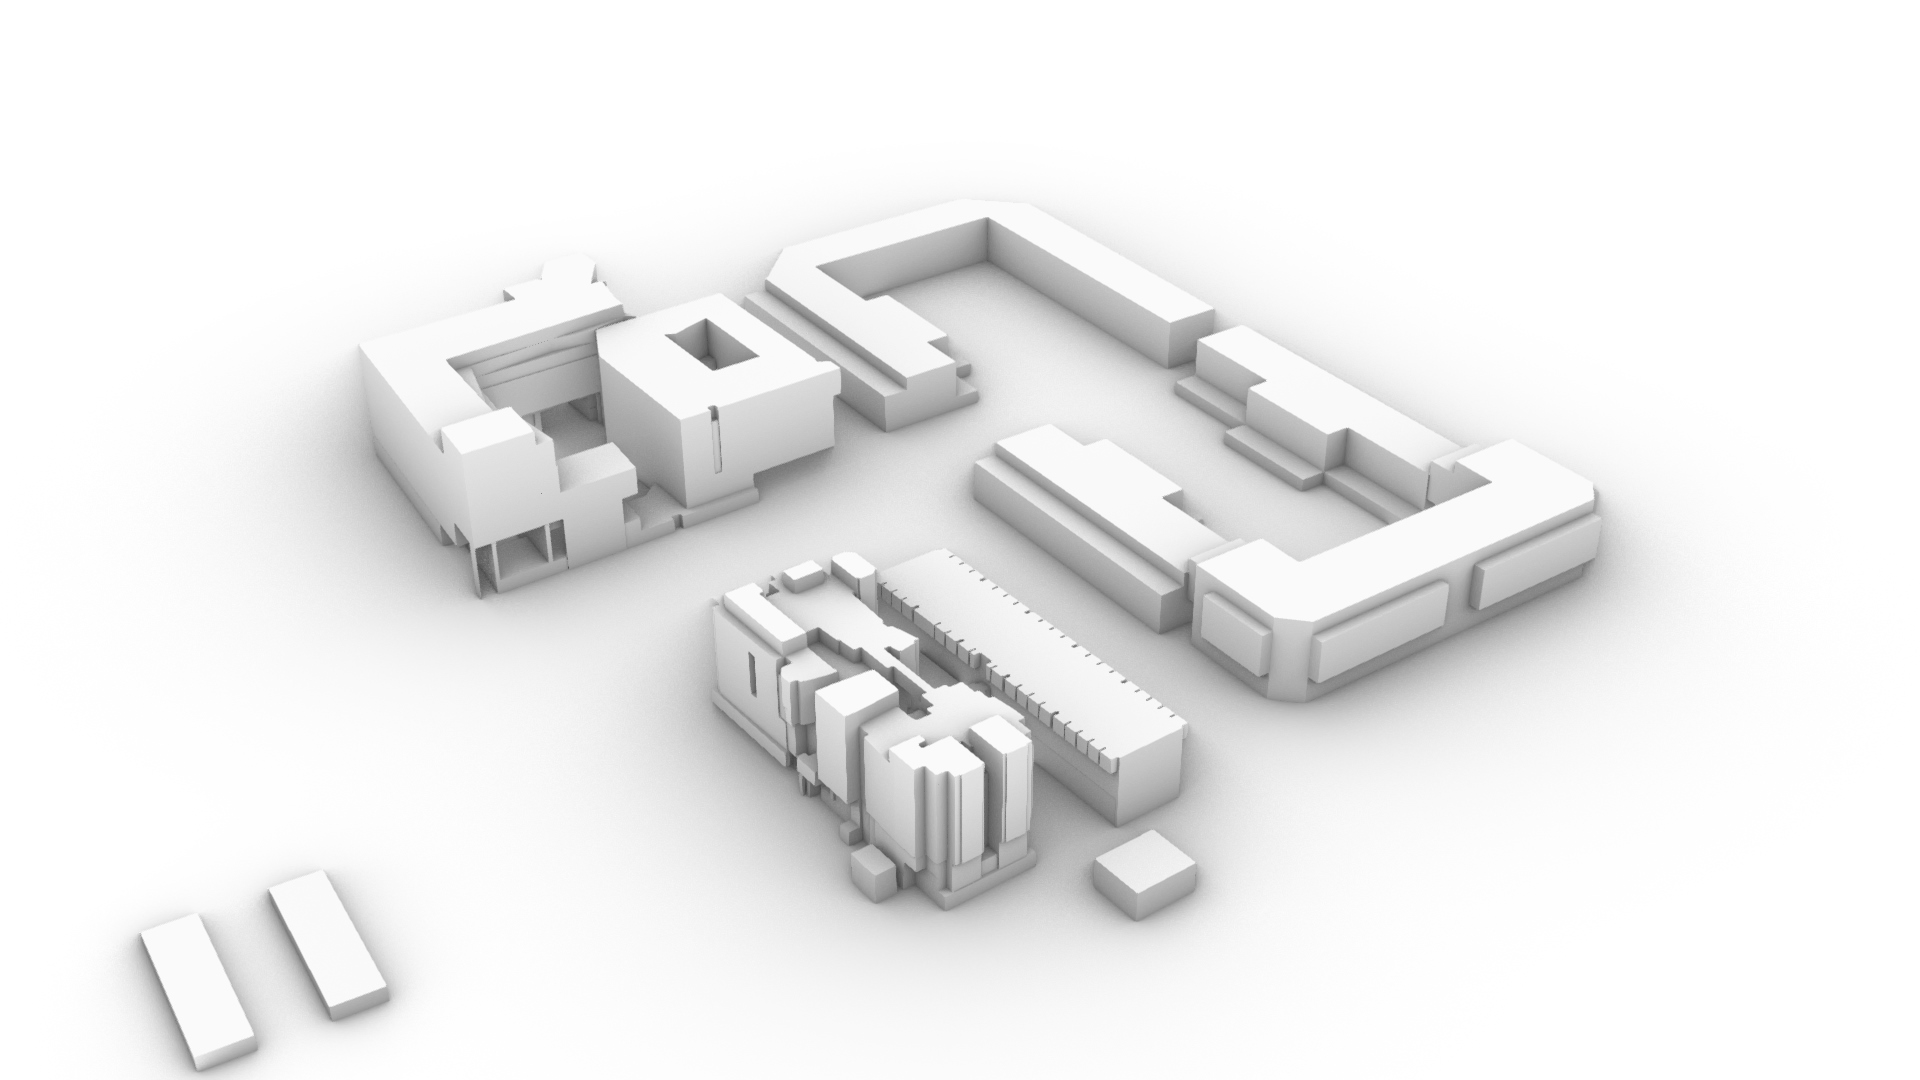
\includegraphics[width=0.9\linewidth]{__imgs/3d_vue1} 

}

\caption[Modèle 3D généré grâce aux données de hauteur des volumes  -  Réalisation personnelle]{Modèle 3D généré grâce aux données de hauteur des volumes}\label{fig:modele_3d}
\end{figure}
\end{tcolorbox}

Le résultat révèle à la fois une \textbf{précision} et un \textbf{degré
de complexité} certains du jeu de données initial, jusque-là
non-visualisables.

\begin{tcolorbox}
\begin{figure}

{\centering 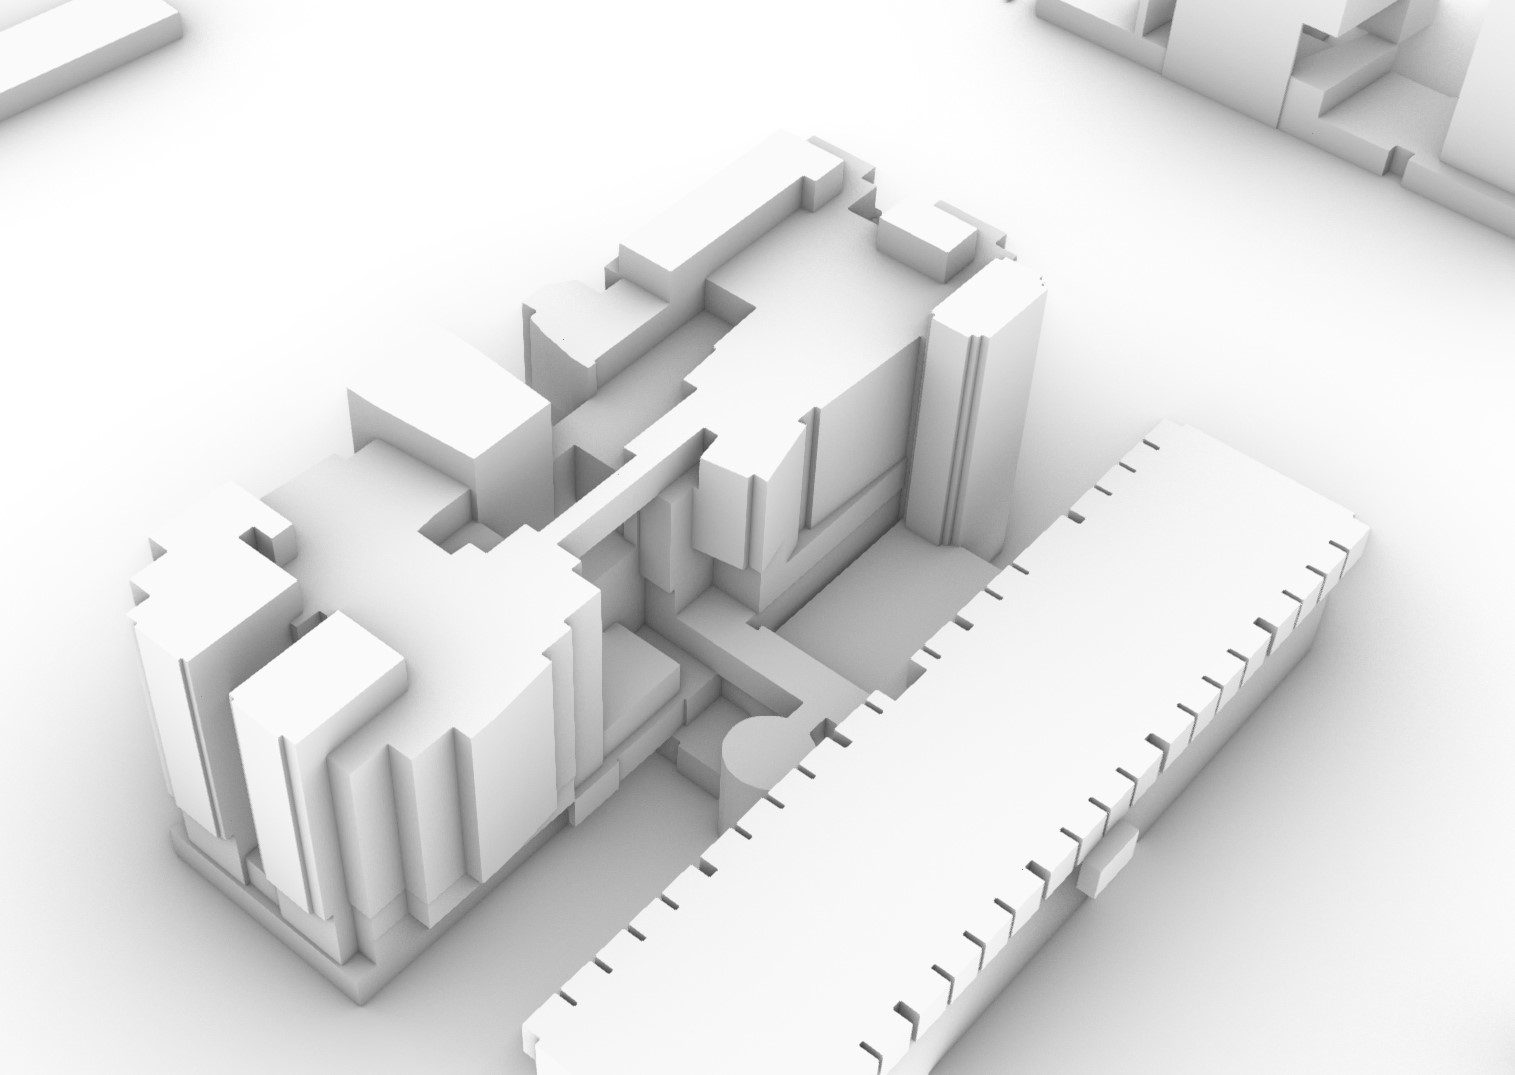
\includegraphics[height=0.3\textheight]{__imgs/3d_zoom_1} 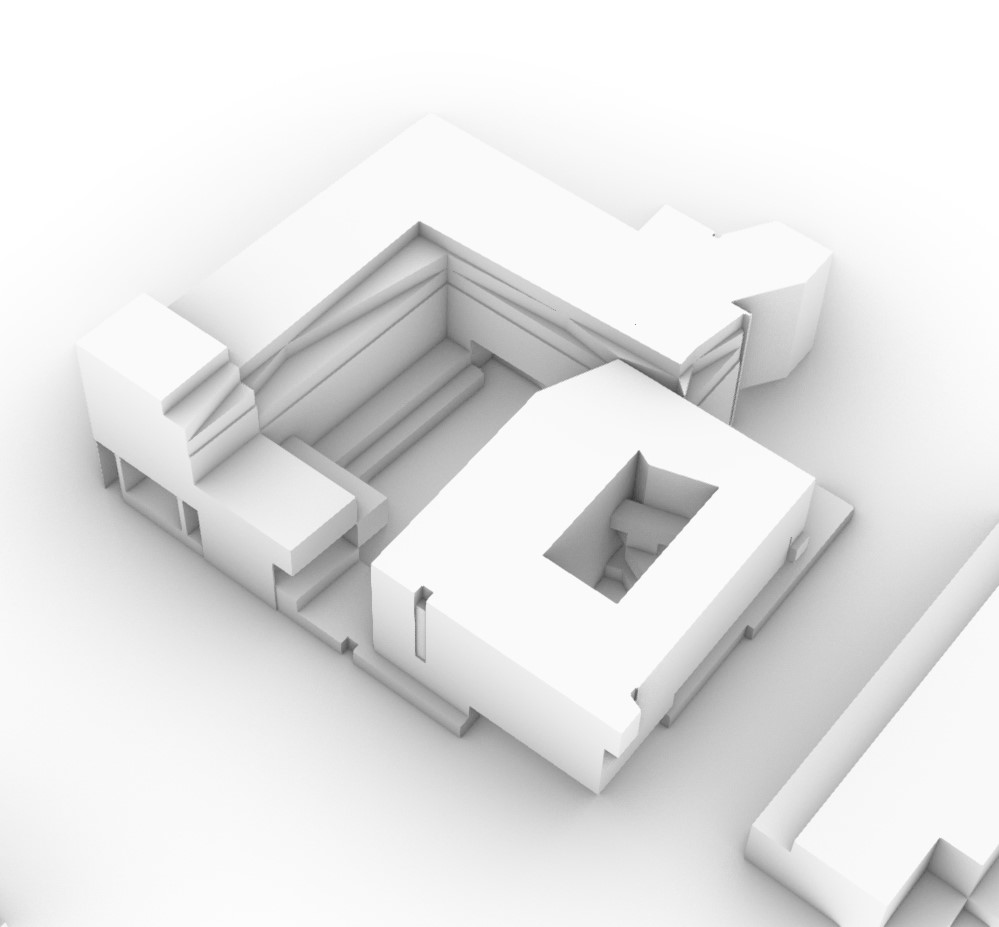
\includegraphics[height=0.3\textheight]{__imgs/3d_zoom_2} 

}

\caption[Une précision et une richesse rendue visible grâce à la modélisation  -  Réalisation personnelle]{Une précision et une richesse rendue visible grâce à la modélisation}\label{fig:modele_3d_zoom}
\end{figure}
\end{tcolorbox}

Bien que la syntaxe de \textbf{Rhinoinside} soit plus ardue que celle de
la section précédente (dû au fait qu'il est nécessaire de s'appuyer sur
de la documentation écrite pour le langage de programmation natif de
Rhinoceros, le \emph{C\#}), un architecte possédant une bonne
connaissance du logiciel Rhinoceros, et surtout de la manière logique de
résoudre un problème de modélisation dans cet outil précis (surtout vis
à vis des commandes) peut établir une stratégie viable.\\
\textbf{Cette solution a donc permis d'exploiter les données collectées
à leur plein potentiel.}\\
~\\
\textbf{Ainsi, au-delà de permettre une simple visualisation statistique
des jeux de données en Open Data, le langage Python apporte à
l'architecte des solutions techniques variées afin de convertir les jeux
de données bruts en fichiers synthétiques dans des formats pleinements
exploitables dans son environnement de travail, de la visualisation des
données interactives au modèle 3D.}\\
~\\
En outre, tous les scripts présentés permettent d'obtenir chacun de ces
éléments en \textbf{un temps d'éxécution très faible (quelques minutes
tout au plus)}, permettant un \textbf{gain de temps considérable} une
fois qu'ils ont été développés, qui ne fera que \textbf{s'accroître} à
mesure qu'on les \textbf{réutilise}. De plus, ils démontrent par leur
\textbf{longueur maîtrisée} (50 lignes maximum) que ce genre de
manipulations complexes peuvent être mises en place de manière clarifiée
(grâces aux bibliothèques comme \emph{GeoPandas}), en prolongement des
concepts abordés dans le chapitre 1.\\
~\\
Jusqu'à lors, l'exercice a été de manipuler une infime portion d'un jeu
de données ciblé autour d'un site, dans une optique « traditionnelle »
de se renseigner sur un contexte immédiat. Le prochain chapitre sera
dédié à une approche plus approfondie de l'utilisation de données
ouvertes, recélant cependant un intérêt certain pour la conception
architecturale.

\newpage

\hypertarget{exploiter-lopen-data-pour-entrauxeener-des-moduxe8les-de-pruxe9diction}{%
\section{Exploiter l'Open Data pour entraîner des modèles de
prédiction}\label{exploiter-lopen-data-pour-entrauxeener-des-moduxe8les-de-pruxe9diction}}

A l'instar du jeu de données étudié au cours des chapitres précédents
dont un échantillon spécifique a été prélevé, la \textbf{massivité d'un
jeu de données} est une caractéristique courante en Open Data. Dès lors,
au vu de leur grande taille, certains jeux peuvent être considérés comme
suffisamment \textbf{représentatifs} vis à vis de ce qu'ils recensent.
Autrement dit, c'est une véritable source de connaissances numérique.\\
~\\
Or, le domaine de \textbf{l'Intelligence Artificielle}, et tout
particulièrement le \textbf{Machine Learning} se reposent sur des
données disponibles en grande quantité pour pouvoir entraîner des
algorithmes. En effet, la précision d'un algorithme étant lié à sa
capacité à \textbf{généraliser} les connaissances qu'on lui fournit lors
d'une session d'entraînement, il convient de disposer de données
suffisamment \textbf{variées et exhaustives}, tout en étant \textbf{en
grand nombre} afin de permettre un apprentissage optimal.\\
~\\
Il s'avère également que le langage de programmation Python figure parmi
les langages les mieux équipés pour le Machine Learning, disposant de
bibliothèques comme \textbf{Scikit-Learn}\footnote{\emph{Scikit-learn:
  machine learning in Python} {[}en~ligne{]}. {[}s.~d.{]}.
  {[}Consulté~le~16~janvier~2021{]}. Disponible à l'adresse\,:
  \url{https://scikit-learn.org/stable/}.} proposant une approche
simplifiée à travers des algorithmes primaires, jusqu'aux plateformes
majeures du secteur comme \textbf{TensorFlow}\footnote{\emph{TensorFlow}
  {[}en~ligne{]}. {[}s.~d.{]}. {[}Consulté~le~20~janvier~2021{]}.
  Disponible à l'adresse\,: \url{https://www.tensorflow.org/}.} ou
\textbf{PyTorch}\footnote{\emph{PyTorch} {[}en~ligne{]}. {[}s.~d.{]}.
  {[}Consulté~le~20~janvier~2021{]}. Disponible à l'adresse\,:
  \url{https://pytorch.org/}.} majoritairement basées sur ce langage
proposant des fonctionnalités plus approfondies.\\
~\\
\textbf{Un enjeu de taille apparaît alors, celui d'être en capacité
d'entraîner un modèle de prédiction exploitable dans la pratique
professionnelle de l'architecte basé sur des donnéees accessibles en
Open Data}\\
~\\
Ce chapitre sera justement centré sur un algorithme que j'ai développé
au cours du Semestre 9 dans le cadre de mon Projet de Fin d'Études,
\textbf{capable d'approcher quantitativement des gisements de matériaux
sur l'existant}, en particulier sur la phase initiale concernant
\textbf{l'état des lieux des données} ainsi que leur
\textbf{exploitation avec le langage Python} .

\newpage

\hypertarget{probluxe9matique-du-moduxe8le-de-pruxe9diction}{%
\subsection{Problématique du modèle de
prédiction}\label{probluxe9matique-du-moduxe8le-de-pruxe9diction}}

Le développement de cet outil ayant émergé selon un besoin précis dans
le cadre d'une intervention architecturale, cette première section aura
pour but de présenter le cadre de la démarche ainsi que les données
mobilisées.

\hypertarget{du-contexte-uxe0-la-duxe9marche}{%
\subsubsection{Du contexte à la
démarche}\label{du-contexte-uxe0-la-duxe9marche}}

La volonté de mettre en place un algorithme prend ses racines sur une
problématique contextuelle liée au site d'intervention ciblé.\\
Le site en question est celui des anciens entrepôts du BHV (Bazar de
l'Hotel de Ville) à Ivry sur Seine. Cet immense terrain laissé à l'état
de friche depuis 2013 est situé au sein de la \textbf{ZAC
Ivry-Confluences}, ancien territoire fortement industrialisé \textbf{en
renconversion} depuis une dizaine d'années.\\
~\\

\begin{tcolorbox}
\begin{figure}

{\centering 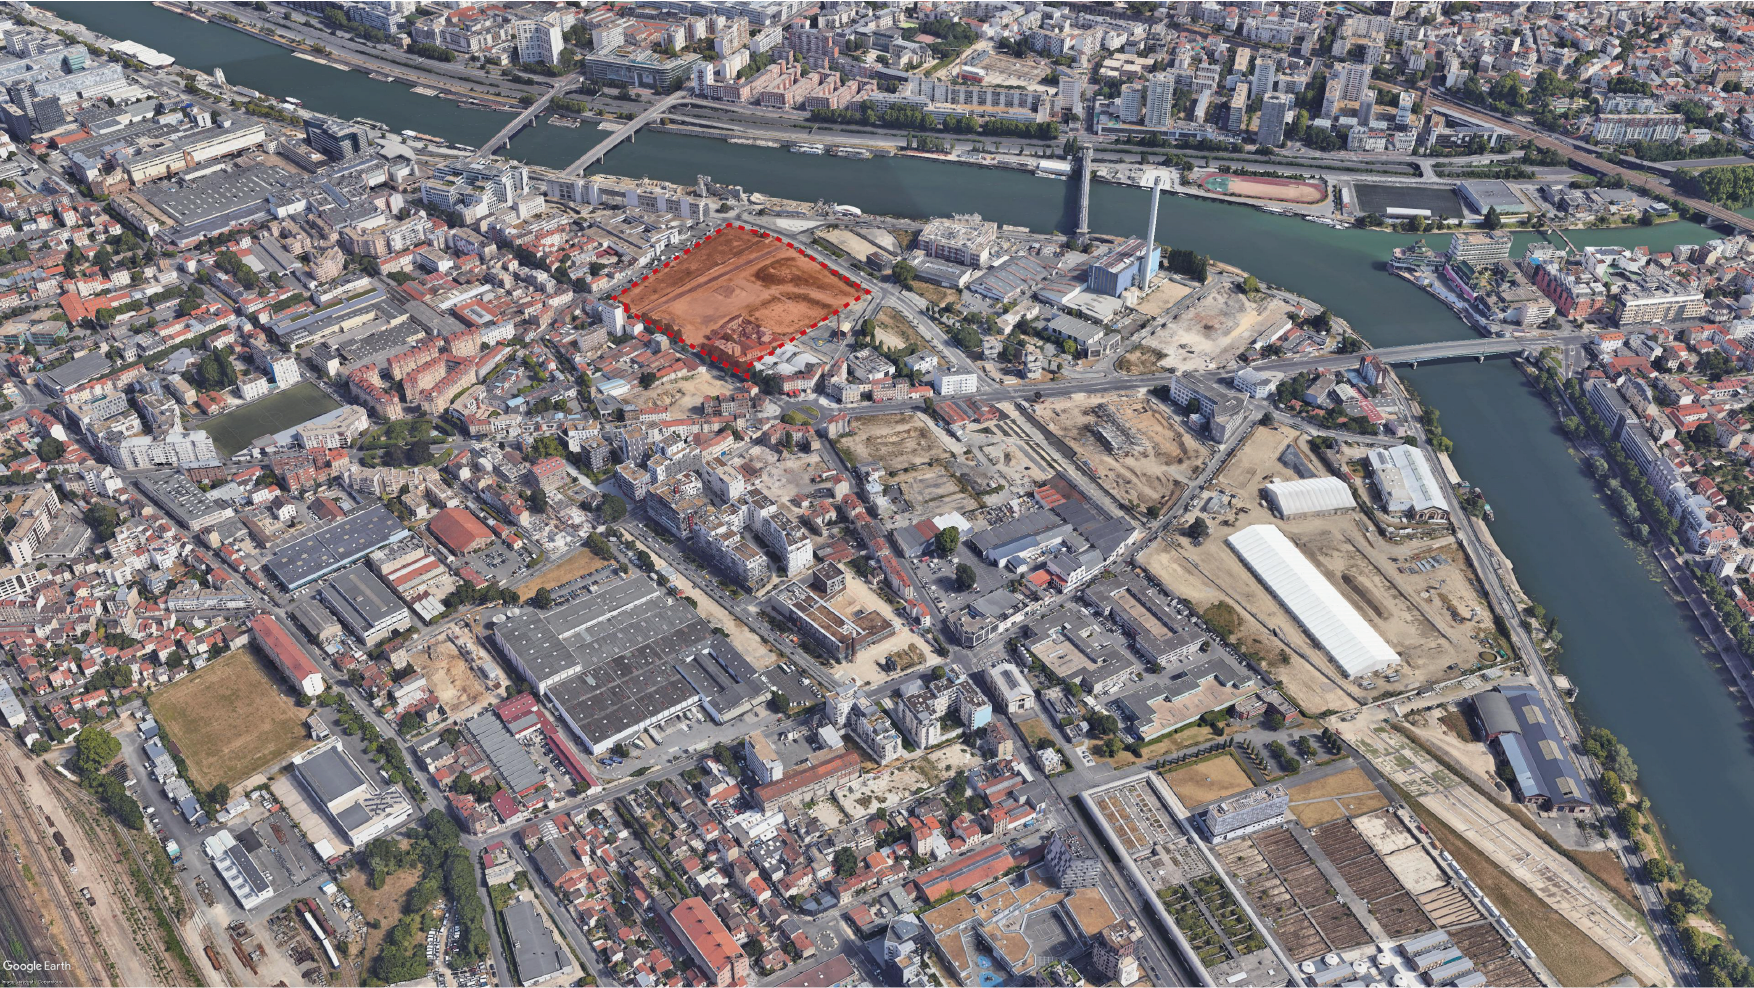
\includegraphics[width=0.9\linewidth]{__imgs/zac_photo} 

}

\caption[Photographie aérienne de la ZAC Ivry Confluences, contexte du site choisi  -  Google Earth]{Photographie aérienne de la ZAC Ivry Confluences, contexte du site choisi}\label{fig:zac_photo}
\end{figure}
\end{tcolorbox}

\hfill\break
\hfill\break
Bien que cette reconversion aie pour volonté de conserver un maximum de
bâti industriel existant, elle sera malgré tout à l'origine de
nombreuses \textbf{démolitions}, notamment à cause de la vétusté d'une
partie de ce patrimoine et le nouveau tissu urbain induisant une
multitude de nouvelles voies de circulation découpant les grands îlots
existants.\\
~\\

\begin{tcolorbox}
\begin{figure}

{\centering 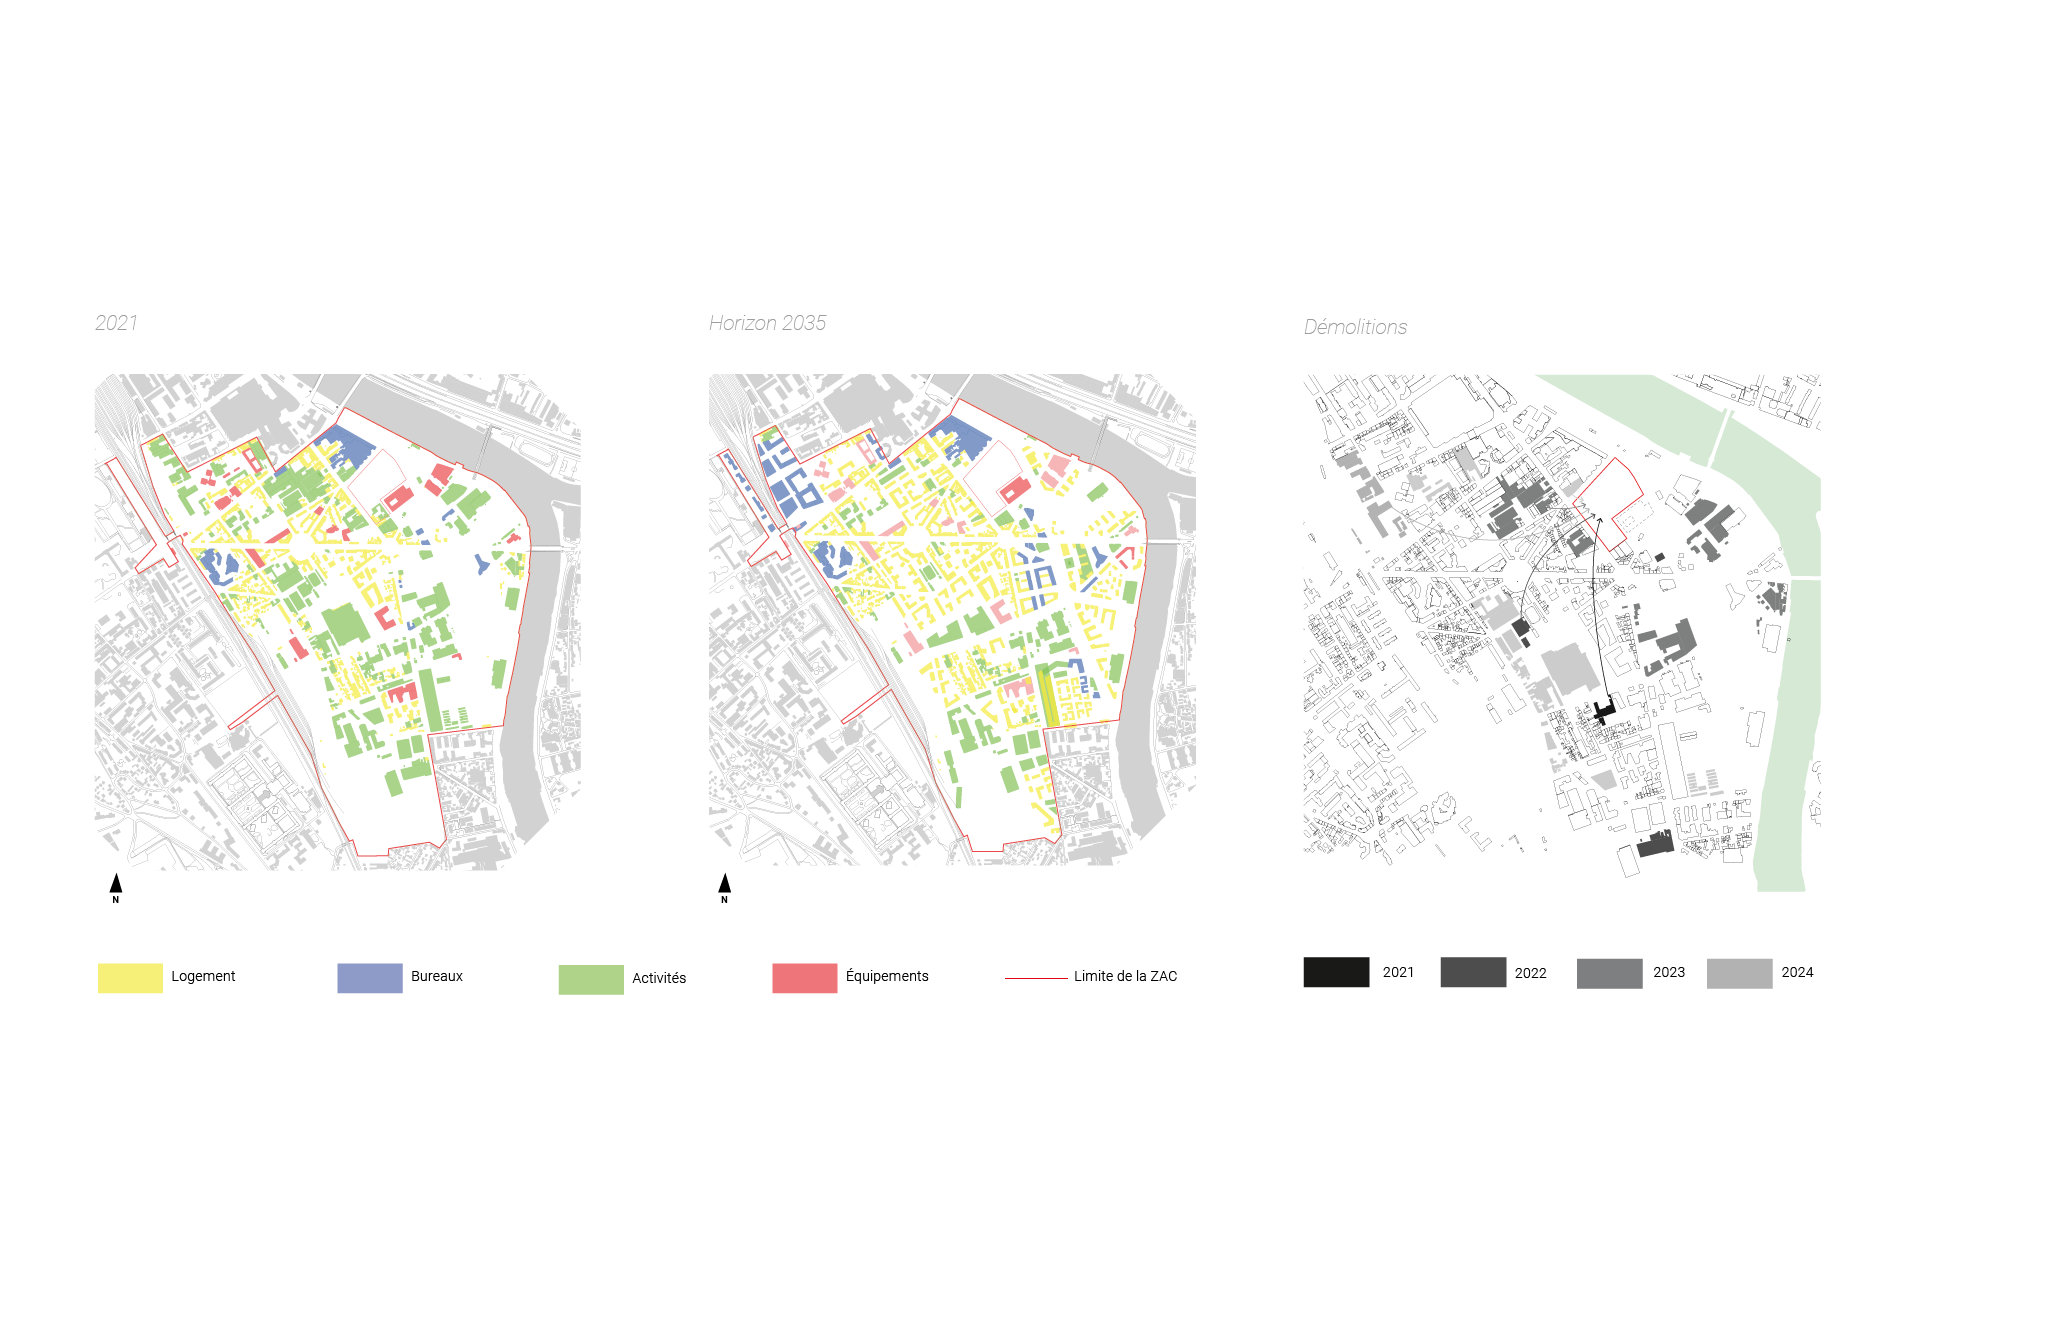
\includegraphics[width=0.9\linewidth]{__imgs/zac_schema} 

}

\caption[Transformation de la ZAC et temporalitée des démolitions  -  Réalisation personnelle]{Transformation de la ZAC et temporalitée des démolitions}\label{fig:zac_schema}
\end{figure}
\end{tcolorbox}

\hfill\break
\hfill\break
Dès lors, il existe un véritable enjeu autour de la
\textbf{valorisation} de ces gisements de métariaux de réemploi issus de
la démolition, dont j'ai alors immédiatement envisagé de me saisir comme
ressources de construction. Inévitablement, il est nécessaire de les
approcher à la fois de manière \textbf{qualitative et quantitative} afin
de pouvoir les exploiter pleinement au sein d'un projet.

\hypertarget{approche-des-objectifs-du-moduxe8le}{%
\subsubsection{Approche des objectifs du
modèle}\label{approche-des-objectifs-du-moduxe8le}}

Après avoir identifié la \textbf{chronologie la plus cohérente} des
bâtiments à démolir grâce aux documents rendus disponible par les
collectivités locales, il restait alors deux obstacles de taille :\\
* A cause de la quantité importante de bâtiments identifiés, ainsi que
l'inaccessibilité de la plupart de ces gisements, l'approche
\textbf{qualitative} paraît alors complexe à mettre en oeuvre.

\begin{itemize}
\tightlist
\item
  Bien que l'on puisse disposer d'\textbf{informations morphologiques
  basiques} concernant les bâtiments existants (en partie grâce au
  cadastre vectorisé), il est impossible d'en extraire de quelconques
  mesures plus précises essentielles à une estimation
  \textbf{quantitative} de matériaux à récupérer, telles que la
  \textbf{surface vitrée} ou encore l'\textbf{épaisseur de façade}.\\
  ~\\
  Ainsi, un \textbf{algorithme de prédiction} capable de
  \textbf{d'approcher le principal potentiel de matériaux à réemployer}
  d'un bâtiment grâce à une \textbf{approximation de leur nature et leur
  quantité} se révèlerait ici particulièrement utile, entraîné à partir
  d'un jeu de données sur des bâtiments existants dans un contexte
  géographique proche (la région Ile de France par exemple).\\
  ~\\
  Enfin, quant aux données à fournir en entrée de l'algorithme
  concernant le bâti à démolir, le point de départ sera la
  \textbf{morphologie}. Toute information complémentaire susceptible
  d'être utile lors de la prédiction (c'est à dire liée directement ou
  indirectement à la nature ou la quantité de métariaux à réemployer)
  doit être \textbf{facilement obtenable} à cette échelle (idéalement
  grâce à un jeu de données capable d'être intégré à la représentation
  3D).
\end{itemize}

\newpage

\hypertarget{lagruxe9gation-pour-compiler-son-propre-jeu-de-donnuxe9es}{%
\subsection{L'agrégation pour compiler son propre jeu de
données}\label{lagruxe9gation-pour-compiler-son-propre-jeu-de-donnuxe9es}}

Dès lors, il paraît compliqué (même impossible) de trouver un jeu de
données avec des critères aussi précis que ceux évoqués précédemment. Il
est donc n'écessaire d'engager une démarche d'\textbf{agrégation},
consistant à \textbf{regrouper plusieurs jeux} de données entre eux afin
de mutualiser leurs informations en un seul et unique jeu.\\
~\\
Cette section sera justement dédiée à l'\textbf{énumération} des
différentes sources de données accessibles en Open Data qu'il sera
nécessaire d'exploiter afin de former le jeu de données souhaité.

\hypertarget{une-multiplicituxe9-des-sources-uxe0-exploiter}{%
\subsubsection{Une multiplicité des sources à
exploiter}\label{une-multiplicituxe9-des-sources-uxe0-exploiter}}

Tout d'abord, des jeux de données \textbf{contenant des relevés d'ordre
géométrique sur l'existant} sufisamment précis ont dû être identifié.
Dès lors, je me suis intéressé de près à la plateforme Open Data de
l'\textbf{APUR} (Atelier parisien d'urbanisme),\footnote{\emph{Atelier
  Parisien d'Urbanisme} {[}en~ligne{]}. {[}s.~d.{]}.
  {[}Consulté~le~4~février~2021{]}. Disponible à l'adresse\,:
  \url{https://opendata.apur.org/}.} contenant des jeux de données dans
un contexte géographique proche, à savoir le Grand Paris.\\
~\\
J'ai alors identifié le jeu de données intitulé \textbf{``BESOIN
THEORIQUE CHAUFFAGE ET TYPOLOGIE AU BATI''} comme le plus apte à fournir
des informations morphologiques. Bien que l'objectif principal de ce jeu
soit de fournir des estimations de besoins énergétiques par bâtiment sur
l'existant (conformément à sa dénomination), il inclue également les
\textbf{données volumiques et surfaciques} utilisées pour le calcul de
ces estimations. Comme pour le jeu de données des volumes bâtis de
l'Open Data Paris, les \textbf{polygones géolocalisés} décrivant
l'emprise au sol exprimée en latitude/longitude de chaque bâtiment
existant sont inclus, la plateforme de l'APUR permettant une
prévisualisation sous forme de carte.

\begin{tcolorbox}
\begin{figure}

{\centering 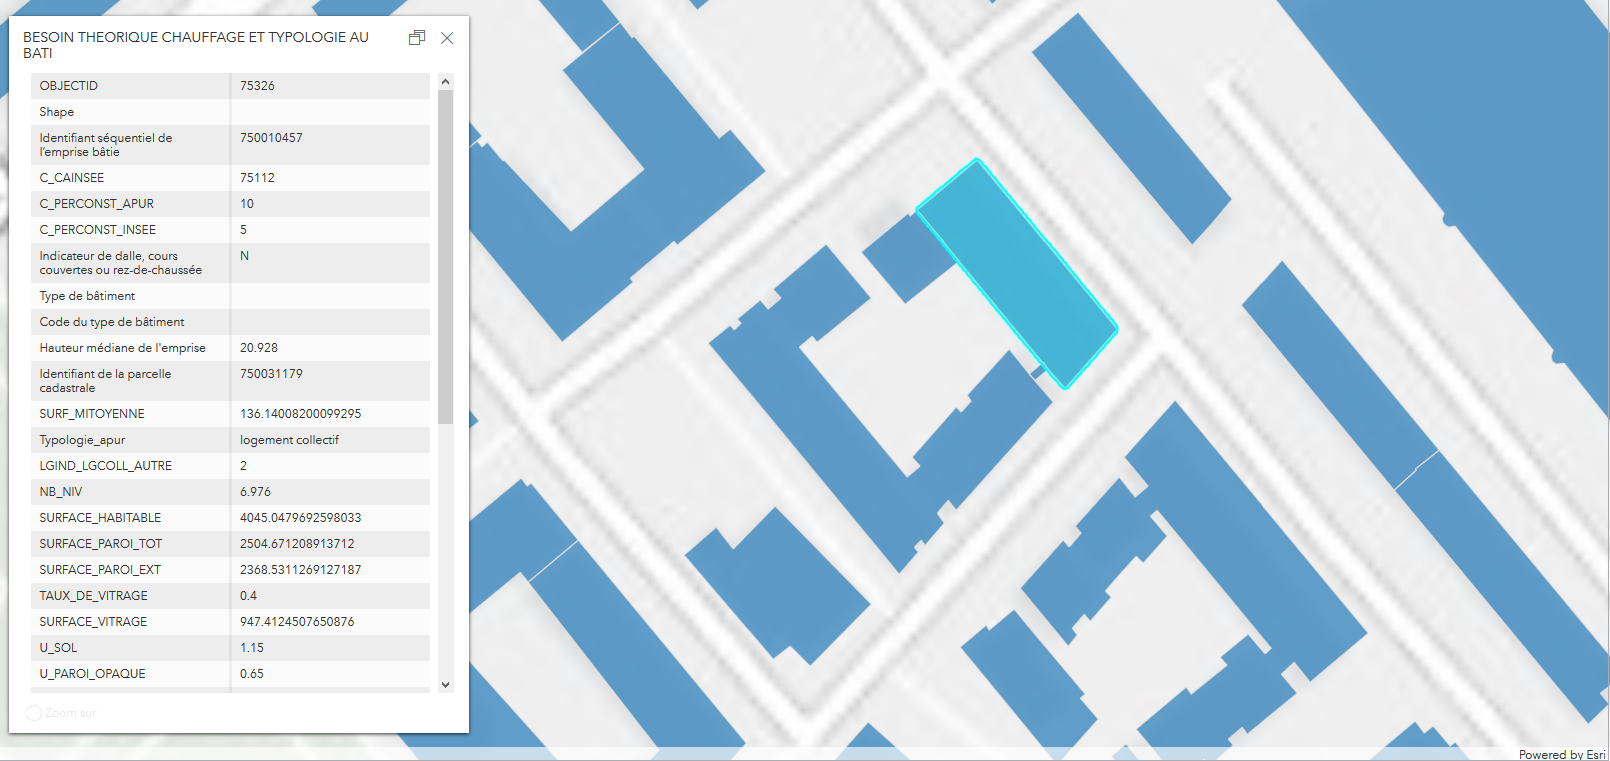
\includegraphics[width=0.9\linewidth]{__imgs/carte_apur} 

}

\caption[Prévisualisation des données sous forme de carte  -  \url{https://www.apur.org/open_data/}]{Prévisualisation des données sous forme de carte}\label{fig:carte_apur}
\end{figure}
\end{tcolorbox}

\begin{tcolorbox}
\begin{figure}

{\centering 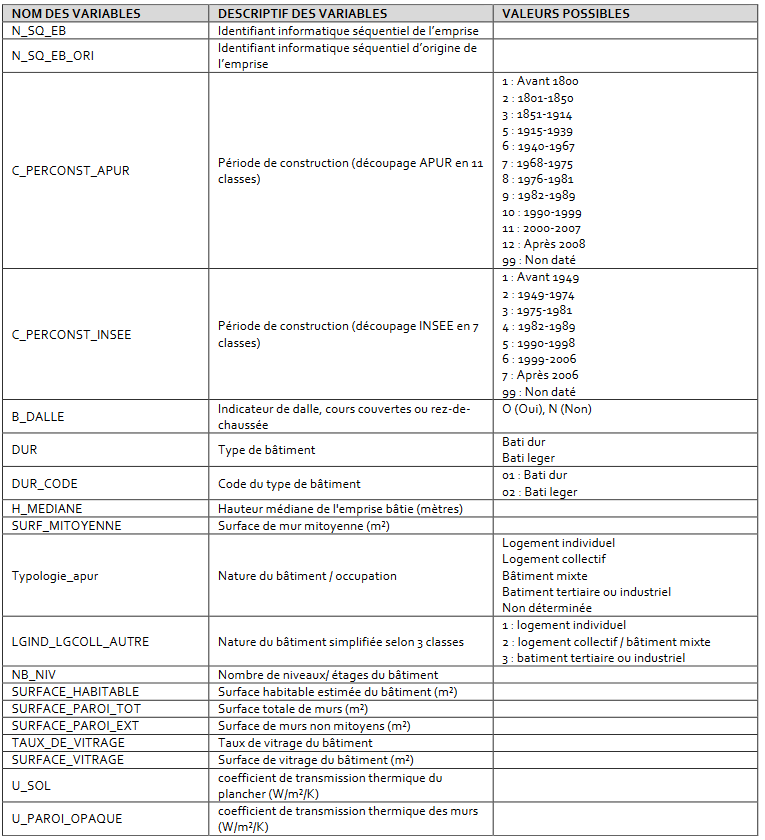
\includegraphics[width=0.9\linewidth]{__imgs/meta_apur} 

}

\caption[Des variables fournissant des informations précieuses sur l'existant  -  \url{https://www.apur.org/open_data/BESOIN_THEORIQUE_CHAUFFAGE_TYPO_BATI_OD.pdf}]{Des variables fournissant des informations précieuses sur l'existant}\label{fig:meta_apur}
\end{figure}
\end{tcolorbox}

Cependant, quelques opérations géométriques sont nécessaires à partir
des différentes variables afin d'extraire deux données quantitatives,
l'\textbf{épaisseur de la façade} ainsi que la \textbf{surface de
toiture}, pouvant être mises en oeuvre de manière triviale grâce à
Python au moment de l'extraction.

\begin{tcolorbox}
\begin{figure}

{\centering 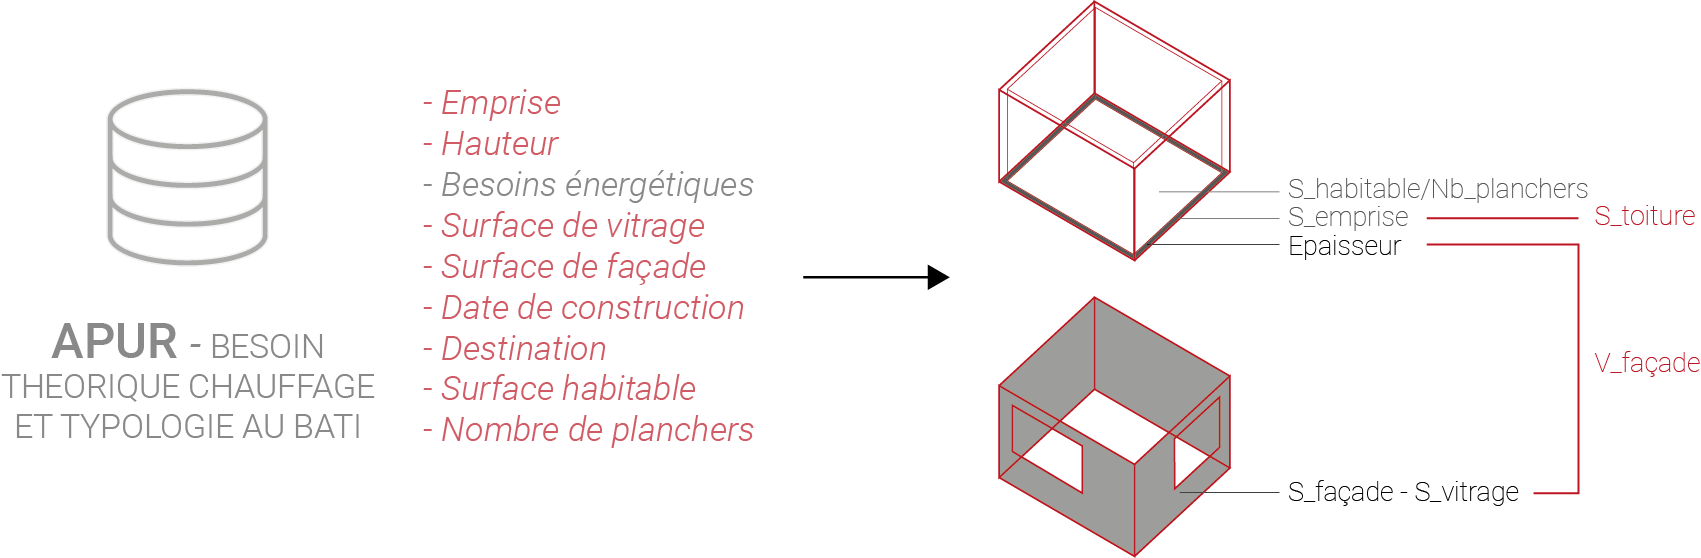
\includegraphics[width=0.9\linewidth]{__imgs/schema_apur} 

}

\caption[Opérations géométriques à effectuer à partir des données brutes  -  Réalisation personnelle]{Opérations géométriques à effectuer à partir des données brutes}\label{fig:schema_apur}
\end{figure}
\end{tcolorbox}

Ce jeu de données contenant également des informations sur la
\textbf{destination} ainsi que l'\textbf{époque de construction}, cela
pourrait également constituer deux variables à fournir en entrée de
l'algorithme, afin d'affiner la prédiction, puisqu'elles auront un lien
avec le type de matériau employé entre autres.\\
~\\
Dès lors, un second jeu de données doit être capable de fournir des
données concernant la \textbf{nature des matériaux} d'un bâtiment,
l'idéal étant qu'il provienne également de l'\emph{APUR} afin de
faciliter son recoupement via un identifiant propre à chaque bâtiment,
commun aux deux jeux de données. Or, un tel jeu n'existe actuellement
pas dans la base de l'\emph{APUR}.\\
~\\
Cependant, un autre jeu de données contenant des informations sur le
bâti existe sur une autre plateforme en Open Data mise en place par
l'\textbf{IGN}, intitulé la \textbf{BD TOPO}. Cette dernière est une
base de données vectorielle à l'échelle nationale constituée de
plusieurs \textbf{couches de données cartographiées et géolocalisées sur
de multiples domaines}, tels que les tracés des limites administratives,
les infrastructures de transports, l'hydrographie et plus
particulièrement \textbf{le bâti}. La plateforme d'IGN ne proposant pas
de moyens de prévisualisation, les métadonnées seront consultées dans un
premier temps.

\begin{tcolorbox}
\begin{figure}

{\centering 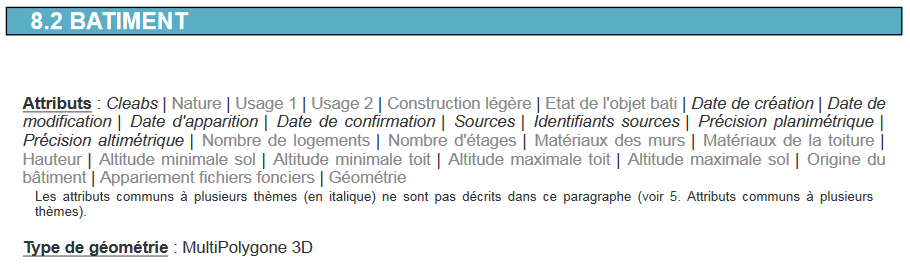
\includegraphics[width=0.9\linewidth]{__imgs/meta_ign} 

}

\caption[Extrait des métadonnées : attributs pour chaque bâtiment dans la BD TOPO  -  \url{https://qlf-geoservices.ign.fr/ressources_documentaires/Espace_documentaire/BASES_VECTORIELLES/BDTOPO/DC_BDTOPO_3-0.pdf}]{Extrait des métadonnées : attributs pour chaque bâtiment dans la BD TOPO}\label{fig:meta_ign}
\end{figure}
\end{tcolorbox}

Dès lors, ces données contiennent des attributs qui complètent à
merveille les données géométriques provenant de l'\emph{APUR}, à savoir
les \textbf{matériaux des murs} ainsi que les \textbf{matériaux de
toiture}.

\begin{tcolorbox}
\begin{figure}

{\centering 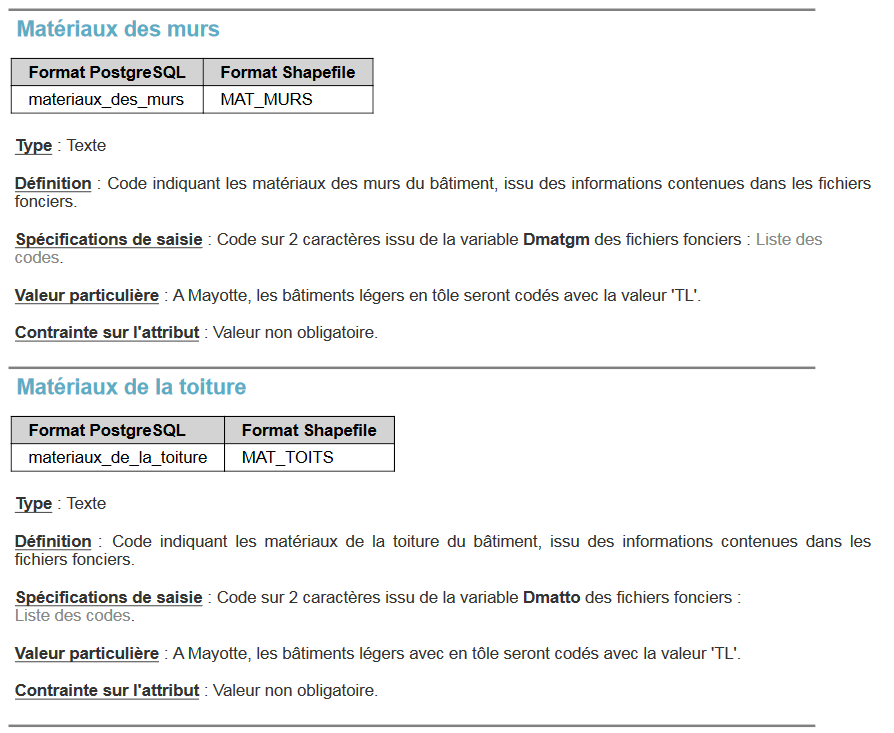
\includegraphics[width=0.9\linewidth]{__imgs/meta_ign_2} 

}

\caption[Extrait des métadonnées : détail des attributs concernant les matériaux  -  \url{https://qlf-geoservices.ign.fr/ressources_documentaires/Espace_documentaire/BASES_VECTORIELLES/BDTOPO/DC_BDTOPO_3-0.pdf}]{Extrait des métadonnées : détail des attributs concernant les matériaux}\label{fig:meta_ign_2}
\end{figure}
\end{tcolorbox}

\begin{tcolorbox}
\begin{figure}

{\centering 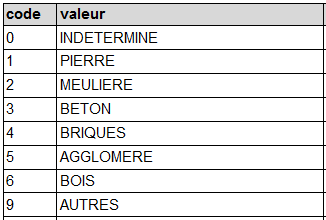
\includegraphics[height=0.3\textheight]{__imgs/matmur} 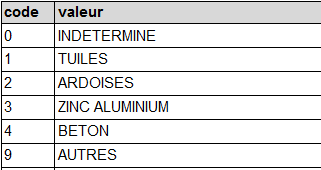
\includegraphics[height=0.3\textheight]{__imgs/mattoit} 

}

\caption[Extraits des tables des matériaux pour les murs (gauche) et les toitures (droite)  -  \url{http://piece-jointe-carto.developpement-durable.gouv.fr/NAT004/DTerNP/html3/annexes/}]{Extraits des tables des matériaux pour les murs (gauche) et les toitures (droite)}\label{fig:mats}
\end{figure}
\end{tcolorbox}

La plateforme d'IGN ne proposant pas de moyens de prévisualiser les
données sous la forme d'une carte, un petit script Python sera ici
utilisé afin de visualiser les données associées à un bâtiment grâce au
module \emph{GeoPandas} à partir du fichier des bâtiments au format
ShapeFile contenu dans la base de données une fois téléchargée.

\begin{tcolorbox}[title= Extraits des tables des matériaux pour les murs (gauche) et les toitures (droite) ,colback=boitecode]
\begin{lstlisting}[style=code]
import geopandas as gpd
data = gpd.read_file("F:\\BD_TOPO_IDF_\\BATI\\BATIMENT.shp")
print(data.head(1))\end{lstlisting}

```
ttvar{#}ttvar{#}                          ID          NATURE       USAGE1  USAGE2 LEGER        ETAT           DATE_CREAT             DATE_MAJ    DATE_APP DATE_CONF  ... MAT_MURS MAT_TOITS  HAUTEUR  Z_MIN_SOL  Z_MIN_TOIT  Z_MAX_TOIT Z_MAX_SOL ORIGIN_BAT  APP_FF                                           geometry
ttvar{#}ttvar{#} 0  BATIMENT0000000245492229  Indifférenciée  Résidentiel  Annexe   Non  En service  2010-11-25 12:44:09  2019-07-01 10:40:31  1920-01-01      None  ...       50        10      4.9       54.0        58.9        None      None   Cadastre   C 0.6  POLYGON Z ((663956.500 6869331.200 58.900, 663...
ttvar{#}ttvar{#} 
ttvar{#}ttvar{#} [1 rows x 26 columns]
```

\end{tcolorbox}

\begin{tcolorbox}
\begin{figure}

{\centering 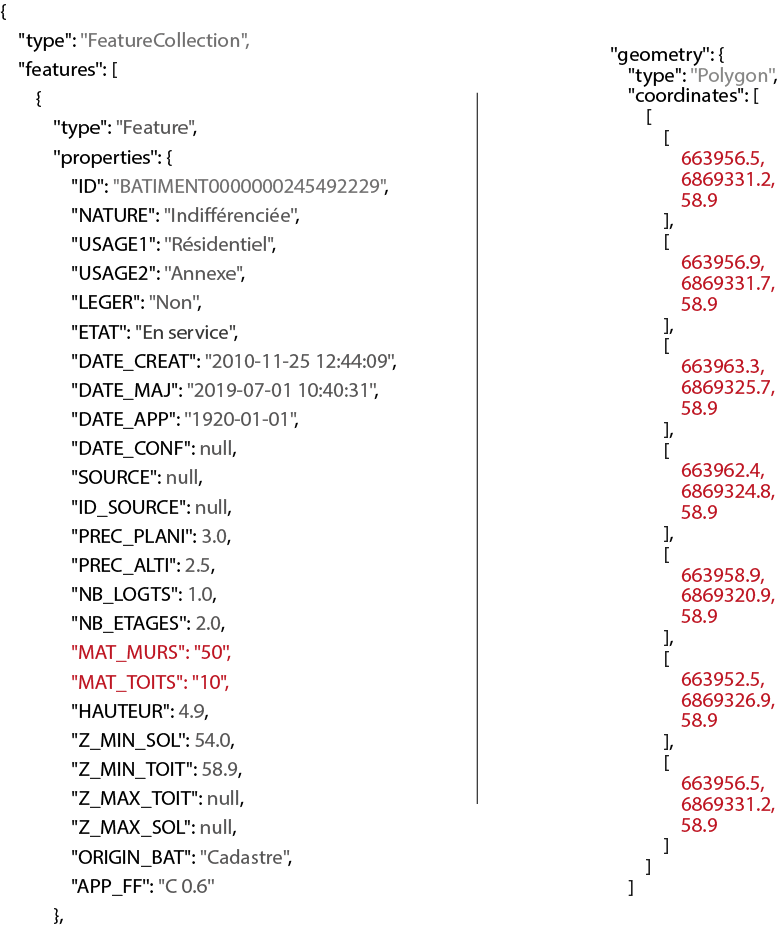
\includegraphics[width=0.9\linewidth]{__imgs/donnee_ign} 

}

\caption[Extraits des tables des matériaux pour les murs (gauche) et les toitures (droite)  -  \url{http://piece-jointe-carto.developpement-durable.gouv.fr/NAT004/DTerNP/html3/annexes/}]{Extraits des tables des matériaux pour les murs (gauche) et les toitures (droite)}\label{fig:donnee_ign}
\end{figure}
\end{tcolorbox}

Dès lors, le jeu actuel ne possédant aucun attribut à caractère
identifiant en commun avec le jeu de données de l'\emph{APUR}, les
\textbf{coordonnées terrestres} de l'emprise représentent \textbf{le
seul moyen} envisageable de les recouper, de sorte à ce que les
attributs concernant les matériaux dans la \emph{BD TOPO} soient ajoutés
au jeu de l'\emph{APUR}. En l'occurrence, les coordonnées ci-dessus sont
exprimées selon la notation \textbf{UTM}, que l'on peut aisément
manipuler grâce à Python comme l'ont montré les chapitres précédents.\\
~\\
Enfin, l'idéal serait de pouvoir fournir des \textbf{photographies} de
chaque bâtiment à l'algorithme, dans le but d'améliorer grandement sa
capacité à identifier les matériaux sur l'existant. Certains critères
doivent alors absolument être remplis :

\begin{itemize}
\item
  Ces images doivent être \textbf{disponibles pour une grande majorité
  des bâtiments} et être facilement \textbf{accessibles}
\item
  Les photographies doivent être prises du \textbf{même point de vue}
\item
  De préférence, chaque bâtiment sujet doit pouvoir être \textbf{isolé}
  (sur un fond blanc par exemple) afin d'améliorer sa détection.
\end{itemize}

\hfill\break
Il semble alors qu'actuellement, le type d'imagerie remplissant ces
trois critères soit l'\textbf{imagerie aérienne}. Ainsi, le jeu de
données \textbf{BD ORTHO HR} provenant du même organisme (IGN) sera ici
exploité. C'est une base de données constituée d'un quadrillage de
photographies aériennes en haute définition (de forme carrée de 25000
pixels de côté), dont chaque carreau représente 5 kilomètres de côté.
Chacun d'entre eux possède un fichier annexe où l'on retrouve les
\textbf{coordonnées terrestres aux 4 extrémités de l'image} (en
notations \emph{UTM}).\\
~\\
Ceci permettra ainsi d'isoler pour chaque bâtiment (dont on dipose des
coordonnées de l'emprise) une \textbf{photographie découpée} à partir de
ces photographies.

\begin{tcolorbox}
\begin{figure}

{\centering 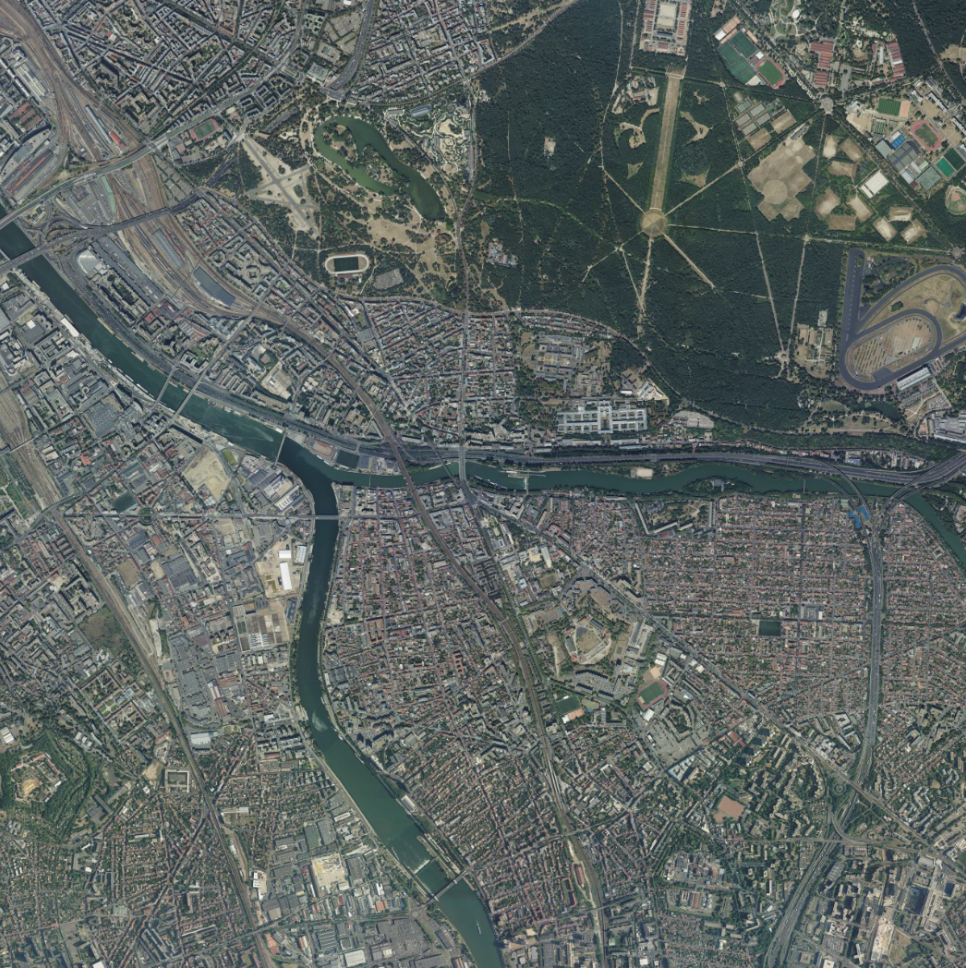
\includegraphics[width=0.45\linewidth]{__imgs/bd_ortho_img} 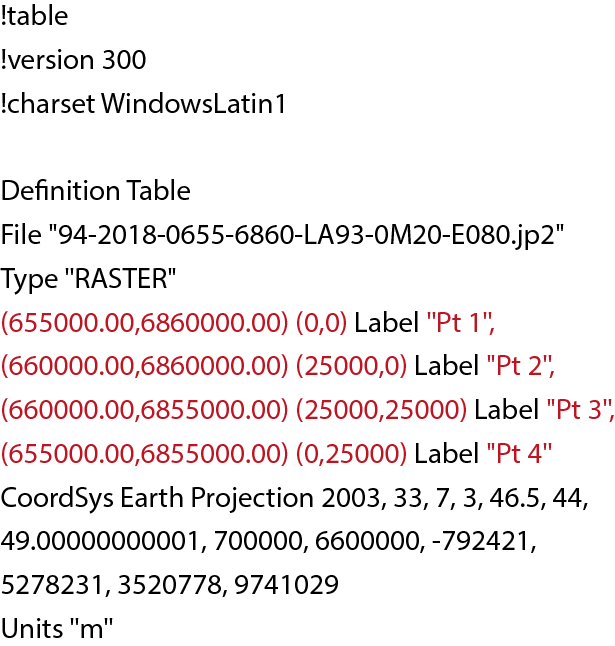
\includegraphics[width=0.45\linewidth]{__imgs/bd_ortho} 

}

\caption[Extrait d'un carreau de la BD ORTHO (gauche) et ses données de géolocalisation (droite)  -  \url{https://geoservices.ign.fr/}]{Extrait d'un carreau de la BD ORTHO (gauche) et ses données de géolocalisation (droite)}\label{fig:bd_ortho}
\end{figure}
\end{tcolorbox}

\hfill\break
\hfill\break
Ainsi, dans l'objectif de créer un jeu de données regroupant
suffisamment d'informations concernant les caractéristiques géométriques
des bâtiments existants et la nature de leurs principaux matériaux, il
s'avère nécessaire de \textbf{recouper plusieurs jeux de données}
produits par des \textbf{organismes différents} uniquement grâce à leur
\textbf{géolocalisation}. De plus, il existe une certaine hétérogénéité
des \textbf{types de données} à manipuler, puisque des \textbf{images}
viendront compléter des données \textbf{alphanumérique} (tel que les
dates ou les surfaces).\\
~\\
L'enjeu du langage Python est donc de permettre ce \textbf{recoupement
géométrique} entre les différents bâtiments.

\hypertarget{le-recoupement-guxe9omuxe9trique}{%
\subsubsection{Le recoupement
géométrique}\label{le-recoupement-guxe9omuxe9trique}}

\newpage

\hypertarget{ruxe9sultats-et-bilan-technique}{%
\subsection{Résultats et bilan
technique}\label{ruxe9sultats-et-bilan-technique}}

\hypertarget{entrauxeenement-du-moduxe8le}{%
\subsubsection{Entraînement du
modèle}\label{entrauxeenement-du-moduxe8le}}

\hypertarget{aperuxe7u-des-limites-actuelles}{%
\subsubsection{Aperçu des limites
actuelles}\label{aperuxe7u-des-limites-actuelles}}

\newpage

\hypertarget{conclusion}{%
\section*{CONCLUSION}\label{conclusion}}
\addcontentsline{toc}{section}{CONCLUSION}

Grâce à l'approche pratique proposée au sein de ce mémoire, nous avons
pu démontrer que le langage de programmation Python constitue un outil
souple et performant permettant de d'accompagner l'architecte tout au
long de son exploitation des données issues de l'Open Data.\\
~\\
En effet, permettant en premier lieu de rendre compréhensible et
manipulable aux plus novices les structures de données couramment
rencontrées, en particulier les données hiérarchisées hétérogènes, le
langage est doté d'outils de production de documents synthétiques tout à
fait capables de convertir les données extraites en formats de fichiers
courants pour l'architecte, élément primordial au sein du « workflow »
de l'architecte. Ainsi, au-delà des graphiques statistiques, Python
permet la génération de cartographies interactives, mais surtout des
dessins techniques hiérarchisés et même des modèles 3D de manière
automatique et personnalisée, représentant un gain de temps
considérable.\\
~\\
Enfin, l'architecte devient capable grâce à Python de mener ses propres
analyses de données afin de les mettre à profit dans son activité de
conception, grâce à une capacité d'identification de corrélations entre
différentes données agrégées, ou encore celle de pouvoir prédire
l'impact de son intervention grâce au Machine Learning.\\
~\\
De plus, épaulé par divers modules permettant tous ces usages de manière
simplifiée tout au long du processus d'exploitation des données
ouvertes, le Python acquiert un véritable caractère universel, autant
dans le sens où il est capable de se suffire à lui-même que pour
qualifier sa compatibilité extraordinaire avec d'autres outils et
services (comme Rhinoceros).\\
~\\
Au-delà du cadre de l'exploitation des données issues de l'Open Data, ce
langage représente un véritable pivot afin d'accompagner les agences
vers les nouveaux outils plus intelligents.\\
~\\
Premièrement, l'expérience acquise durant la manipulation des jeux de
données ouverts (en particulier sur les notions des structures de
données) sera extrêmement précieuse lorsqu'il s'agira d'exploiter des
jeux de données plus directement liés à la pratique architecturale en
elle-même, comme depuis un parc de « Smart Buildings » qu'il faudra
surveiller et analyser par exemple.\\
~\\
Au-delà de cet aspect, des solutions logicielles émergentes tel que «
Générative Design in Revit » publiée par Autodesk,\footnote{\emph{Generative
  Design in Revit now available. Revit} {[}en~ligne{]}. 8 avril 2020.
  {[}Consulté~le~17~janvier~2021{]}. Disponible à l'adresse\,:
  \url{https://blogs.autodesk.com/revit/2020/04/08/generative-design-in-revit/}.
  Section: What's New.} désormais intégrée à Revit 2021 proposent déjà à
l'architecte de travailler aux côtés d'algorithmes évolutifs et
prédictifs, que ce soit de manière simplifiée par interface graphique ou
bien personnalisable grâce au langage de programmation visuelle Dynamo.
La collaboration entre des agences d'architecture et des solutions
intégrant de l'Intelligence Artificielle commence également à se
développer, tel que l'agence \emph{Valode\&Pistre} et son partenariat
avec « SpaceMaker AI»,\footnote{\emph{Valode\&Pistre se lance dans
  l'aventure de l'IA} {[}en~ligne{]}. 8 février 2021. Disponible à
  l'adresse\,:
  \url{https://www.cahiers-techniques-batiment.fr/article/valode-pistre-se-lance-dans-l-aventure-de-l-ia.45391}.}
société norvégienne spécialisée dans la conception urbaine générative.\\
~\\
Ainsi, de nouvelles solutions sont développées chaque année, mais il
existera toujours un besoin de \textbf{programmer des outils} pour
différents types de projet et d'applications au sein de ces derniers,
telle que l'insertion urbaine, la conception de l'enveloppe ou encore la
question des usages.

\hfill\break
\hfill\break
Toutes ces opportunités nouvelles requièrent une certaine familiarité
avec le fonctionnement algorithmique, et surtout une assimilation de sa
manière de fonctionner afin de l'intégrer efficacement à son « workflow
»\\
~\\
Dès lors, de par son statut de langage de programmation lui conférant un
caractère universel quant aux notions de bases informatiques et surtout
algorithmiques (même avec une syntaxe simplifiée), le Python se présente
comme un atout « futur-proof » face à ces nouvelles interactions
architecte-machine. De plus, l'adoption massive du Python par les
architectes permettrait d'amorcer une solution efficace afin de lutter
contre la crainte de la montée en puissance de l'Intelligence
Artificielle au sein des métiers du bâtiment, par une atténuation
considérable de l'effet « Boite noire » qu'elle suscite. Ceci
faciliterait donc grandement la transition du corps architectural dans
la numérisation du domaine du bâtiment.\\
~\\
Au-delà de cette appropriation, une certaine motivation de créer des
outils logiciels par les architectes pour les architectes intégrant ces
nouvelles compétences pourrait émerger, permettant alors de réaffirmer
la place du métier d'architecte au sein d'un écosystème de plus en plus
techno-centré.

\newpage

\hypertarget{bibliographie}{%
\section*{BIBLIOGRAPHIE}\label{bibliographie}}
\addcontentsline{toc}{section}{BIBLIOGRAPHIE}

\hypertarget{refs}{}
\begin{CSLReferences}{0}{0}
\leavevmode\hypertarget{ref-opendataapur}{}%
\emph{Atelier Parisien d'Urbanisme} {[}en~ligne{]}. {[}s.~d.{]}.
{[}Consulté~le~4~février~2021{]}. Disponible à l'adresse\,:
\url{https://opendata.apur.org/}

\leavevmode\hypertarget{ref-arcgis2}{}%
\emph{Automate Road Surface Investigation Using Deep Learning \textbar{}
ArcGIS for Developers} {[}en~ligne{]}. {[}s.~d.{]}.
{[}Consulté~le~3~février~2021{]}. Disponible à l'adresse\,:
\url{https://developers.arcgis.com/python/sample-notebooks/automate-road-surface-investigation-using-deep-learning/}

\leavevmode\hypertarget{ref-mdsynt}{}%
\emph{Daring Fireball: Markdown Syntax Documentation} {[}en~ligne{]}.
{[}s.~d.{]}. {[}Consulté~le~5~février~2021{]}. Disponible à l'adresse\,:
\url{https://daringfireball.net/projects/markdown/syntax}

\leavevmode\hypertarget{ref-etalab}{}%
\emph{Etalab - Qui sommes-nous. Le blog d'Etalab} {[}en~ligne{]}.
{[}s.~d.{]}. {[}Consulté~le~17~janvier~2021{]}. Disponible à
l'adresse\,: \url{https://www.etalab.gouv.fr/qui-sommes-nous}

\leavevmode\hypertarget{ref-gdrevit}{}%
\emph{Generative Design in Revit now available. Revit} {[}en~ligne{]}. 8
avril 2020. {[}Consulté~le~17~janvier~2021{]}. Disponible à l'adresse\,:
\url{https://blogs.autodesk.com/revit/2020/04/08/generative-design-in-revit/}.
Section: What's New

\leavevmode\hypertarget{ref-ign}{}%
\emph{Géoservices \textbar{} Accéder au téléchargement des données
libres IGN} {[}en~ligne{]}. {[}s.~d.{]}.
{[}Consulté~le~15~septembre~2020{]}. Disponible à l'adresse\,:
\url{https://geoservices.ign.fr/documentation/diffusion/telechargement-donnees-libres.html}

\leavevmode\hypertarget{ref-ouvdonpub}{}%
\emph{L'ouverture des données publiques. Gouvernement.fr}
{[}en~ligne{]}. {[}s.~d.{]}. {[}Consulté~le~17~janvier~2021{]}.
Disponible à l'adresse\,:
\url{https://www.gouvernement.fr/action/l-ouverture-des-donnees-publiques}

\leavevmode\hypertarget{ref-matplotlib}{}%
\emph{Matplotlib : Python plotting} {[}en~ligne{]}. {[}s.~d.{]}.
{[}Consulté~le~16~janvier~2021{]}. Disponible à l'adresse\,:
\url{https://matplotlib.org/}

\leavevmode\hypertarget{ref-metacity}{}%
\emph{MVRDV - Metacity / Datatown} {[}en~ligne{]}. 8 février 2021.
Disponible à l'adresse\,:
\url{https://www.mvrdv.nl/projects/147/metacity-\%2F-datatown-}

\leavevmode\hypertarget{ref-mvrdv}{}%
\emph{MVRDV - NEXT} {[}en~ligne{]}. 8 février 2021. Disponible à
l'adresse\,: \url{https://www.mvrdv.nl/themes/15/next}

\leavevmode\hypertarget{ref-ademe}{}%
\emph{Portail open data de l'ADEME} {[}en~ligne{]}. {[}s.~d.{]}.
{[}Consulté~le~17~janvier~2021{]}. Disponible à l'adresse\,:
\url{https://data.ademe.fr/}

\leavevmode\hypertarget{ref-idfmobi}{}%
\emph{Portail Open data Île-de-France Mobilités} {[}en~ligne{]}.
{[}s.~d.{]}. {[}Consulté~le~17~janvier~2021{]}. Disponible à
l'adresse\,: \url{https://data.iledefrance-mobilites.fr/pages/home/}

\leavevmode\hypertarget{ref-pyopengl}{}%
\emph{PyOpenGL -- The Python OpenGL Binding} {[}en~ligne{]}. 24 janvier
2021. Disponible à l'adresse\,: \url{http://pyopengl.sourceforge.net/}

\leavevmode\hypertarget{ref-pytorch}{}%
\emph{PyTorch} {[}en~ligne{]}. {[}s.~d.{]}.
{[}Consulté~le~20~janvier~2021{]}. Disponible à l'adresse\,:
\url{https://pytorch.org/}

\leavevmode\hypertarget{ref-oracle}{}%
\emph{Qu'est-ce qu'une base de données publiques ? \textbar{} Oracle
France} {[}en~ligne{]}. 8 février 2021. Disponible à l'adresse\,:
\url{https://www.oracle.com/fr/database/base-donnees-publique-definition.html}

\leavevmode\hypertarget{ref-rhinoinside}{}%
\emph{Rhino - Rhino.Inside} {[}en~ligne{]}. 25 janvier 2021. Disponible
à l'adresse\,: \url{https://www.rhino3d.com/features/rhino-inside/}

\leavevmode\hypertarget{ref-sklearn}{}%
\emph{scikit-learn: machine learning in Python} {[}en~ligne{]}.
{[}s.~d.{]}. {[}Consulté~le~16~janvier~2021{]}. Disponible à
l'adresse\,: \url{https://scikit-learn.org/stable/}

\leavevmode\hypertarget{ref-seaborn}{}%
\emph{Seaborn : statistical data visualization} {[}en~ligne{]}.
{[}s.~d.{]}. {[}Consulté~le~28~janvier~2021{]}. Disponible à
l'adresse\,: \url{https://seaborn.pydata.org/}

\leavevmode\hypertarget{ref-arcgis1}{}%
\emph{Spatial and temporal distribution of service calls using big data
tools \textbar{} ArcGIS for Developers} {[}en~ligne{]}. {[}s.~d.{]}.
{[}Consulté~le~3~février~2021{]}. Disponible à l'adresse\,:
\url{https://developers.arcgis.com/python/sample-notebooks/spatial-and-temporal-trends-of-service-calls/}

\leavevmode\hypertarget{ref-tensorflow}{}%
\emph{TensorFlow} {[}en~ligne{]}. {[}s.~d.{]}.
{[}Consulté~le~20~janvier~2021{]}. Disponible à l'adresse\,:
\url{https://www.tensorflow.org/}

\leavevmode\hypertarget{ref-pythondataviz}{}%
\emph{The Python Graph Gallery : Visualizing data with Python}
{[}en~ligne{]}. {[}s.~d.{]}. {[}Consulté~le~28~janvier~2021{]}.
Disponible à l'adresse\,: \url{https://python-graph-gallery.com/}

\leavevmode\hypertarget{ref-uberopen}{}%
\emph{Uber Movement: Let's find smarter ways forward, together.}
{[}en~ligne{]}. 8 février 2021. Disponible à l'adresse\,:
\url{https://movement.uber.com/cities?lang=fr-FR}

\leavevmode\hypertarget{ref-valodepistre}{}%
\emph{Valode\&Pistre se lance dans l'aventure de l'IA} {[}en~ligne{]}. 8
février 2021. Disponible à l'adresse\,:
\url{https://www.cahiers-techniques-batiment.fr/article/valode-pistre-se-lance-dans-l-aventure-de-l-ia.45391}

\leavevmode\hypertarget{ref-opendataeu}{}%
\emph{What is open data?} {[}en~ligne{]}. {[}s.~d.{]}.
{[}Consulté~le~28~décembre~2020{]}. Disponible à l'adresse\,:
\url{https://www.europeandataportal.eu/elearning/en/module1/\#/id/co-01}

\leavevmode\hypertarget{ref-hugel_cityengine-twitter_2014}{}%
HÜGEL, Stephan et ROUMPANI, Flora. \emph{{CityEngine}-Twitter}
{[}logiciel{]}. {[}S.~l.{]}\,: Zenodo, 14 mai 2014.
{[}Consulté~le~28~décembre~2020{]}.
DOI~\href{https://doi.org/10.5281/ZENODO.9795}{10.5281/ZENODO.9795}

\leavevmode\hypertarget{ref-pyopenglcrit}{}%
P.ROUGIER, Nicolas. \emph{Python \& OpenGL for Scientific
Visualization}. Bordeaux\,: {[}s.~n.{]}, 2018. Disponible à l'adresse\,:
\url{https://www.labri.fr/perso/nrougier/python-opengl/}

\leavevmode\hypertarget{ref-iavulga}{}%
VANNIEUWENHUYZE, Aurélien. \emph{Intelligence artificielle vulgarisée:
le Machine Learning et le Deep Learning par la pratique}. {[}S.~l.{]}\,:
{[}s.~n.{]}, 2019.
ISBN~\href{https://worldcat.org/isbn/978-2-409-02073-5}{978-2-409-02073-5}.
{OCLC}: 1127535504

\leavevmode\hypertarget{ref-Zhou2018}{}%
ZHOU, Qian-Yi, PARK, Jaesik et KOLTUN, Vladlen. {Open3D}: {A} Modern
Library for {3D} Data Processing. \emph{arXiv:1801.09847}. 2018

\end{CSLReferences}

\newpage

\hypertarget{iconographie}{%
\section*{ICONOGRAPHIE}\label{iconographie}}
\addcontentsline{toc}{section}{ICONOGRAPHIE}

\renewcommand{\listfigurename}{}

\listoffigures

\newpage

\hypertarget{annexe-un-muxe9moire-ruxe9diguxe9-en-r-markdown}{%
\section*{ANNEXE : UN MÉMOIRE RÉDIGÉ EN R
MARKDOWN}\label{annexe-un-muxe9moire-ruxe9diguxe9-en-r-markdown}}
\addcontentsline{toc}{section}{ANNEXE : UN MÉMOIRE RÉDIGÉ EN R MARKDOWN}

\linespread{2.0}

Ce mémoire a été rédigé dans son intégralité en utilisant le langage
\textbf{R markdown}, sous la forme d'un seul script.\\
~\\
Ce langage est basé en grande partie sur la syntaxe
\textbf{Markdown},\footnote{\emph{Daring Fireball: Markdown Syntax
  Documentation} {[}en~ligne{]}. {[}s.~d.{]}.
  {[}Consulté~le~5~février~2021{]}. Disponible à l'adresse\,:
  \url{https://daringfireball.net/projects/markdown/syntax}.} dont le
but est de prodiguer un moyen de rédiger des documents textuels de
manière \textbf{simplifiée} et \textbf{souple}, exportable dans une
multitude de supports, du format HTML (pour un affichage web) au format
PDF paginé pour impression.

\begin{tcolorbox}
\begin{figure}

{\centering 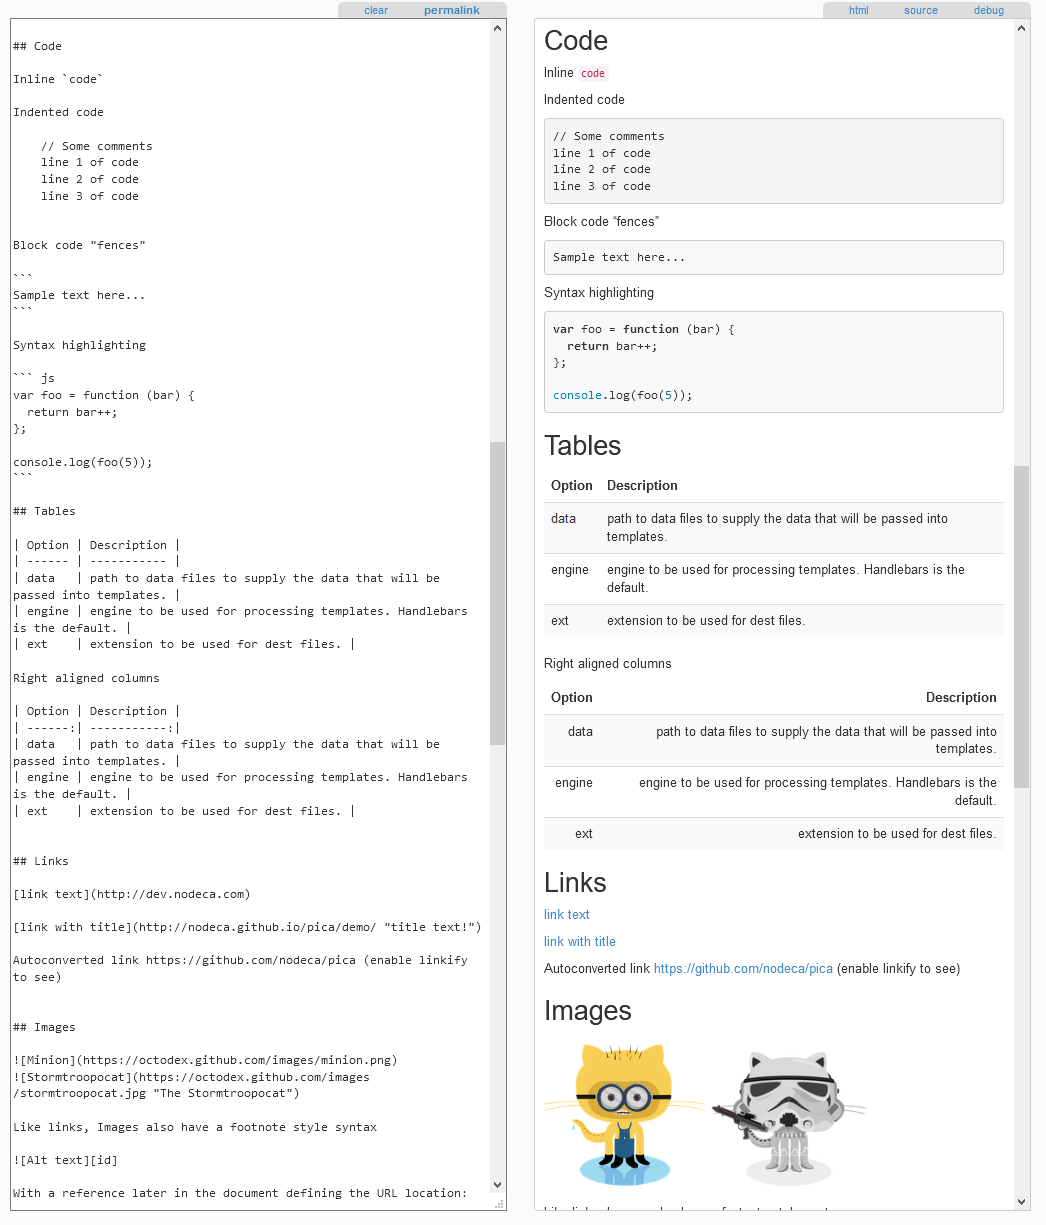
\includegraphics[width=0.9\linewidth]{__imgs/markdown} 

}

\caption[Un langage à la fois complet et souple à la syntaxe composée exclusivement de caractères spéciaux  -  https://markdown-it.github.io/]{Un langage à la fois complet et souple à la syntaxe composée exclusivement de caractères spéciaux}\label{fig:markdown}
\end{figure}
\end{tcolorbox}

Dans le cadre du mémoire, je me suis plutôt orienté sur son dérivé
augmenté par le langage de programmation \textbf{R} (d'où le nom de
\emph{R markdown}) pour les raisons suivantes :

\begin{itemize}
\item
  Là où le \emph{Markdown} permet uniquement d'afficher du code, il est
  possible ici \textbf{d'éxecuter du code directement au sein du
  document.} Le tout reste hautement configurable, permettant
  l'affichage des données en sortie (output), ainsi que de gérer la mise
  en forme graphique.
\item
  Grâce à un autre logiciel nommé \textbf{LaTeX}, il est possible d'y
  intégrer facilement des \textbf{références bibliographiques}, via un
  fichier .bib contenant les différents ouvrages et leurs informations,
  en pouvant spécifier la norme des références. La gestion des
  \textbf{images et figurés} est également facilitée, avec une
  numérotation ainsi qu'une iconographie générée automatiquement tout en
  restant paramétrable.
\item
  L'insertion de caractères relatifs \textbf{aux notations
  mathématiques} est également facilitée, pouvant s'avérer extrêmement
  utile.
\item
  Il sera possible \textbf{avec peu de changements} à apporter au script
  d'exporter facilement mon mémoire vers d'autres formats
  (HTML/DOCX/etc..) à l'avenir.
\end{itemize}

Cependant, bien que cette solution se soit révélée d'une praticité
redoutable dans le cadre de mon mémoire, il me paraît important de
souligner les quelques difficultés rencontrées.

\begin{itemize}
\tightlist
\item
  Là où le \emph{Markdown} ne requiert le plus souvent aucune
  installation tierce pour fonctionner (étant la plupart du temps
  intégré directement aux éditeurs de texte), la liste de programmes à
  installer est ici assez conséquente. En plus du langage \textbf{R}, ce
  sont au total \textbf{trois solutions logicielles} qui sont réclamées
  afin de pouvoir générer un fichier PDF (avec LaTeX pesant notamment
  entre 7 et 8Go).
\end{itemize}

\begin{tcolorbox}
\begin{figure}

{\centering 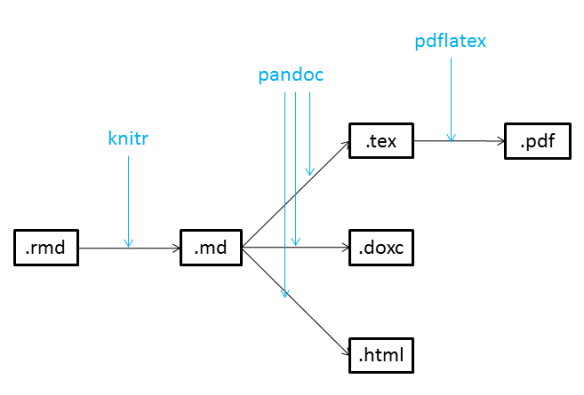
\includegraphics[width=0.9\linewidth]{__imgs/pandoc1} 

}

\caption[Outils et formats intermédiaires utilisés pour générer un fichier PDF  -  https://markdown-it.github.io/]{Outils et formats intermédiaires utilisés pour générer un fichier PDF}\label{fig:pandoc}
\end{figure}
\end{tcolorbox}

\begin{itemize}
\item
  L'utilisation de \textbf{LaTeX}, \textbf{Pandocs} et \textbf{Knitr} en
  plus du \emph{R markdown} permet une large palette de paramétrage, que
  l'on paye parfois au prix \textbf{d'incompatibilités entre certaines
  options présentes sur plusieurs de ces programmes à la fois}.
\item
  Enfin, le point le plus frustrant a été \textbf{le manque de
  documentation officielle sur certaines fonctionnalités}. Bien que l'on
  puisse y pallier grâce aux forums entre autres, cela représente
  l'antithèse de la simplicité du \emph{Markdown}, dont la documentation
  de qualité foisonne sur internet.
\end{itemize}

Malgré ces défauts, cela reste un moyen efficace de rédiger un document
de recherche tel qu'un mémoire, et encore davantage pour des documents
plus conséquents comme une thèse. Cependant, je souhaiterais explorer
d'autres outils similaires moins répandus mais plus minimalistes dans
leur approche comme le \textbf{Groff}, afin de déterminer quelle
solution est à la fois complète, simple et souple.

\end{document}
